\documentclass{article}
\usepackage{amsmath}
\usepackage{pdfpages}
\usepackage{float}
\usepackage{multicol}
\usepackage{multirow}
\usepackage{graphicx}
\usepackage[portrait, paperwidth=15cm, paperheight=30cm, left=0mm, top=0mm, bottom=0mm, right=0mm, margin=0mm]{geometry}
\graphicspath {{figures/}}
\usepackage{subfig}
% package for including graphics with figure-environment
\usepackage{hyperref}
% colored borders (false) colored text (true)
\hypersetup{colorlinks=true,citecolor=blue,filecolor=black,linkcolor=blue,urlcolor=blue}
%\textwidth=20cm
\begin{document}
\section{Fake closure tests}

\begin{figure}[!h]
\centering
  \subfloat[$m_{jj}$]{
      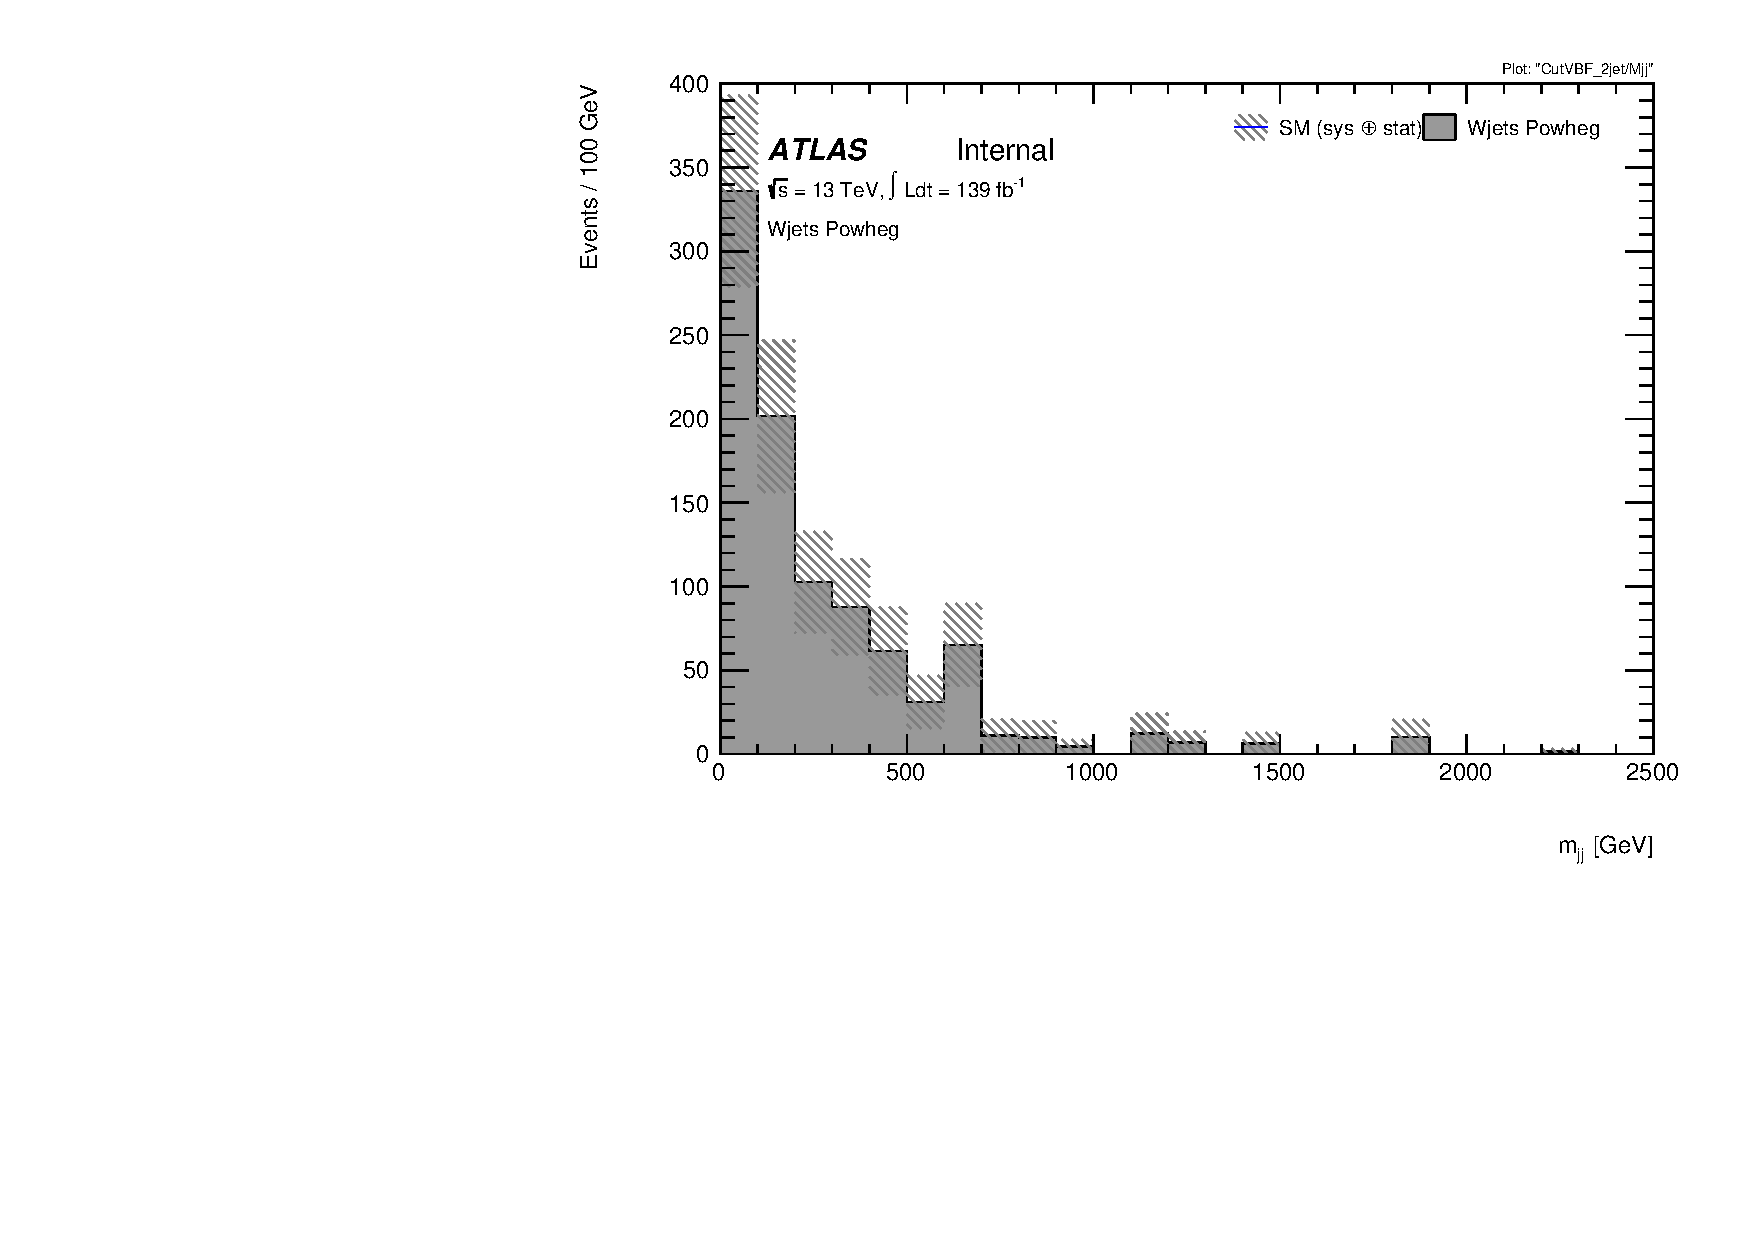
\includegraphics[width=0.3\textwidth]{FakeClosure/run2-emme-CutVBF_2jet-Mjj-lin.pdf}
  }\hfill
  \subfloat[$p^H_{T}$]{
      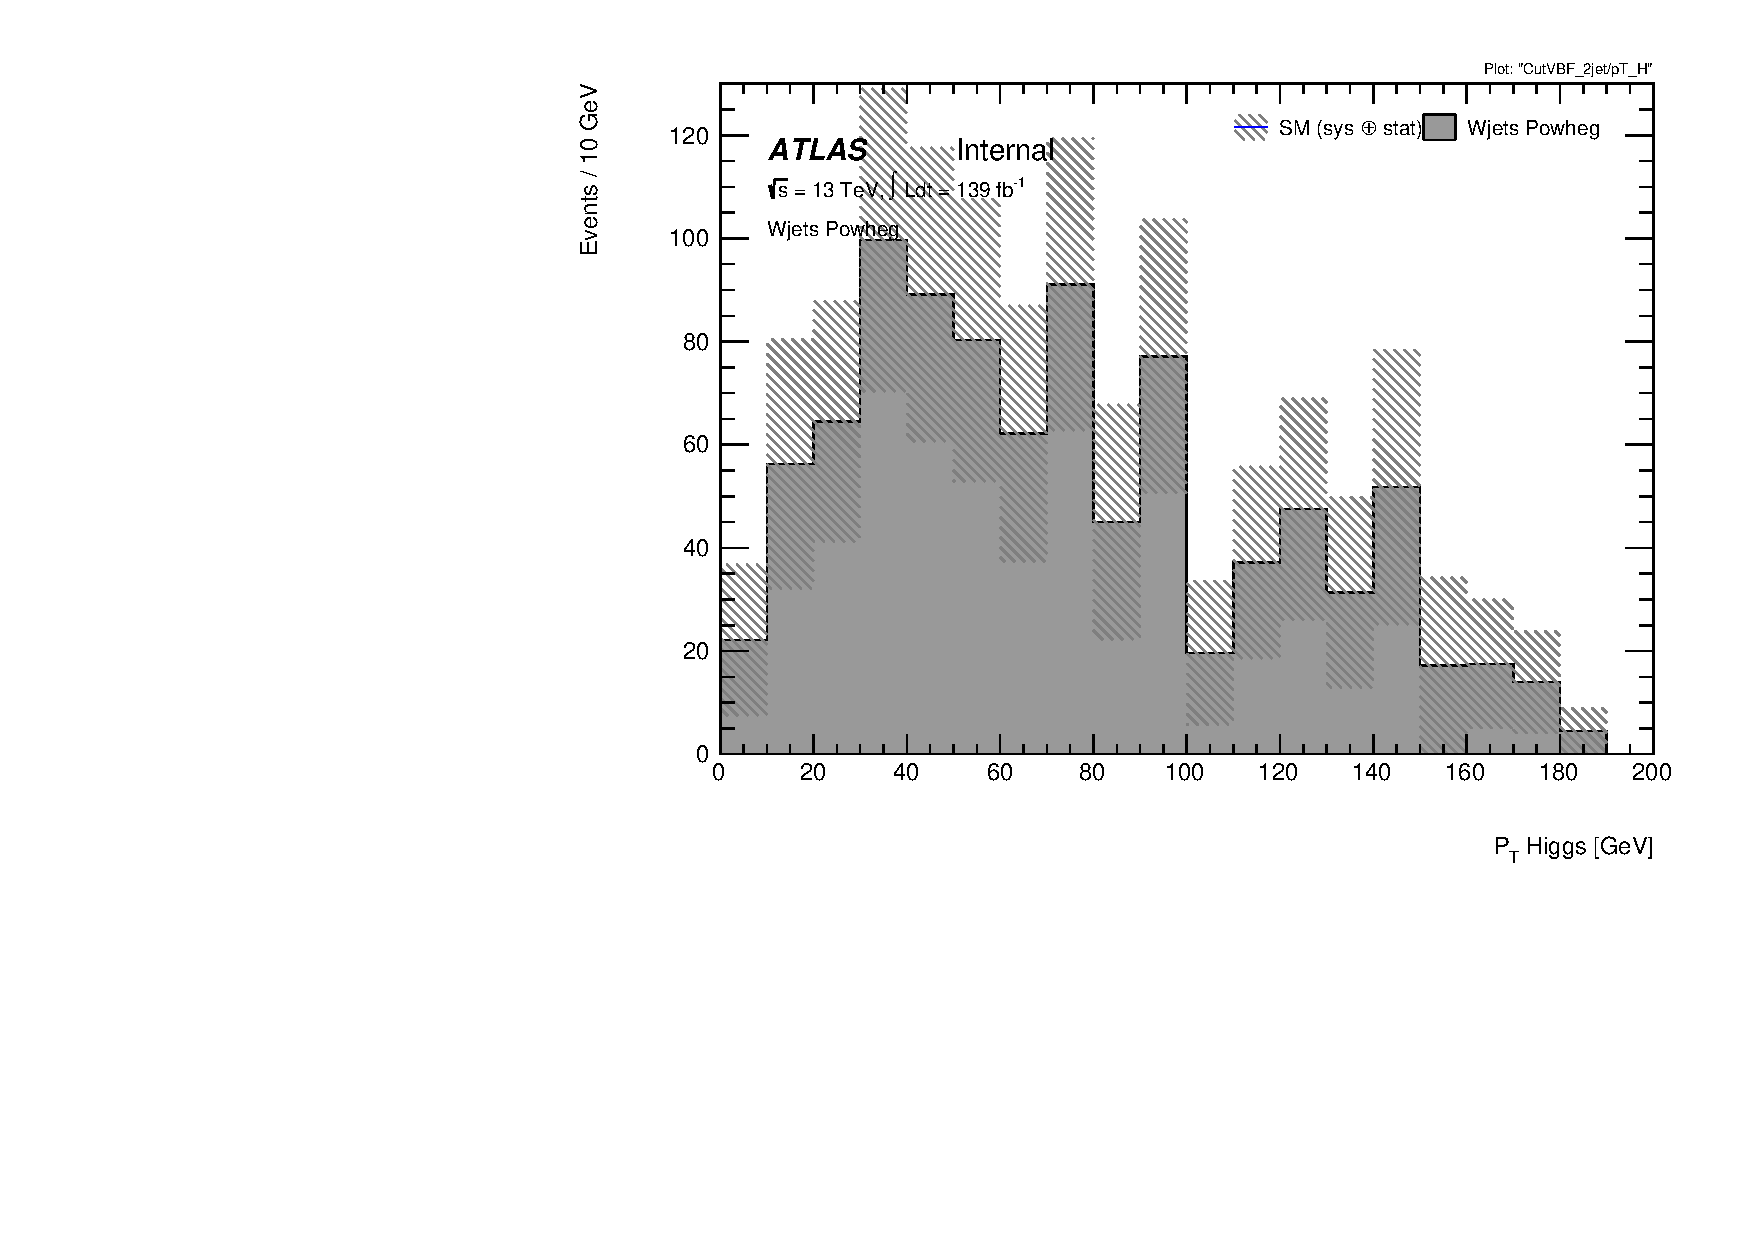
\includegraphics[width=0.3\textwidth]{FakeClosure/run2-emme-CutVBF_2jet-pT_H-lin.pdf}
  }\hfill
  \subfloat[$p_T^{l0}$]{
      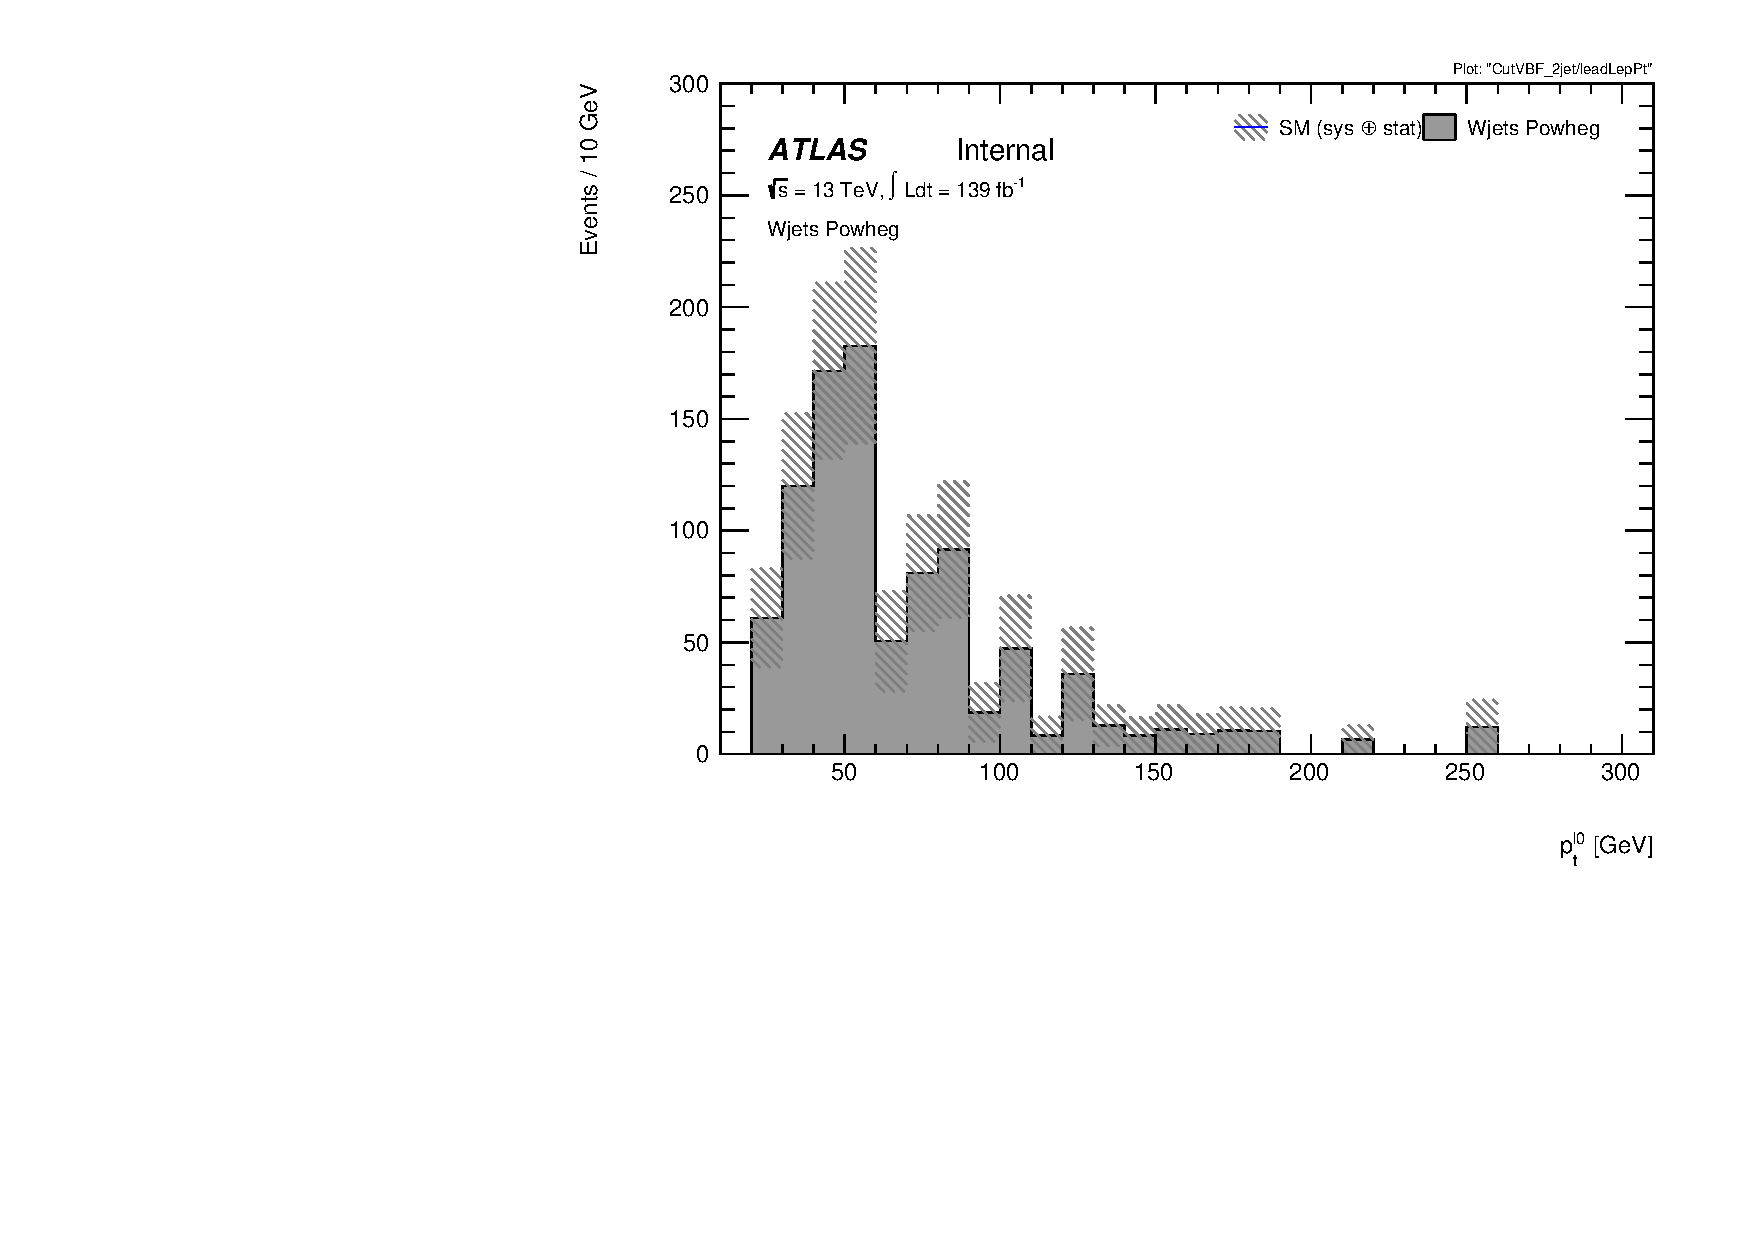
\includegraphics[width=0.3\textwidth]{FakeClosure/run2-emme-CutVBF_2jet-leadLepPt-lin.pdf}
  }\hfill
  \subfloat[$p_T^{l1}$]{
      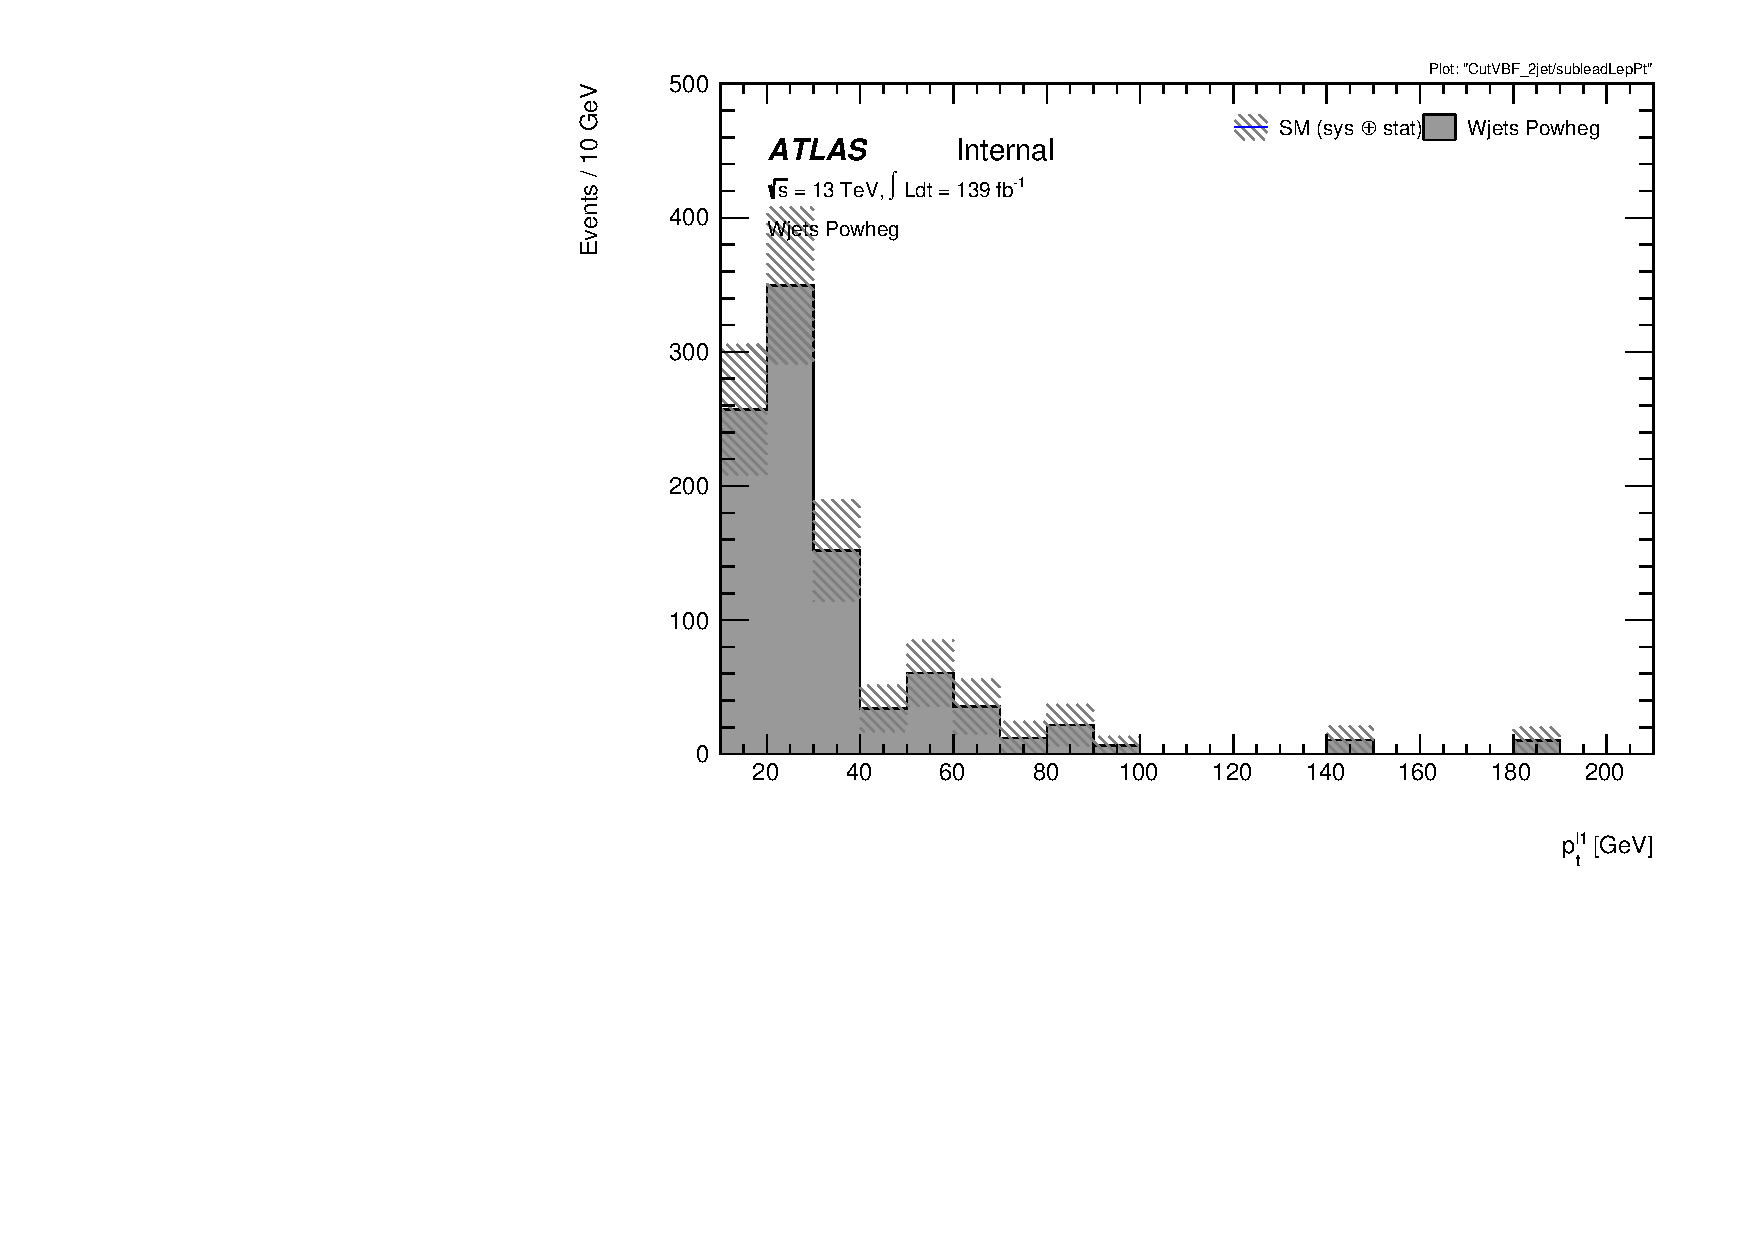
\includegraphics[width=0.3\textwidth]{FakeClosure/run2-emme-CutVBF_2jet-subleadLepPt-lin.pdf}
  }\hfill
  \subfloat[$p_T^{j0}$]{
      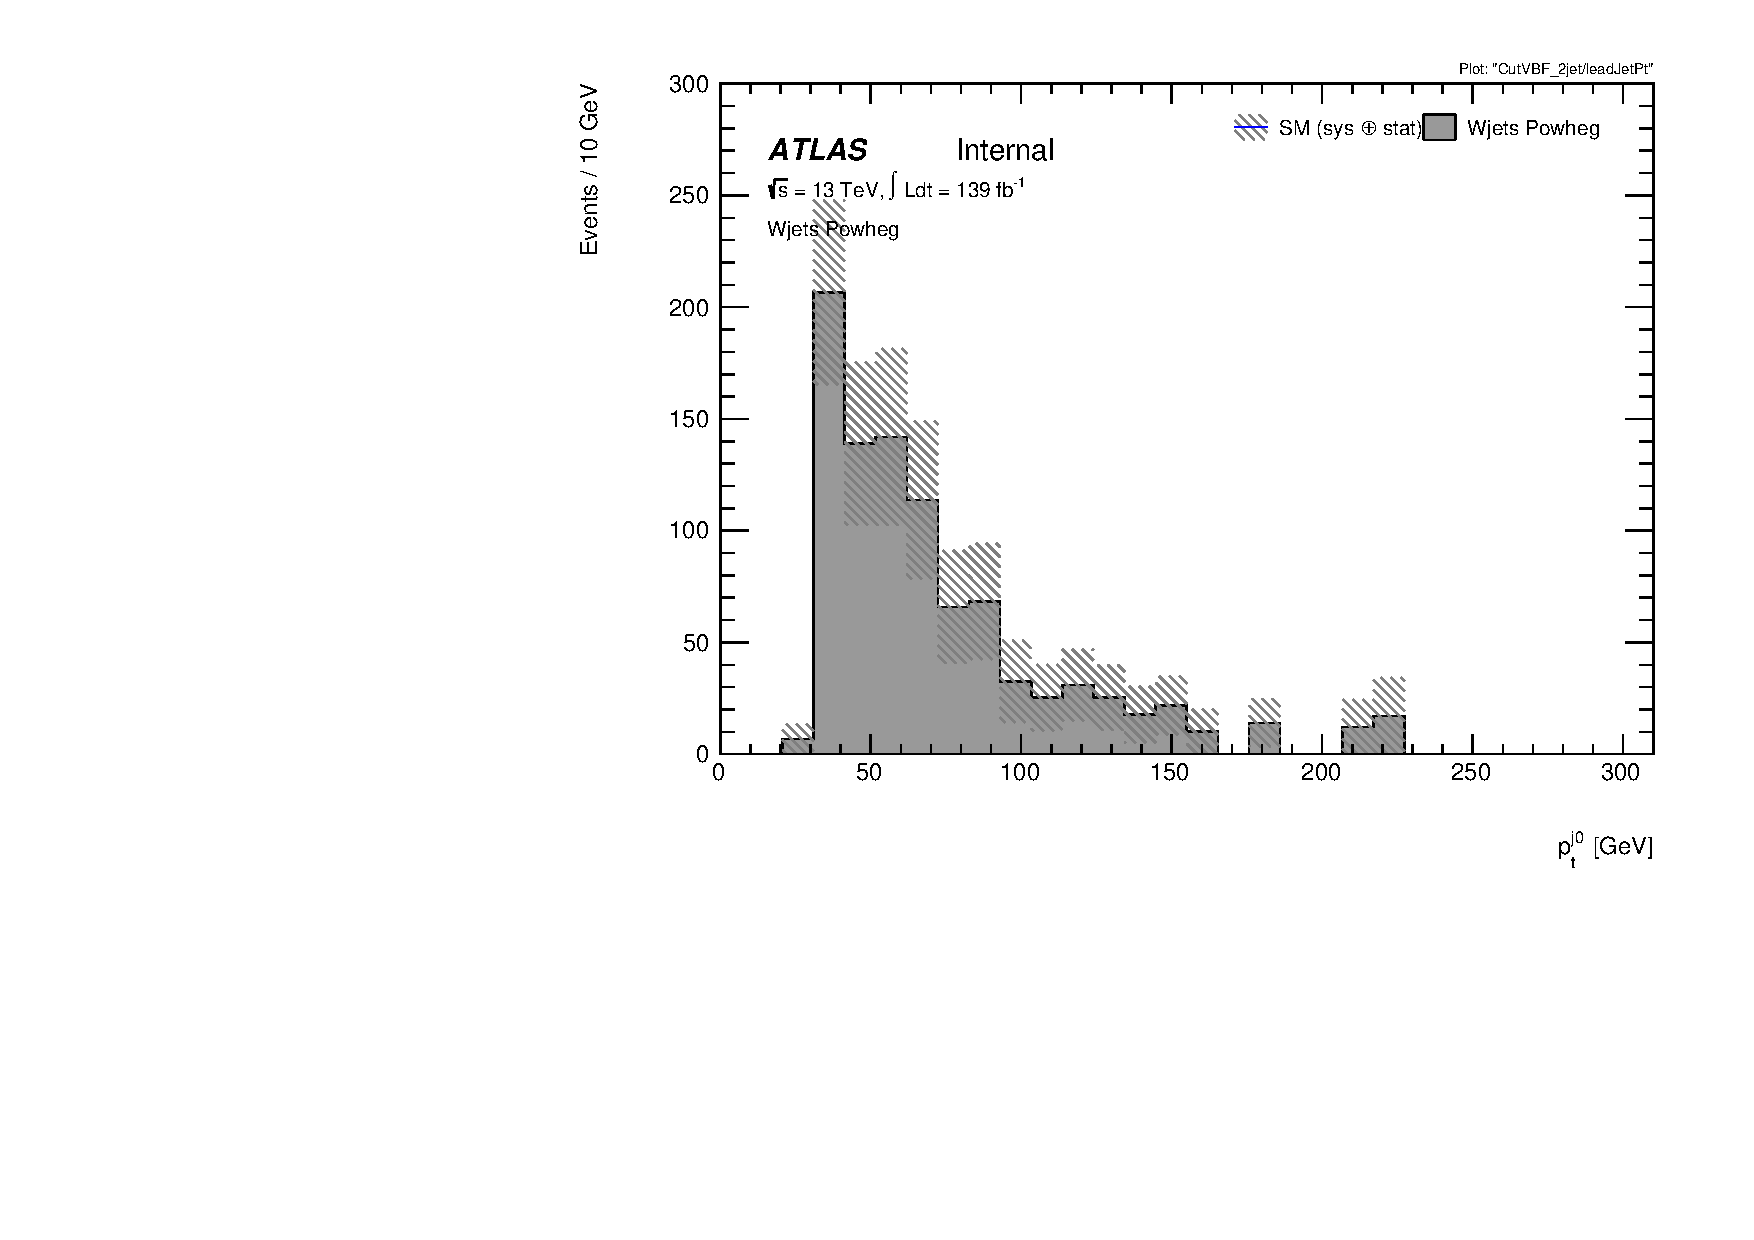
\includegraphics[width=0.3\textwidth]{FakeClosure/run2-emme-CutVBF_2jet-leadJetPt-lin.pdf}
  }\hfill
  \subfloat[$p_T^{j1}$]{
      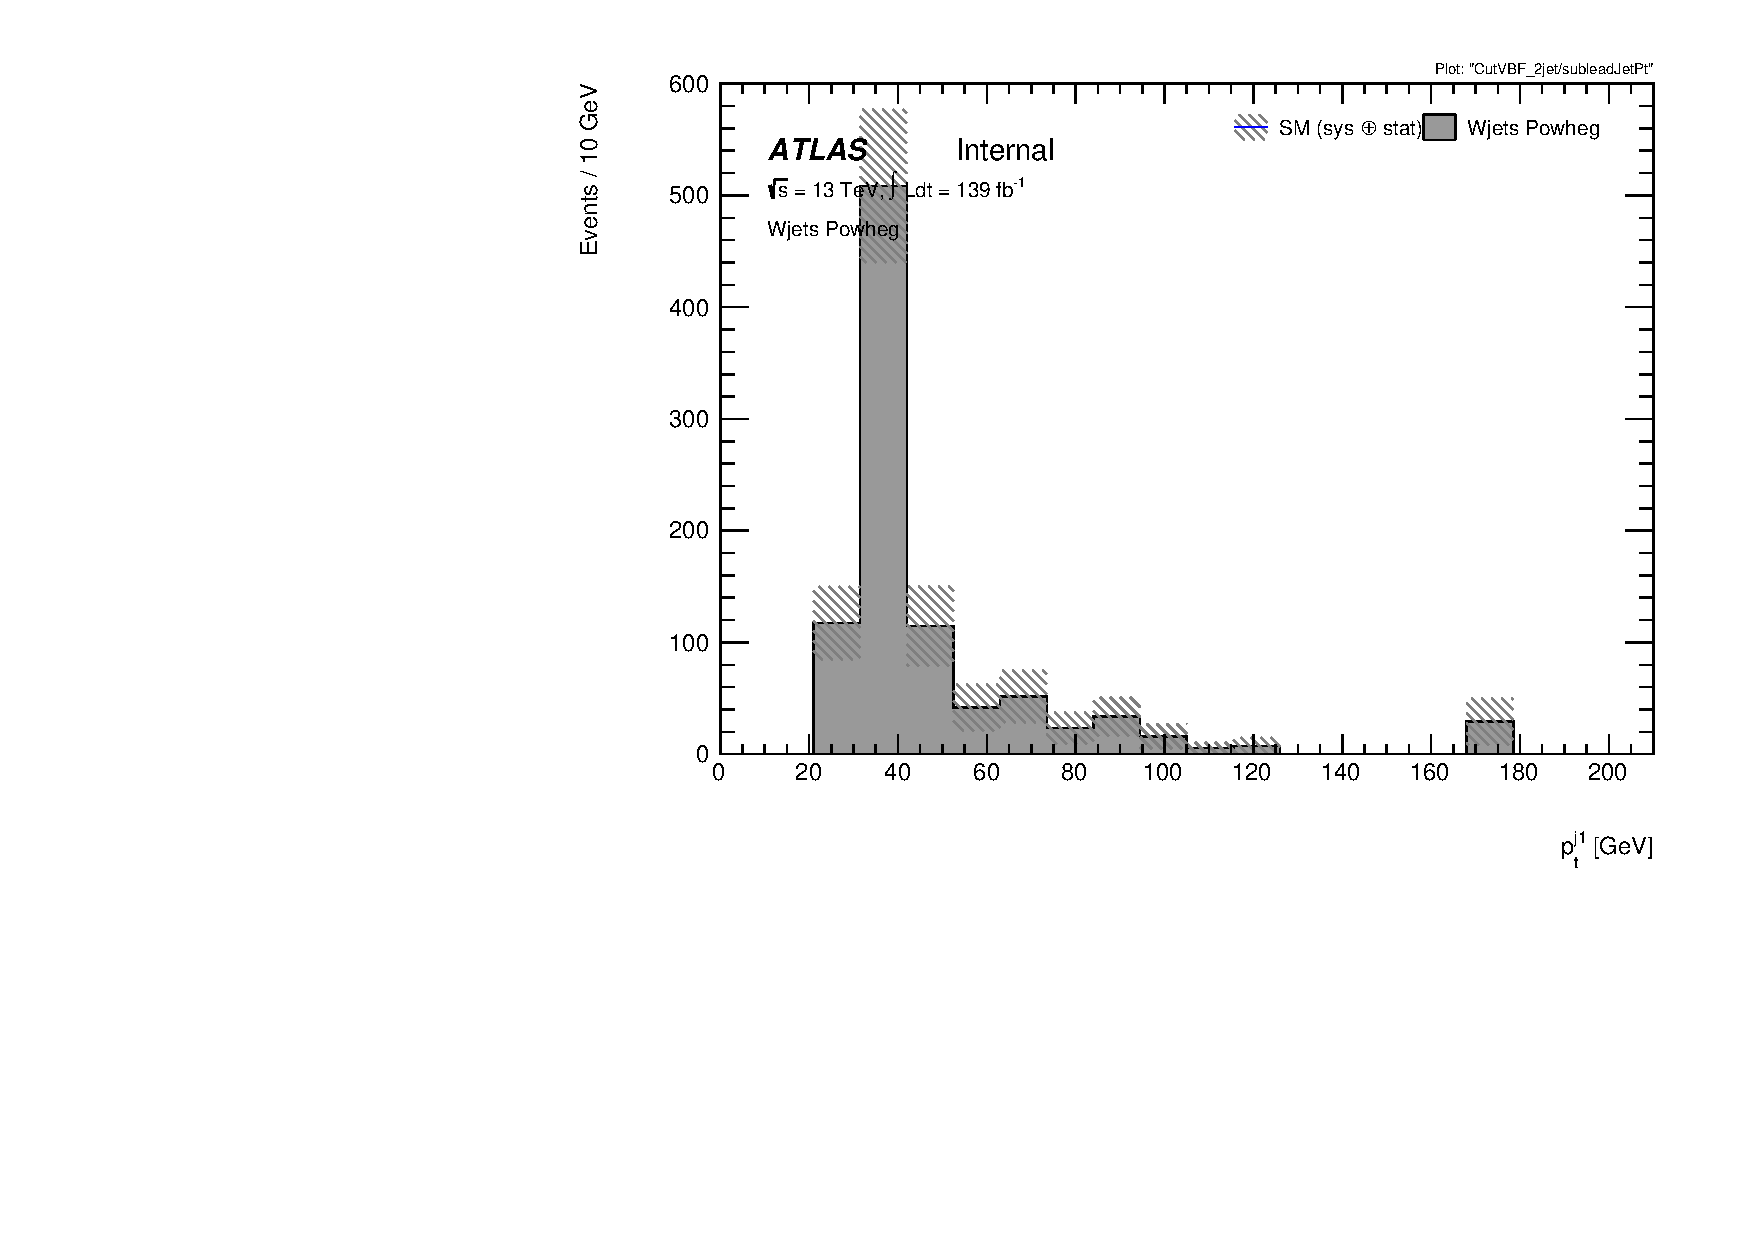
\includegraphics[width=0.3\textwidth]{FakeClosure/run2-emme-CutVBF_2jet-subleadJetPt-lin.pdf}
  }\hfill
  \subfloat[$\eta^{l0}$]{
      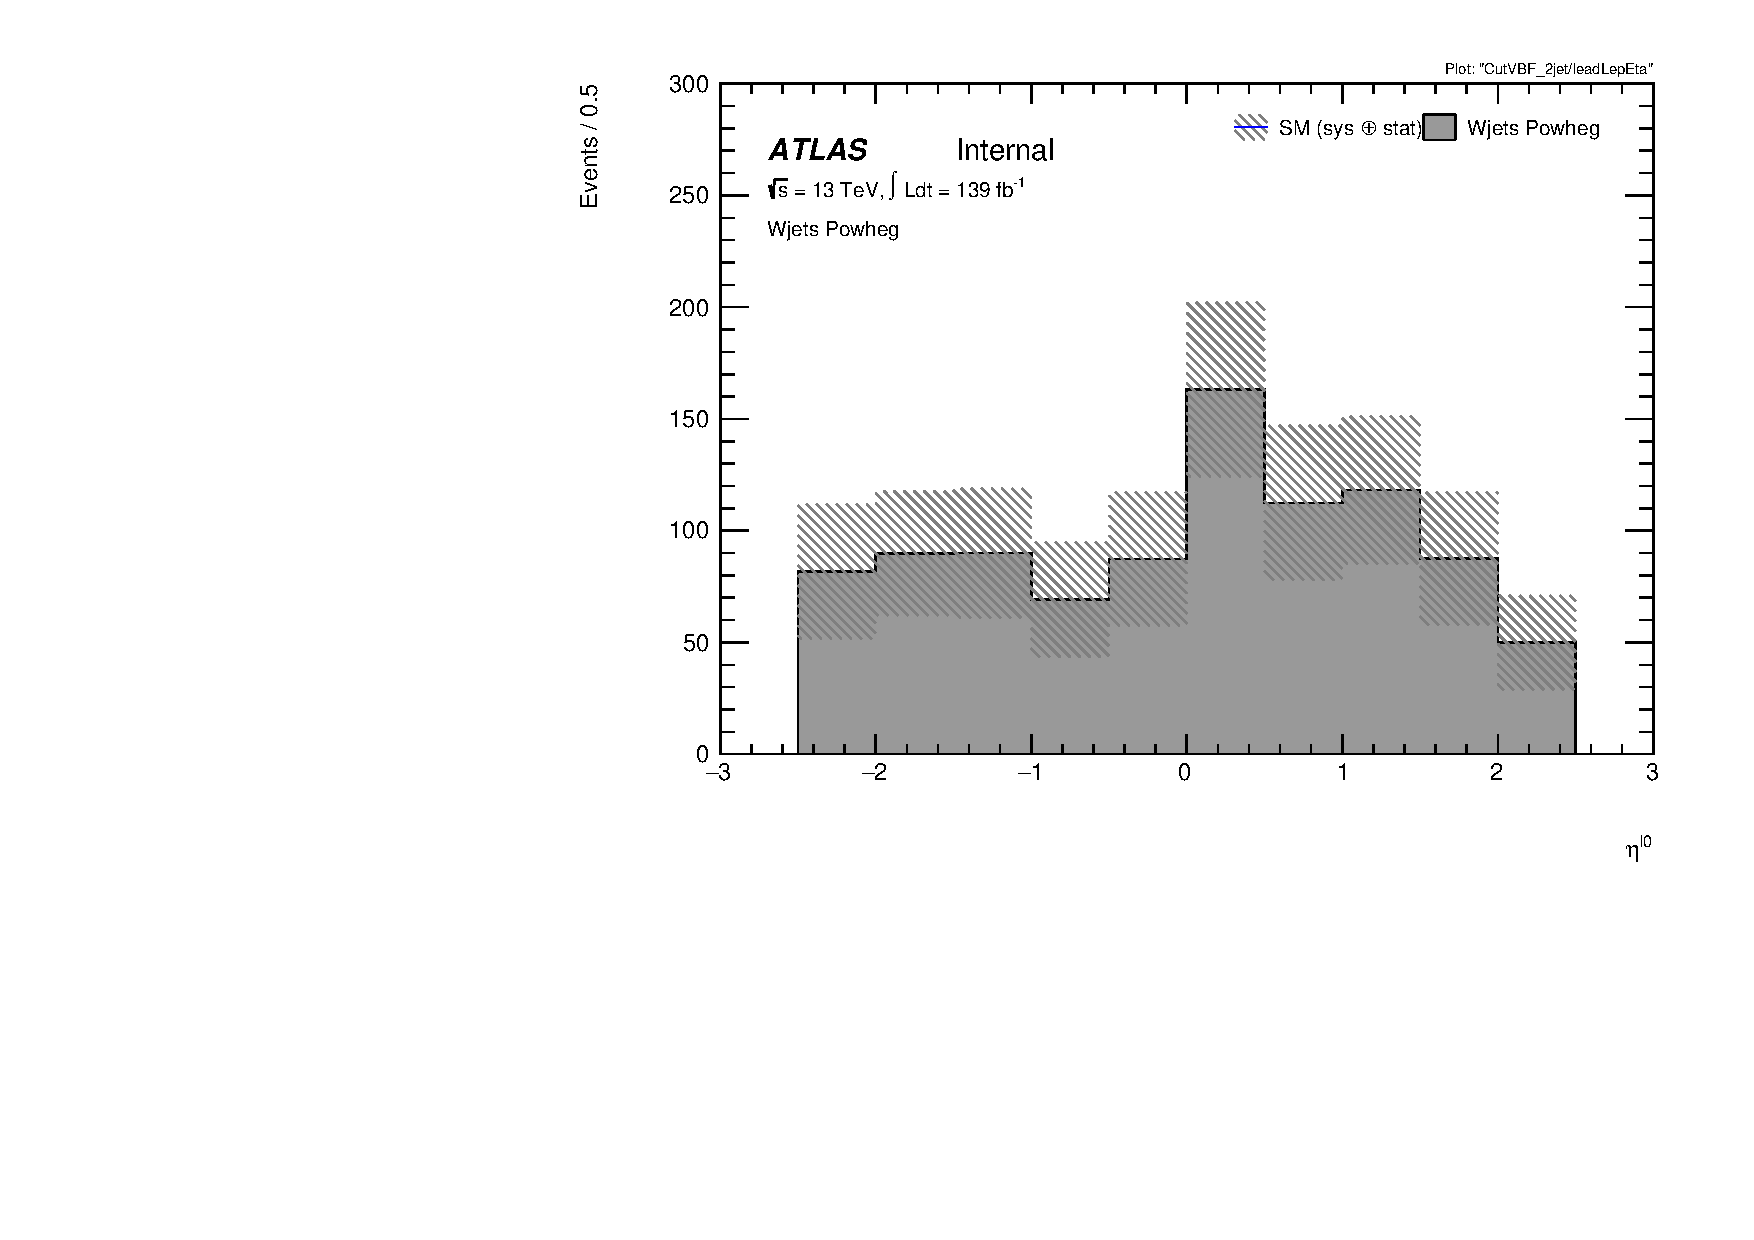
\includegraphics[width=0.23\textwidth]{FakeClosure/run2-emme-CutVBF_2jet-leadLepEta-lin.pdf}
  }\hfill
  \subfloat[$\eta^{l1}$]{
      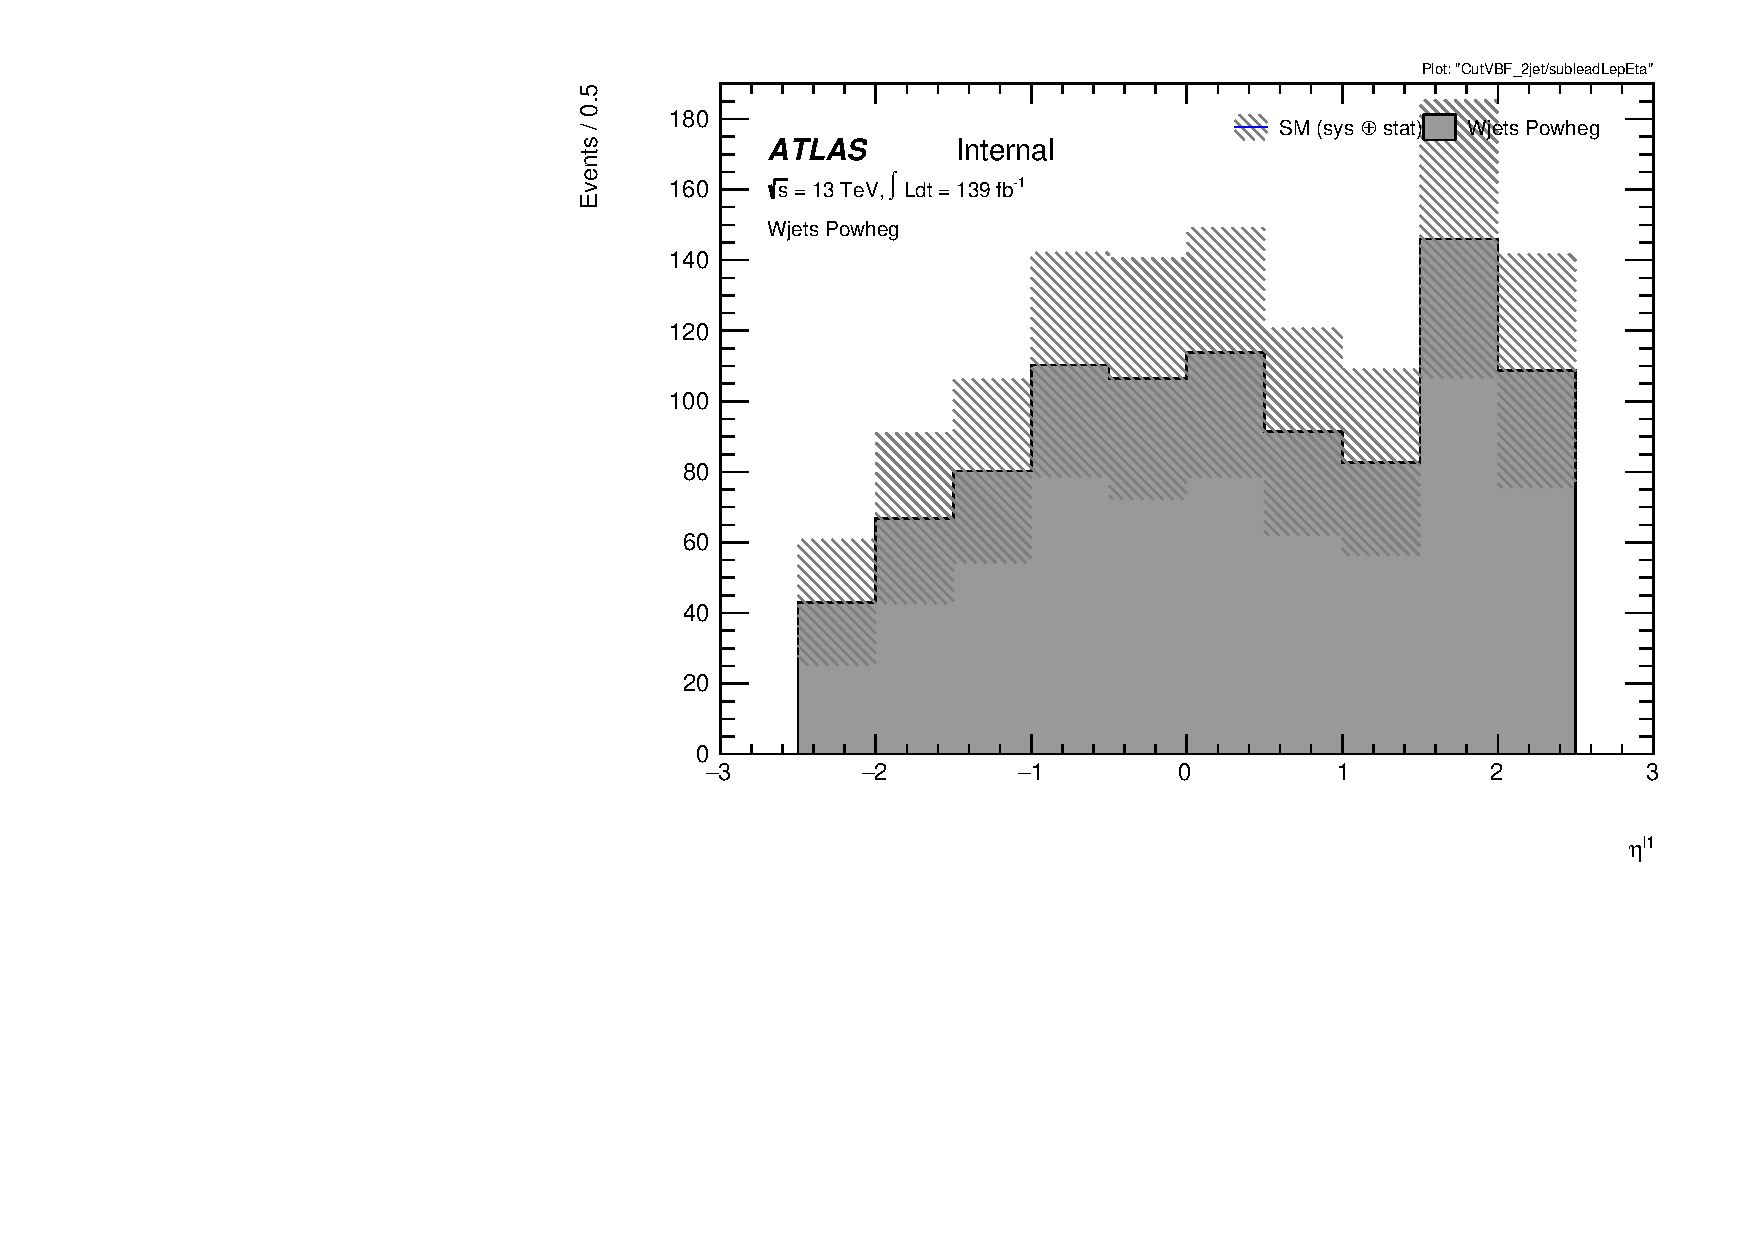
\includegraphics[width=0.23\textwidth]{FakeClosure/run2-emme-CutVBF_2jet-subleadLepEta-lin.pdf}
  }\hfill
  \subfloat[$\eta^{j0}$]{
      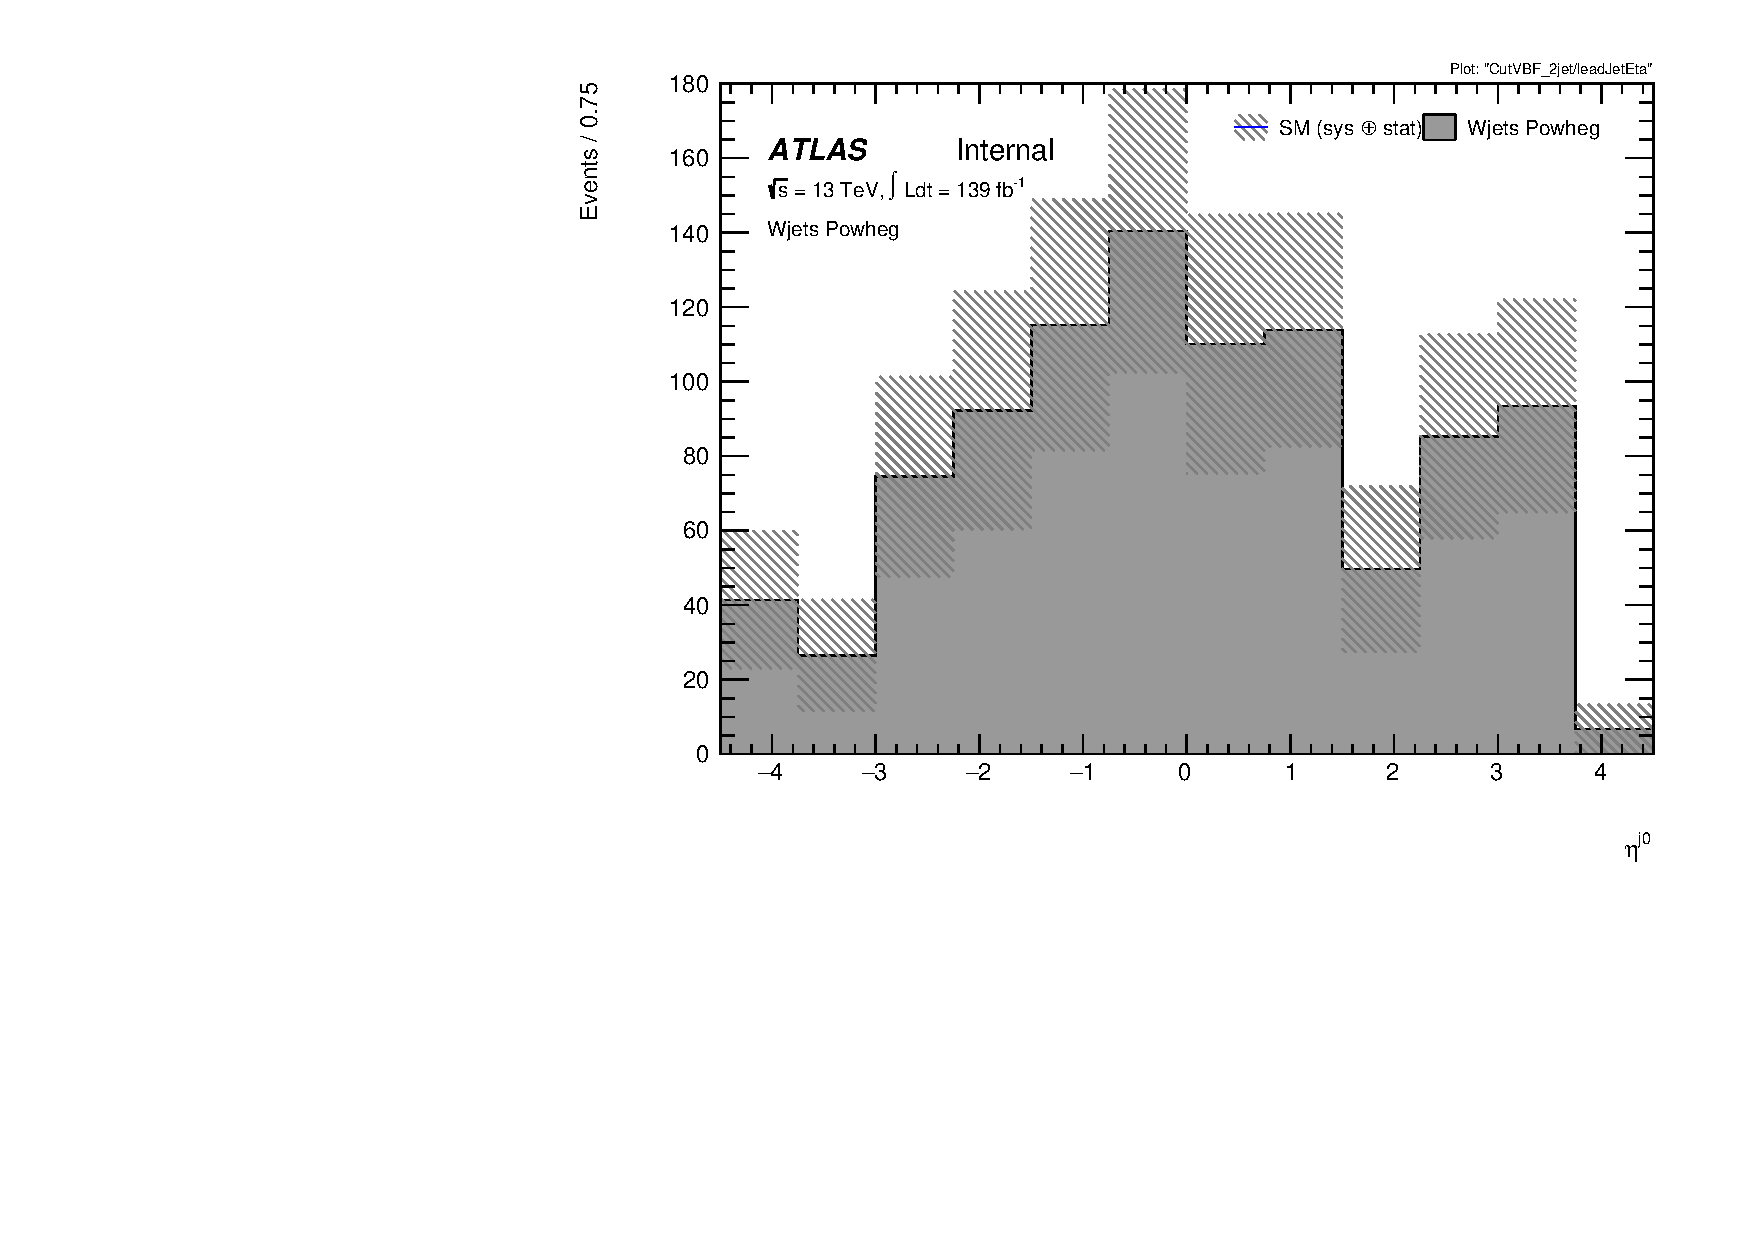
\includegraphics[width=0.23\textwidth]{FakeClosure/run2-emme-CutVBF_2jet-leadJetEta-lin.pdf}
  }\hfill
  \subfloat[$\eta^{j1}$]{
      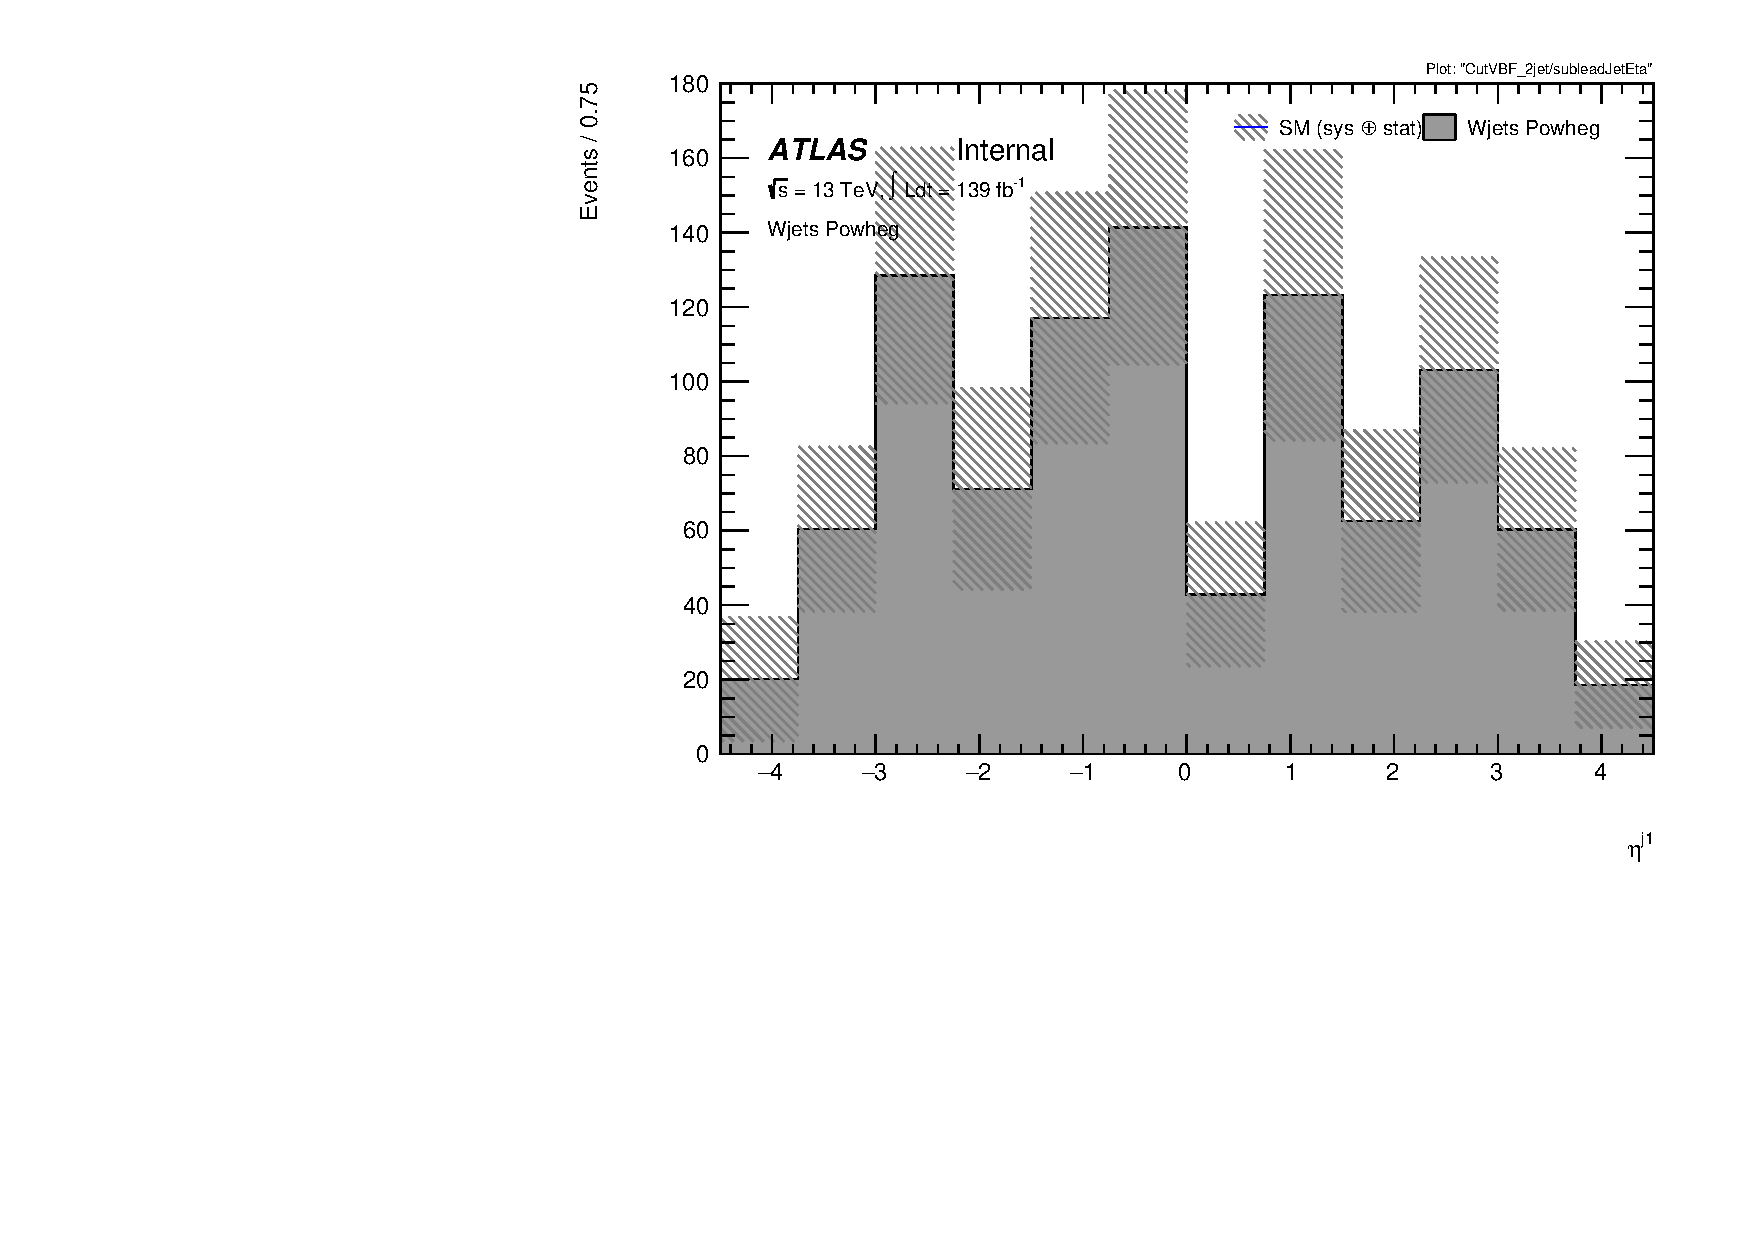
\includegraphics[width=0.23\textwidth]{FakeClosure/run2-emme-CutVBF_2jet-subleadJetEta-lin.pdf}
  }%\hfill
{\caption{Distributions after preselection and 2-jets cuts for $W+$jets MC samples in the signal region (id-id).
\label{fig:SR2jet}}}
\end{figure}


\begin{figure}[!h]
\centering
  \subfloat[$m_{jj}$]{
      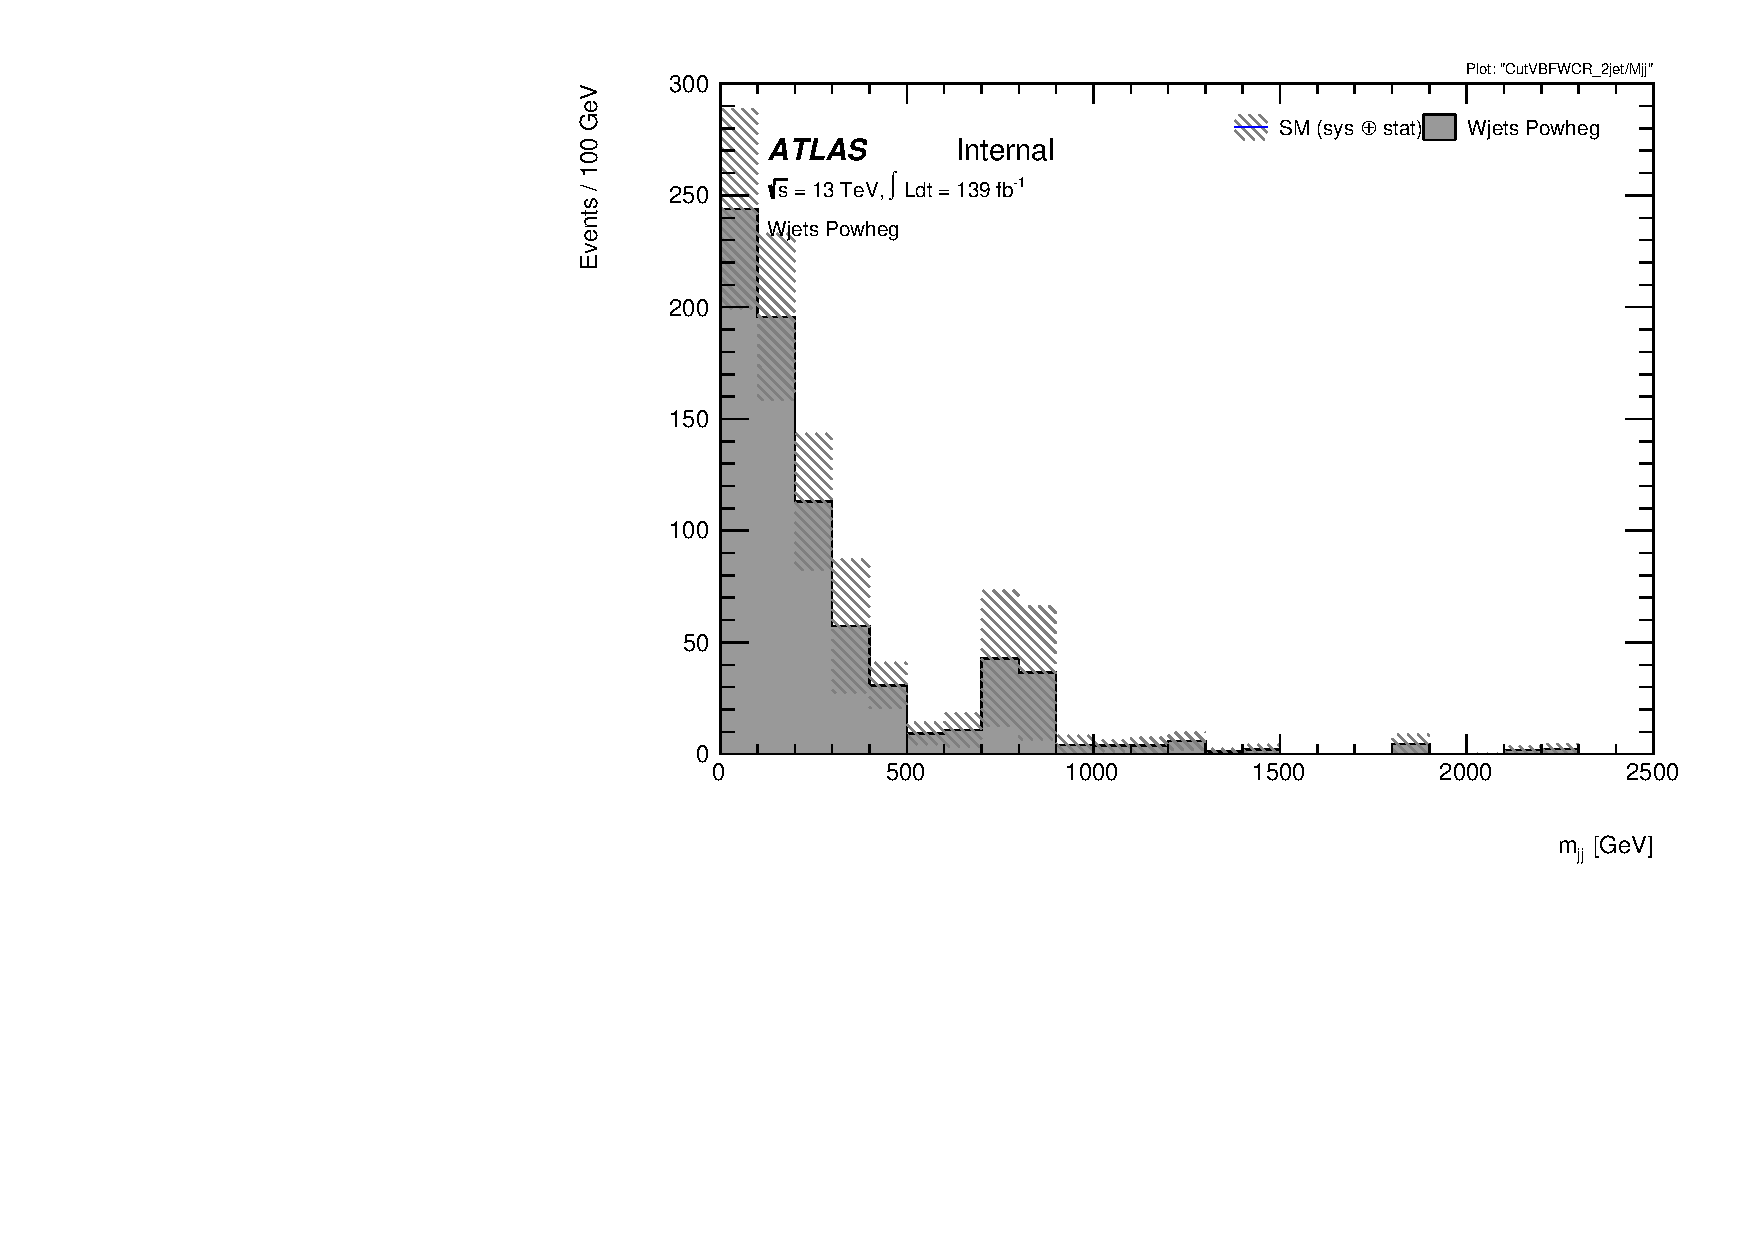
\includegraphics[width=0.3\textwidth]{FakeClosure/run2-emme-CutVBFWCR_2jet-Mjj-lin.pdf}
  }\hfill
  \subfloat[$p^H_{T}$]{
      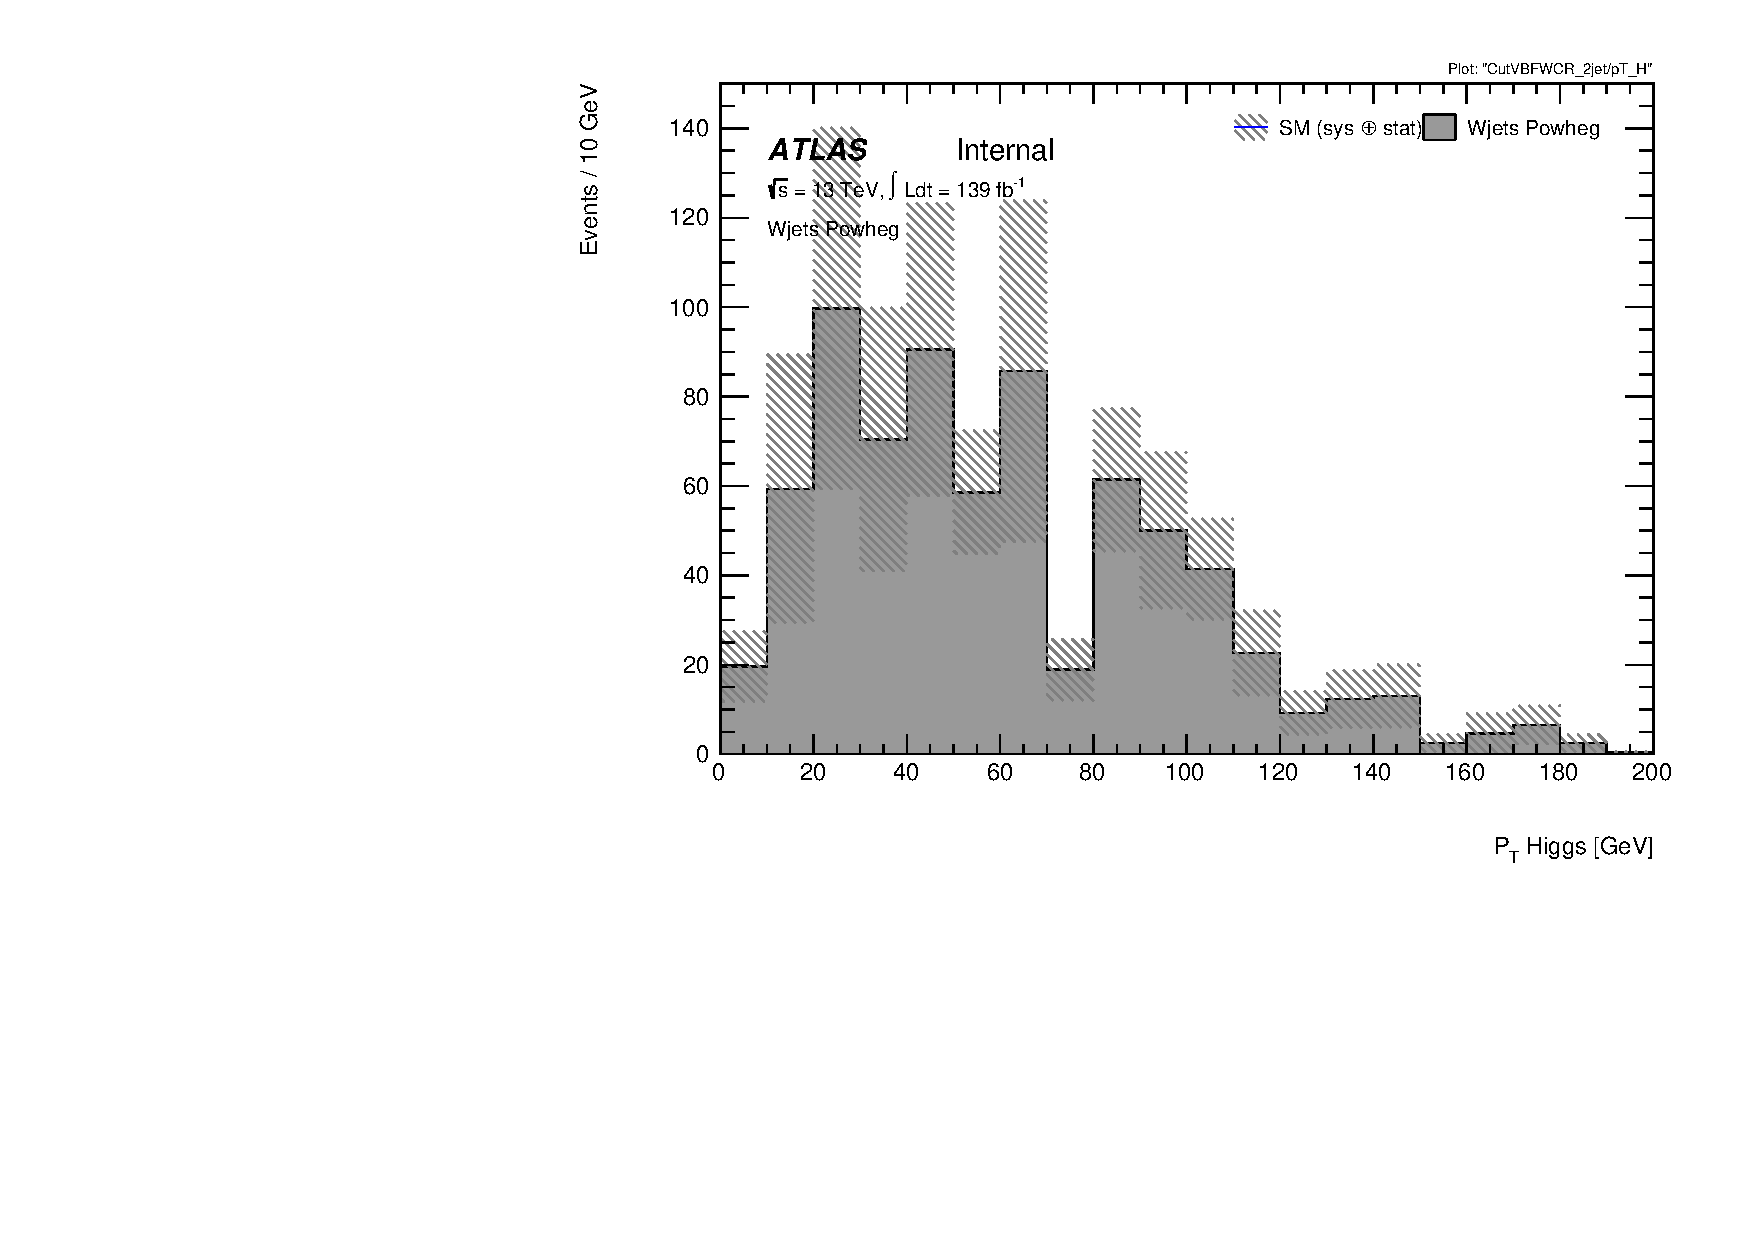
\includegraphics[width=0.3\textwidth]{FakeClosure/run2-emme-CutVBFWCR_2jet-pT_H-lin.pdf}
  }\hfill
  \subfloat[$p_T^{l0}$]{
      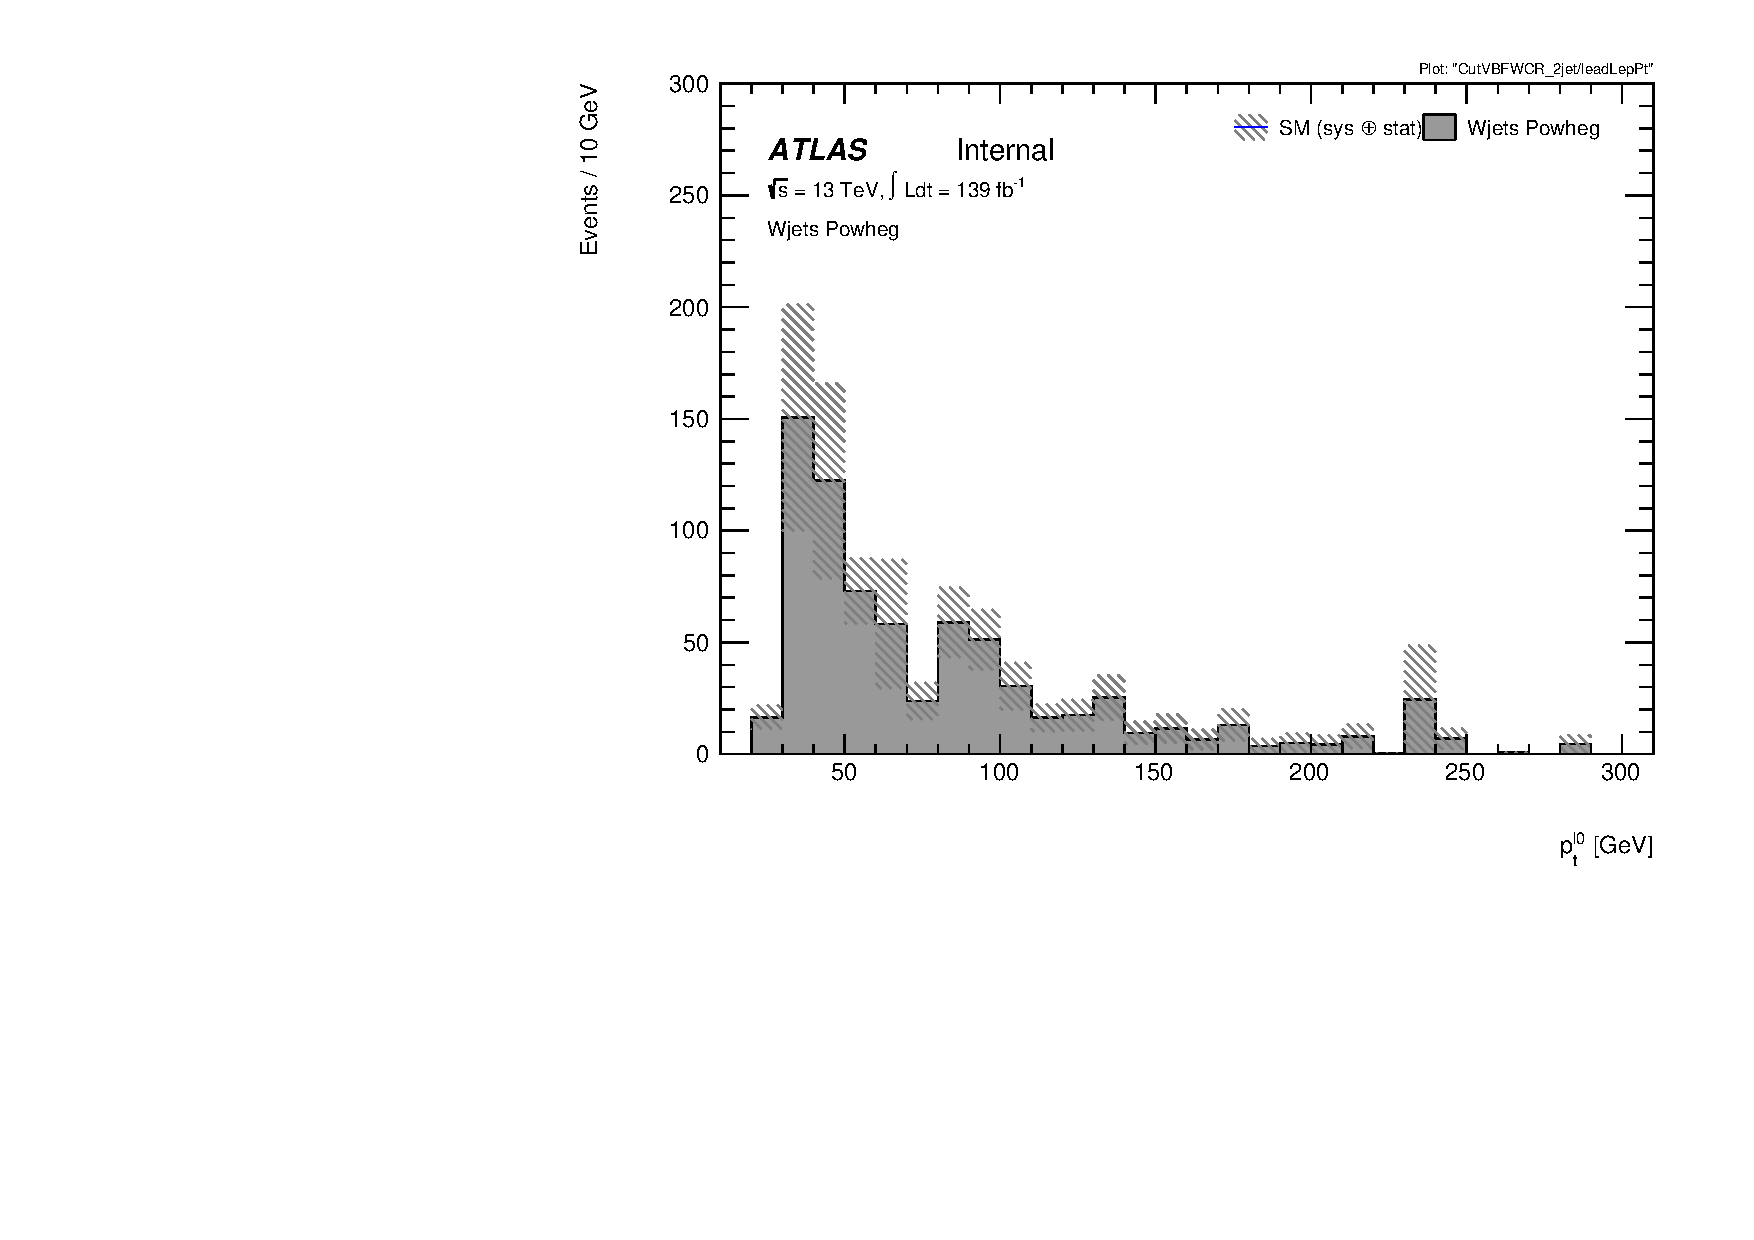
\includegraphics[width=0.3\textwidth]{FakeClosure/run2-emme-CutVBFWCR_2jet-leadLepPt-lin.pdf}
  }\hfill
  \subfloat[$p_T^{l1}$]{
      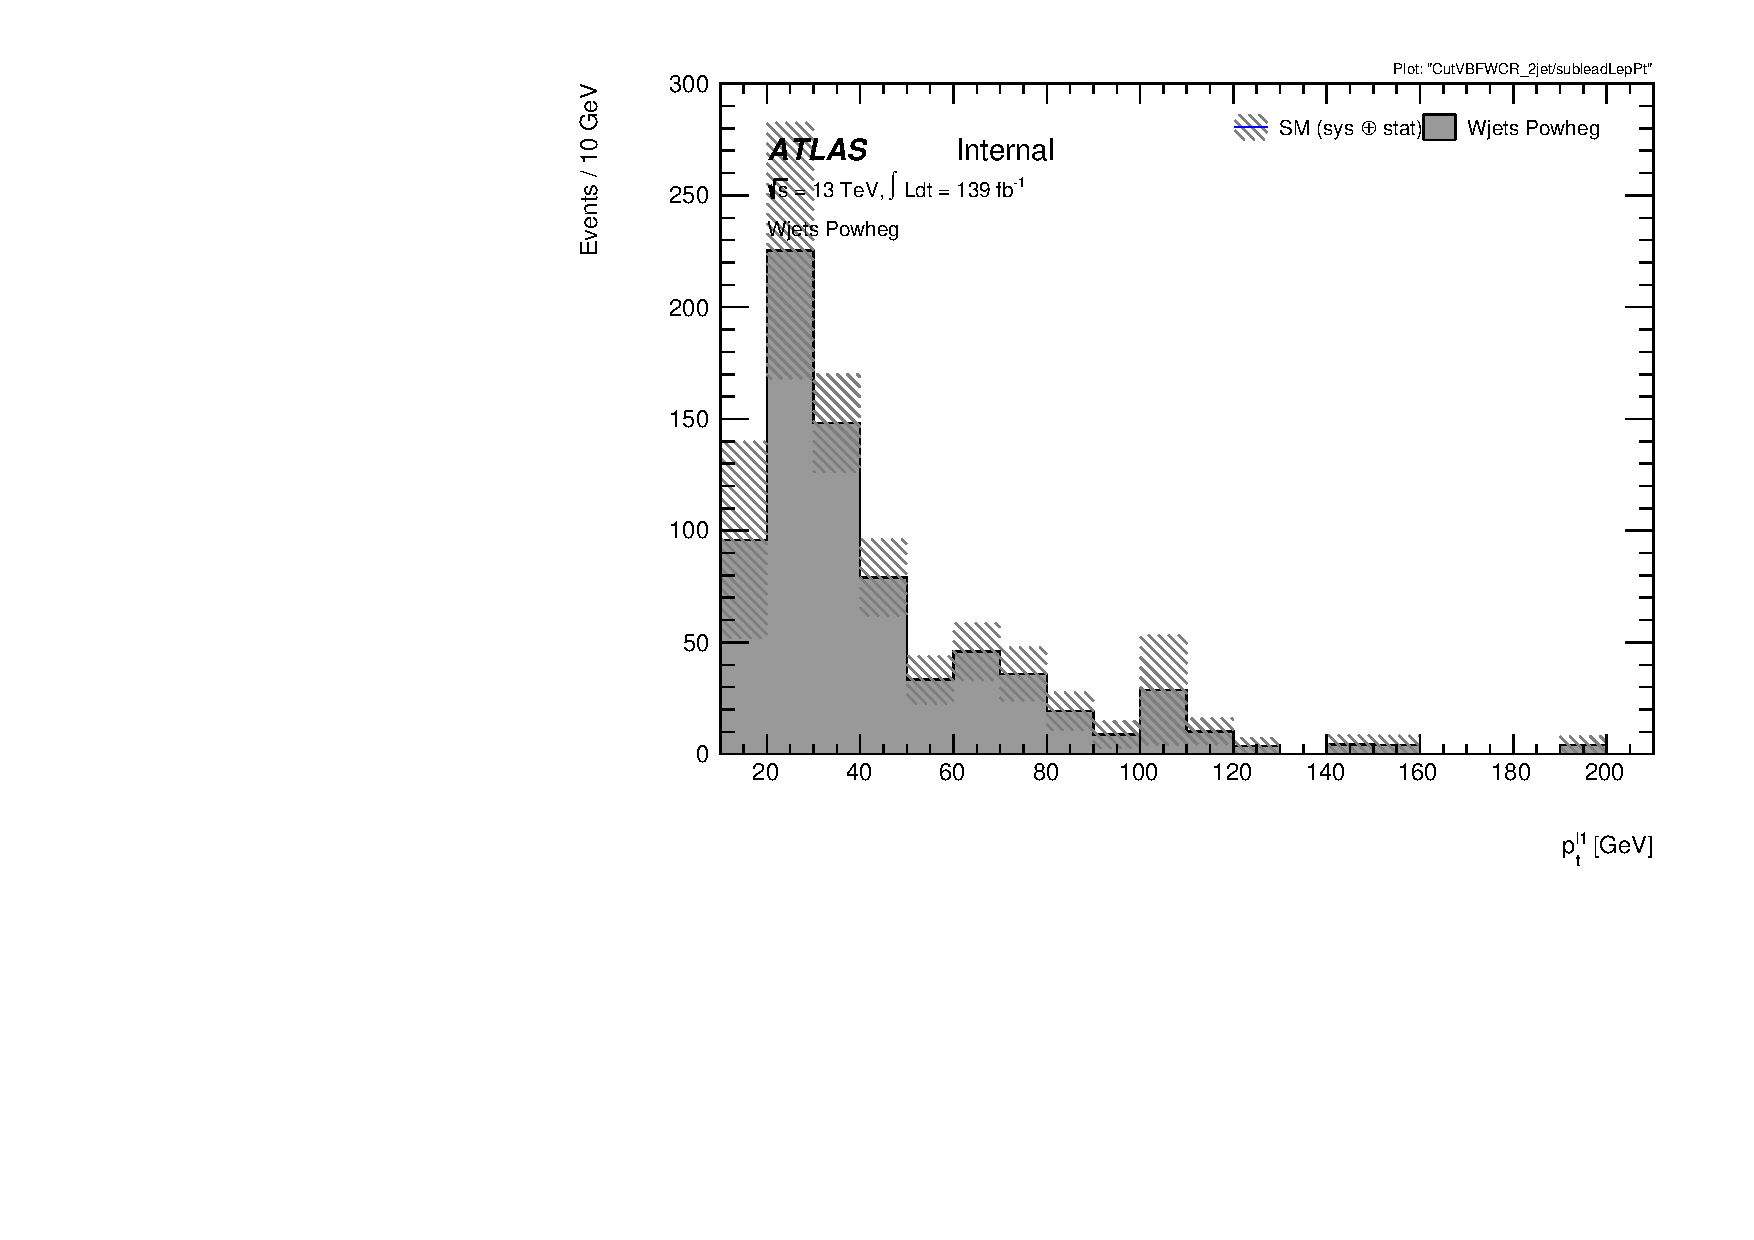
\includegraphics[width=0.3\textwidth]{FakeClosure/run2-emme-CutVBFWCR_2jet-subleadLepPt-lin.pdf}
  }\hfill
  \subfloat[$p_T^{j0}$]{
      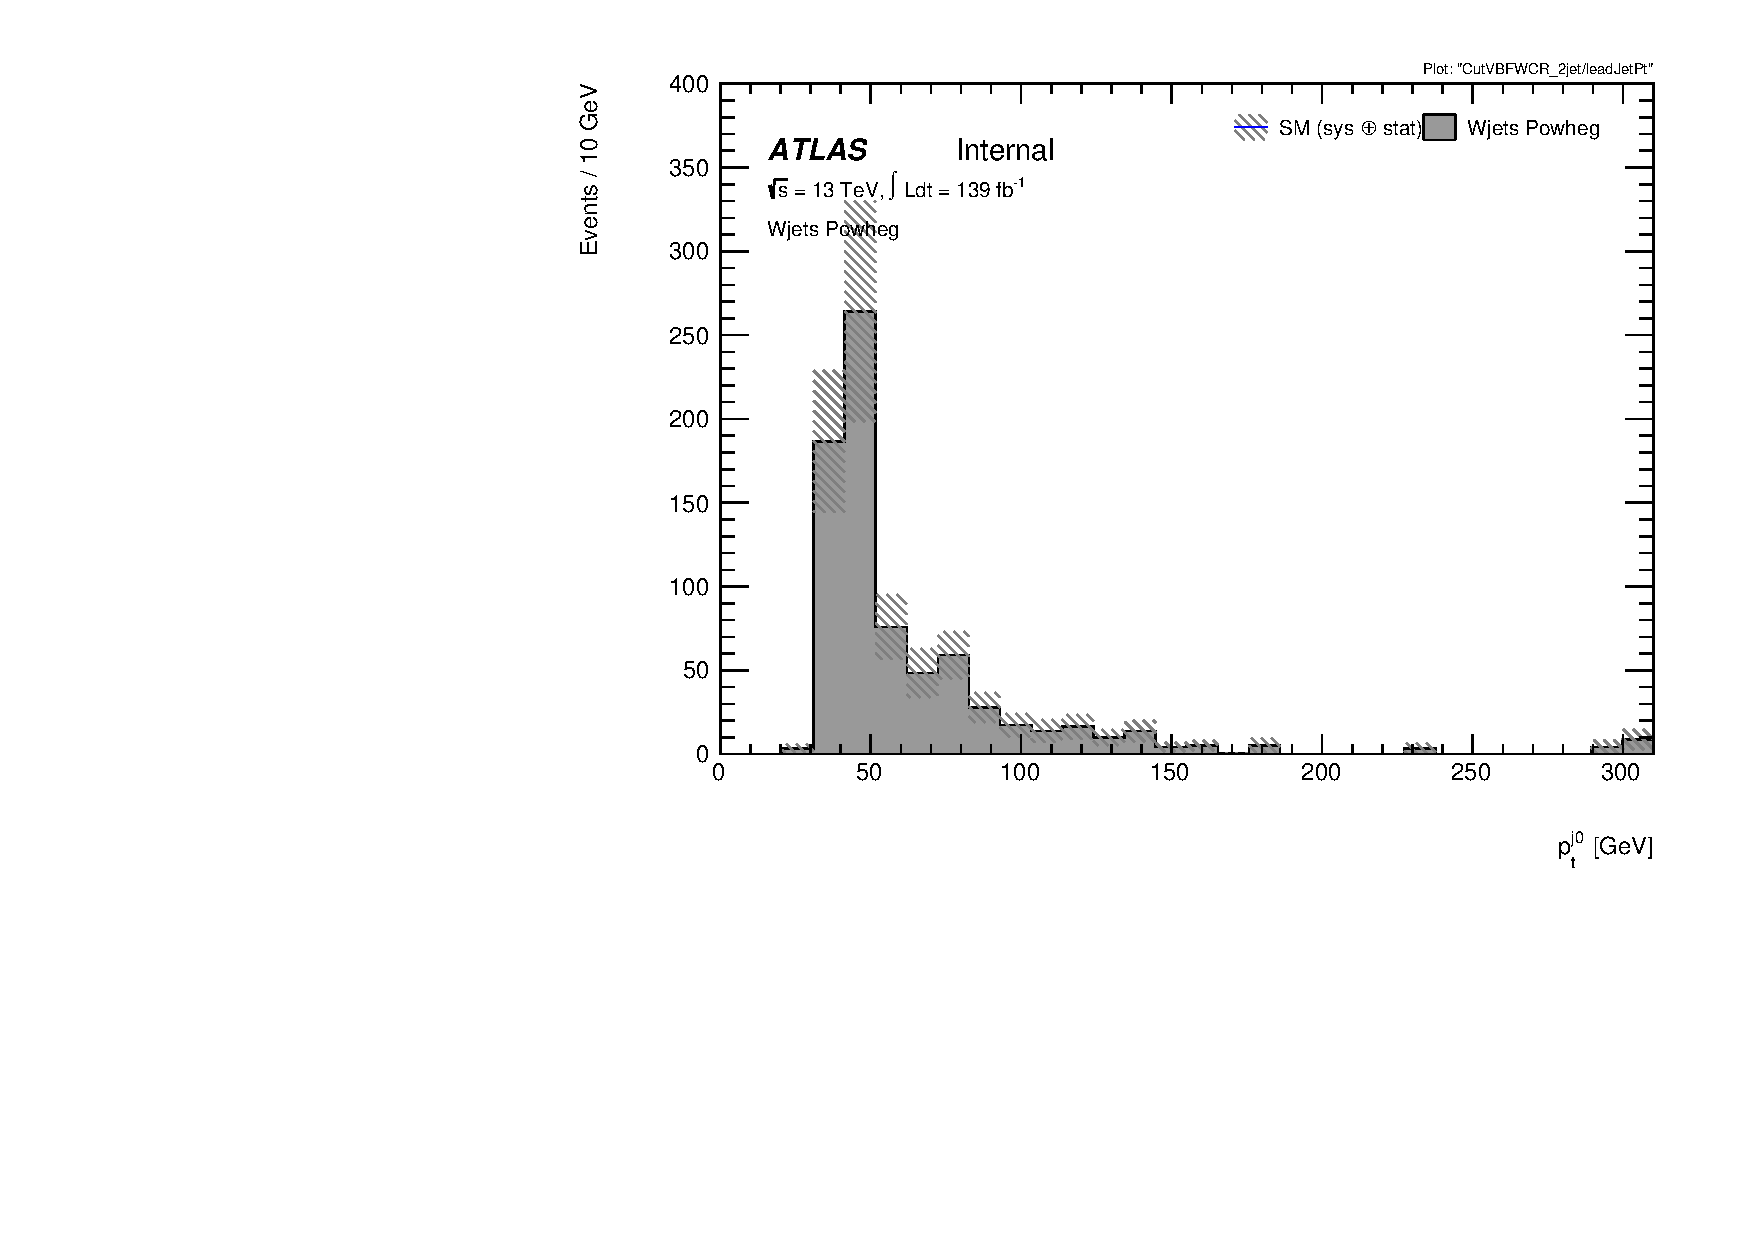
\includegraphics[width=0.3\textwidth]{FakeClosure/run2-emme-CutVBFWCR_2jet-leadJetPt-lin.pdf}
  }\hfill
  \subfloat[$p_T^{j1}$]{
      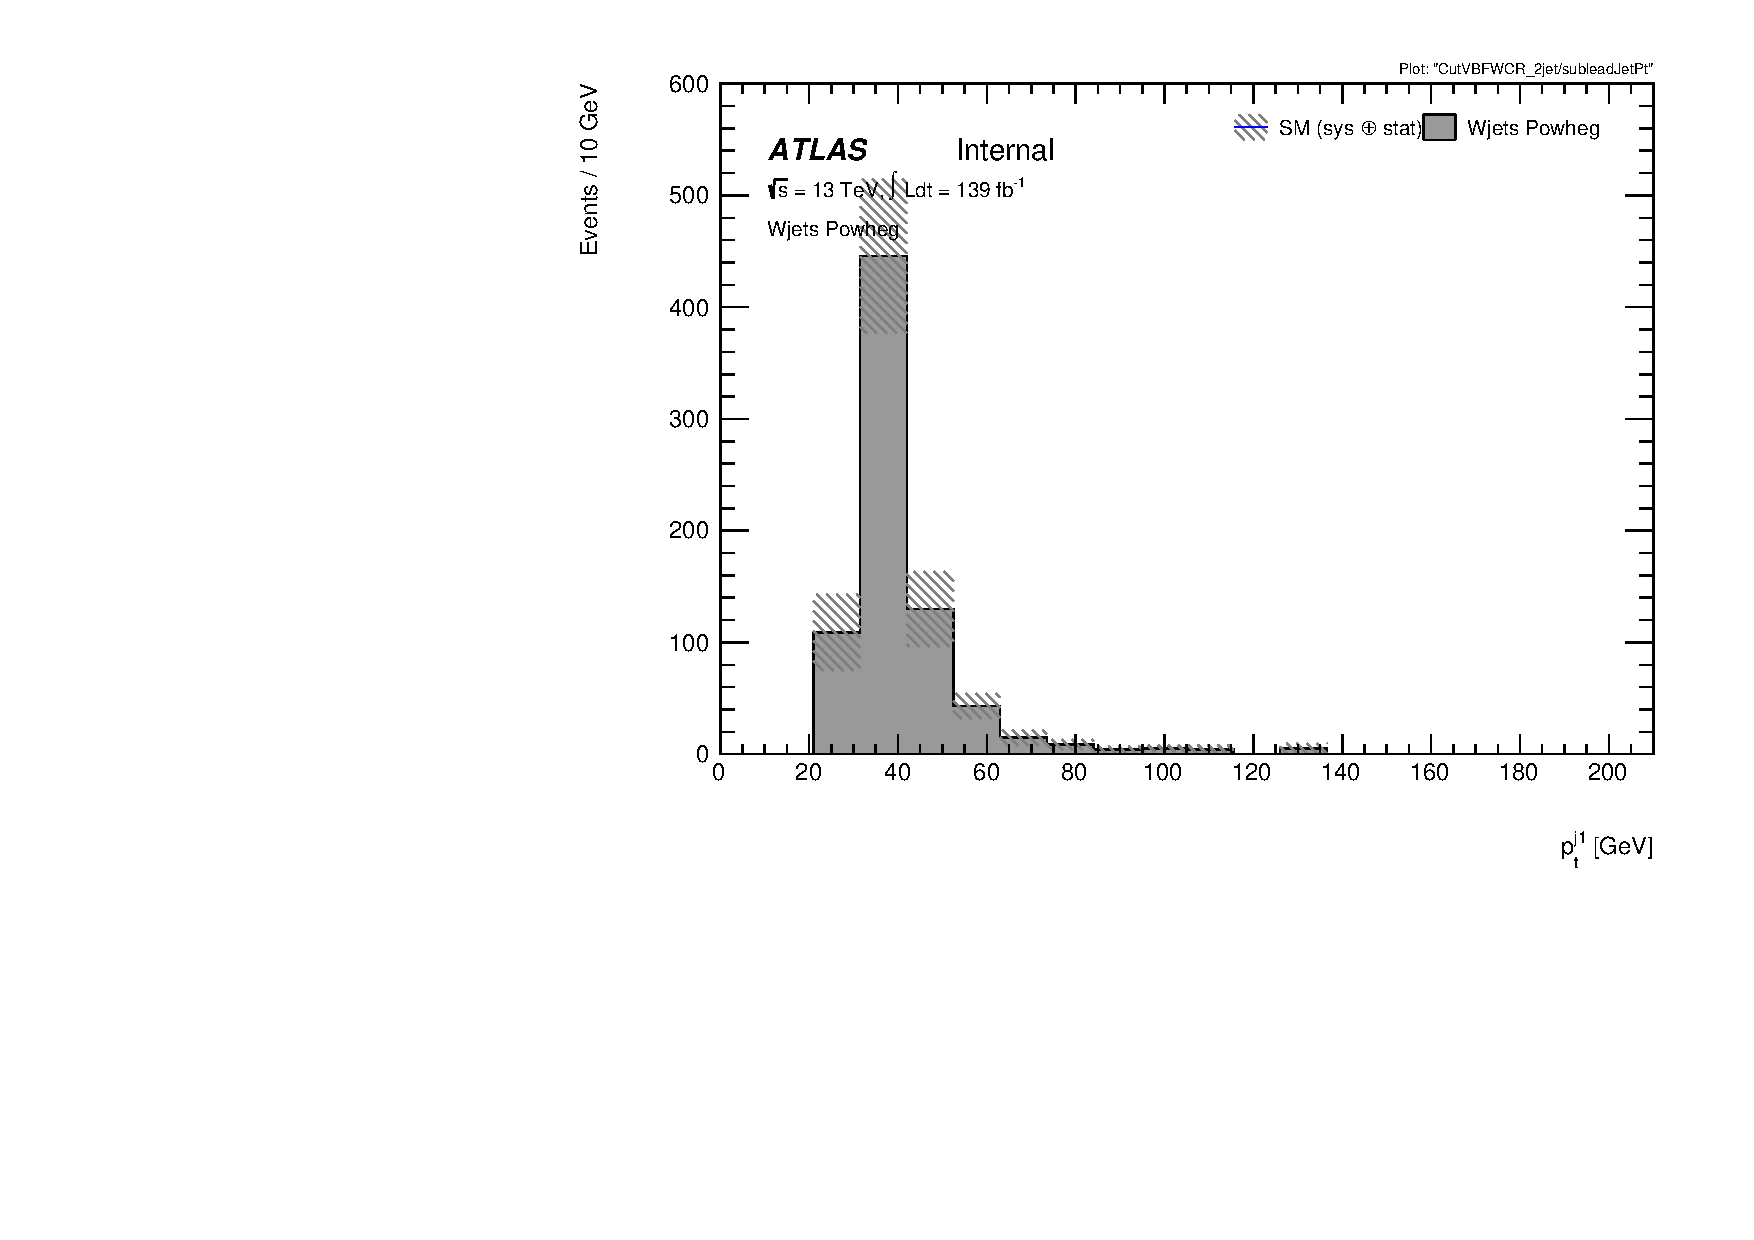
\includegraphics[width=0.3\textwidth]{FakeClosure/run2-emme-CutVBFWCR_2jet-subleadJetPt-lin.pdf}
  }\hfill
  \subfloat[$\eta^{l0}$]{
      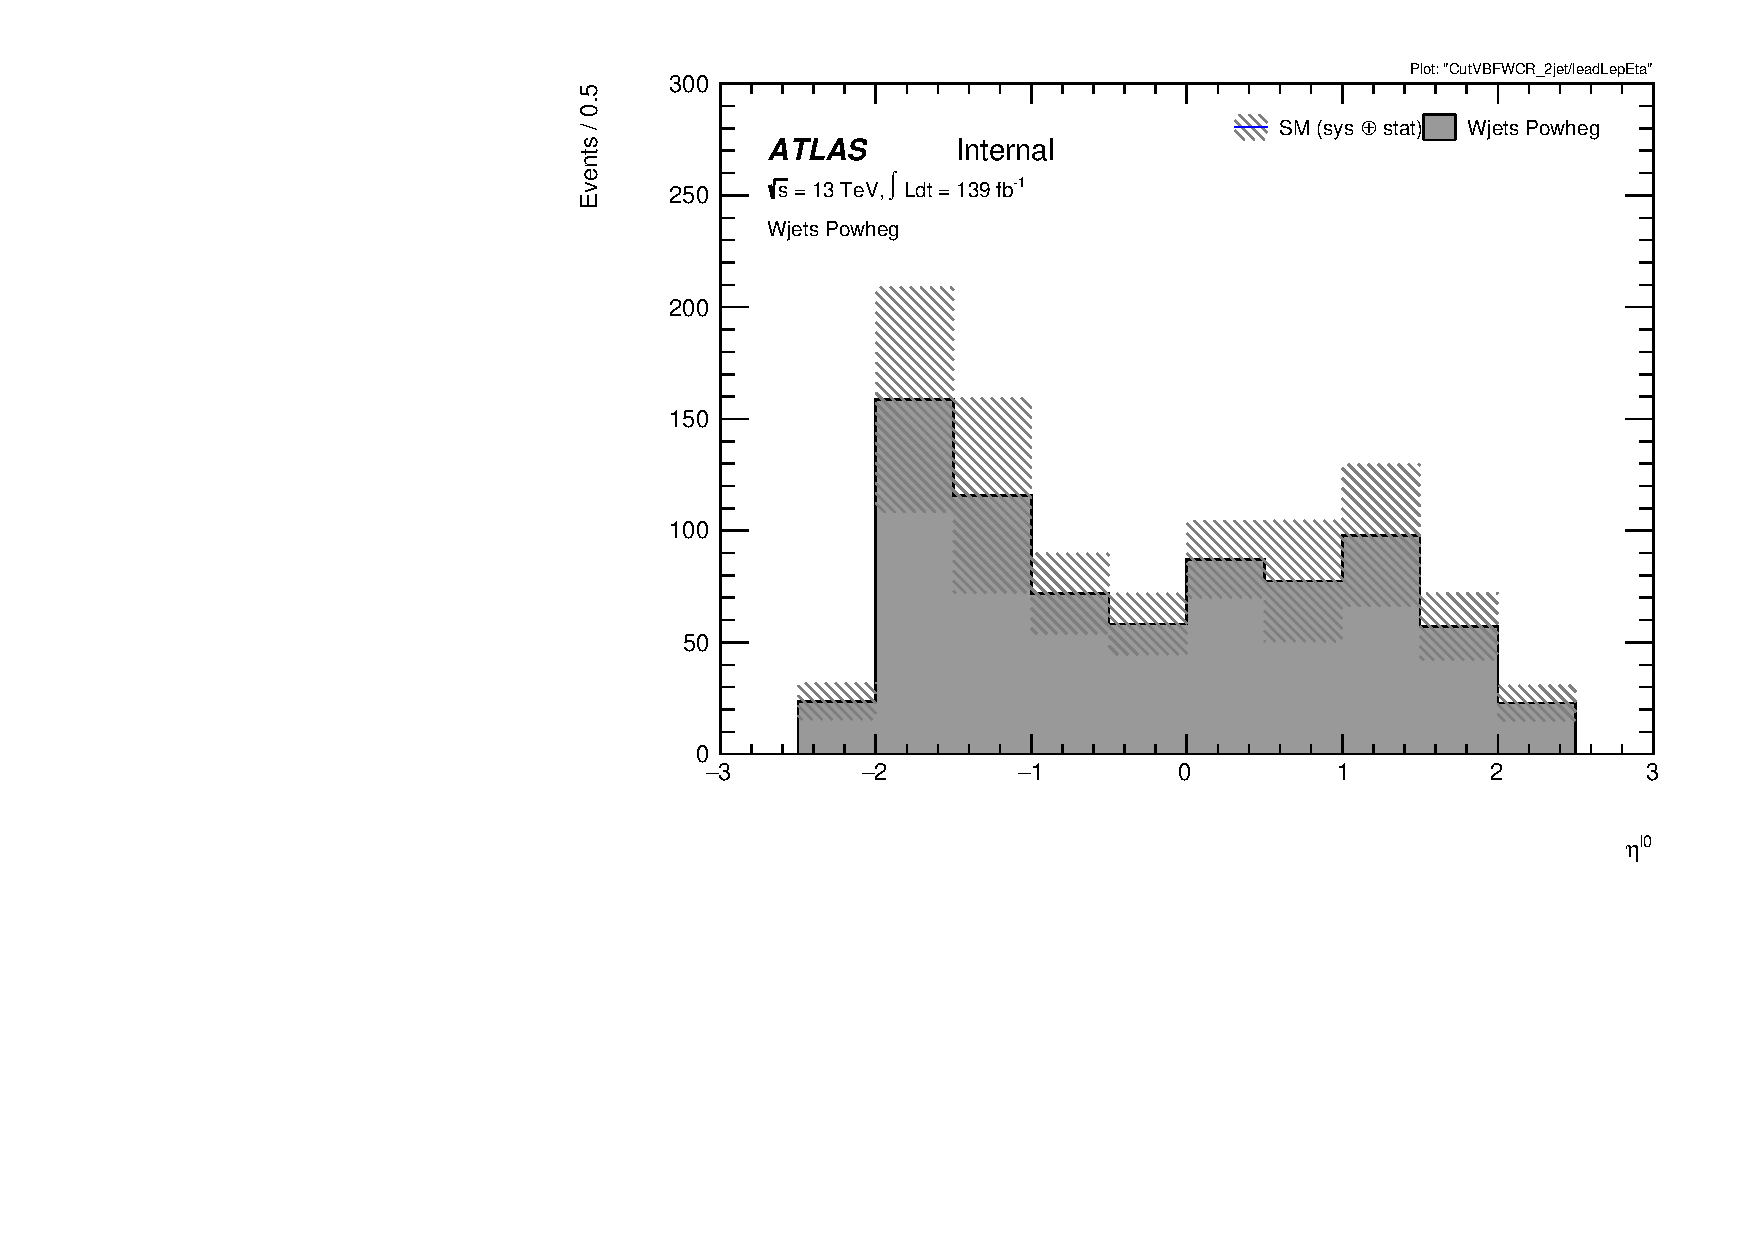
\includegraphics[width=0.23\textwidth]{FakeClosure/run2-emme-CutVBFWCR_2jet-leadLepEta-lin.pdf}
  }\hfill
  \subfloat[$\eta^{l1}$]{
      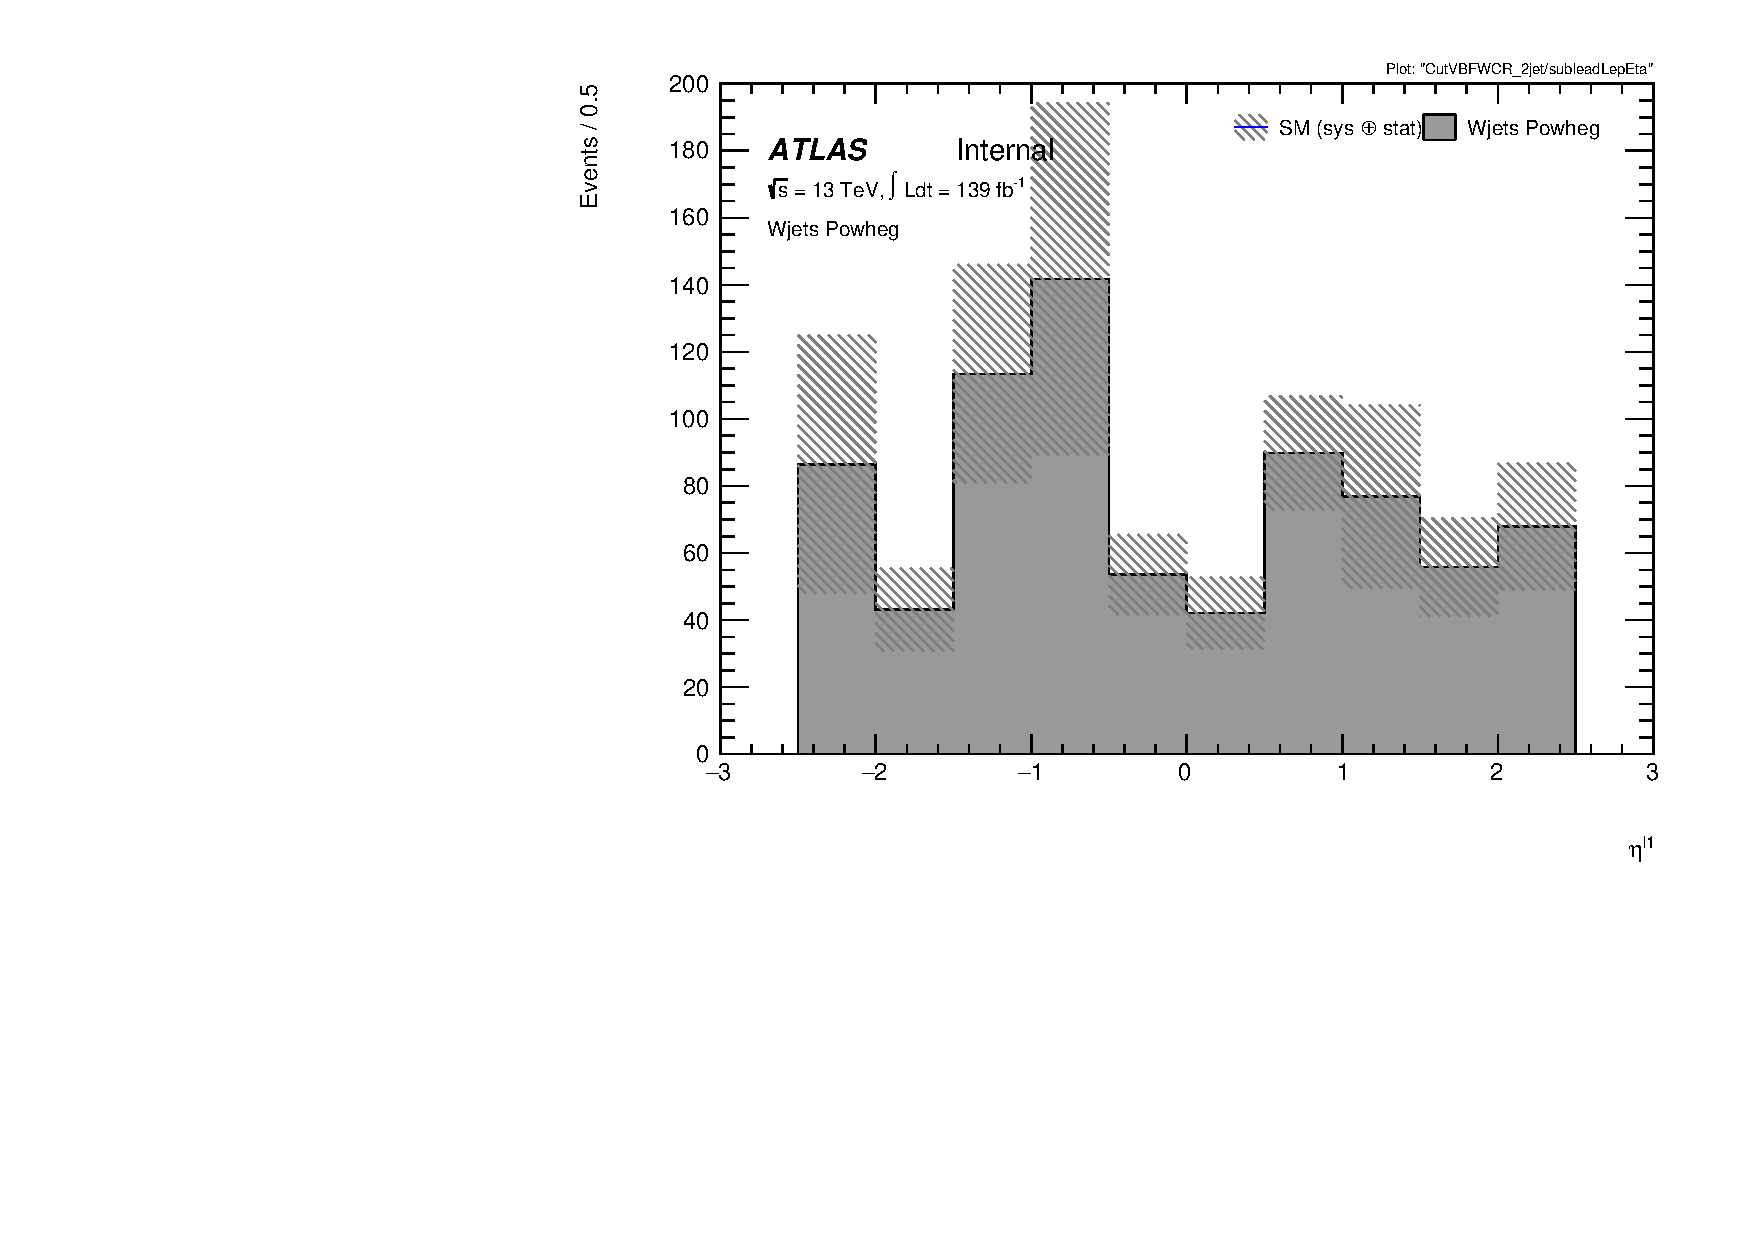
\includegraphics[width=0.23\textwidth]{FakeClosure/run2-emme-CutVBFWCR_2jet-subleadLepEta-lin.pdf}
  }\hfill
  \subfloat[$\eta^{j0}$]{
      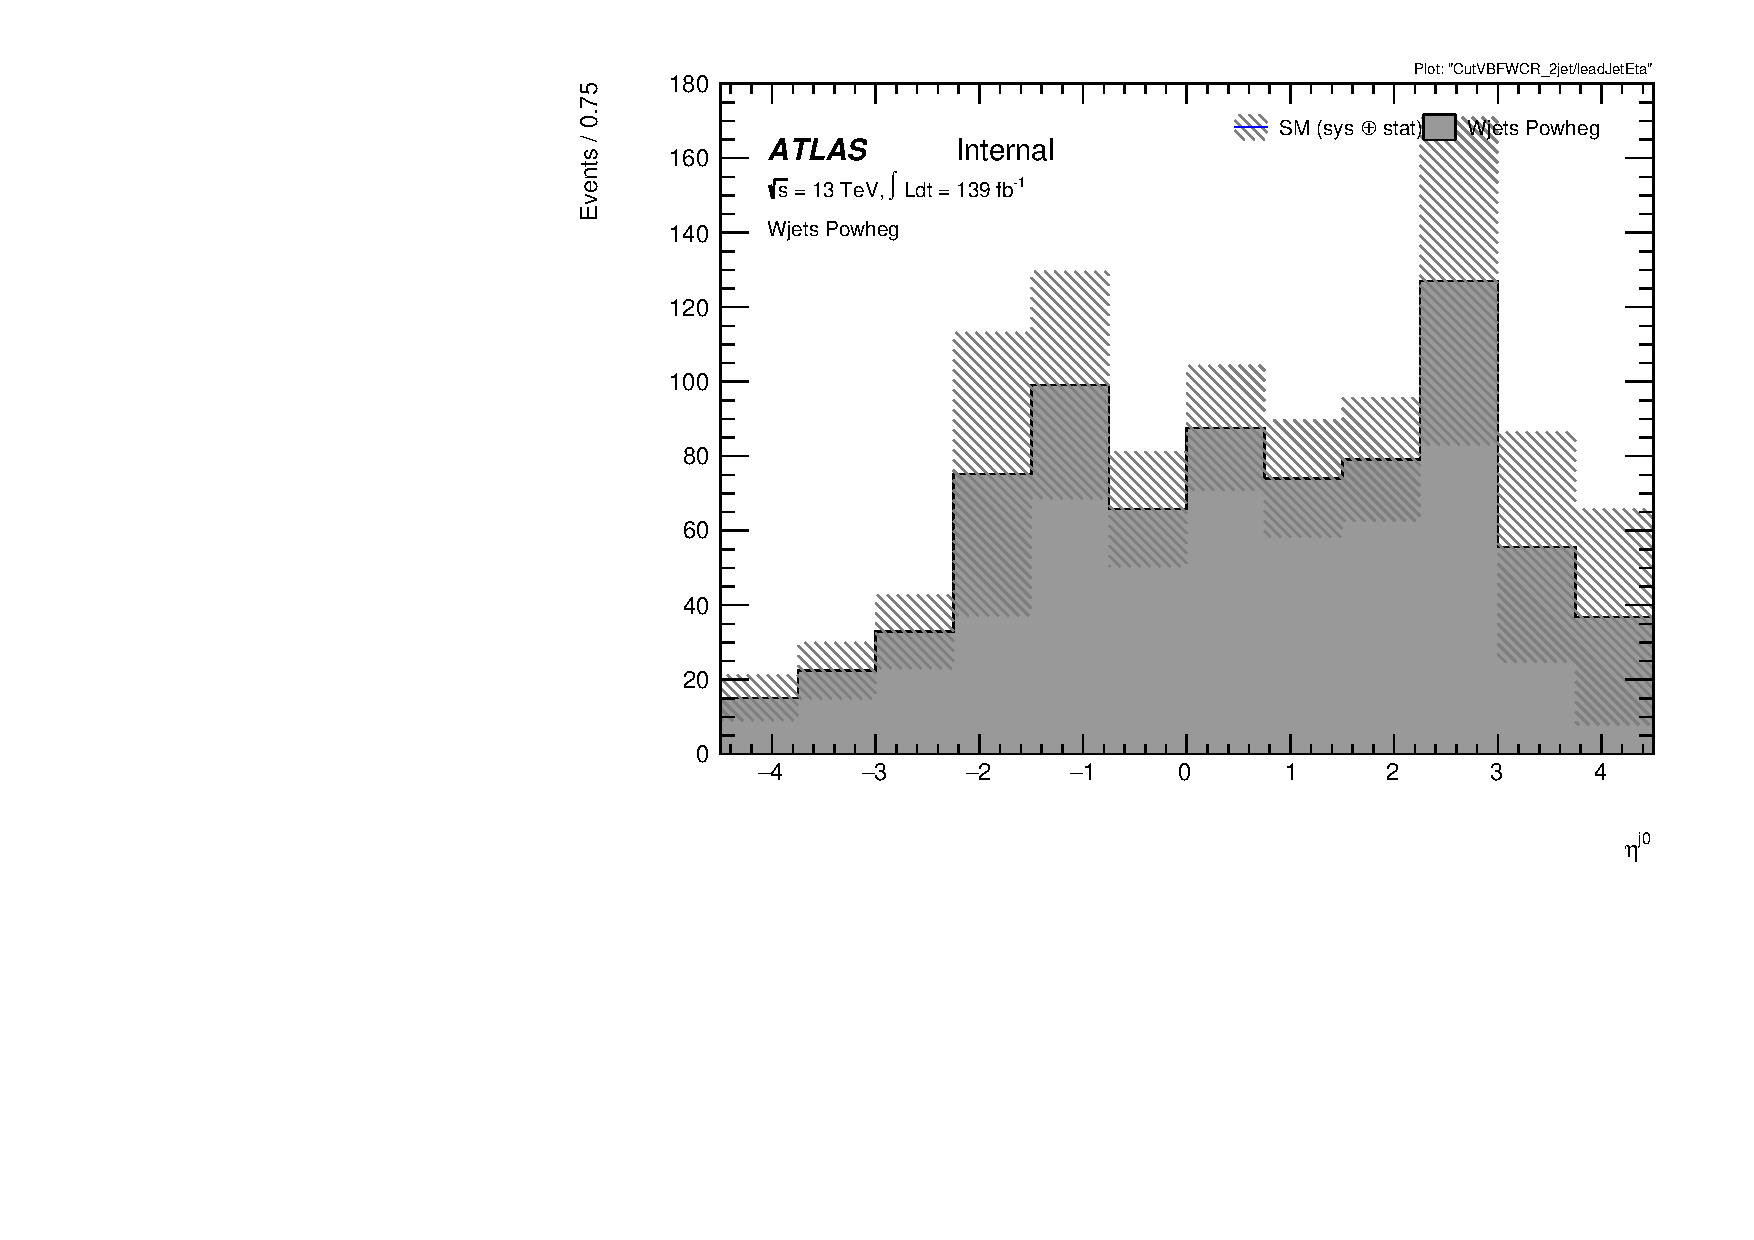
\includegraphics[width=0.23\textwidth]{FakeClosure/run2-emme-CutVBFWCR_2jet-leadJetEta-lin.pdf}
  }\hfill
  \subfloat[$\eta^{j1}$]{
      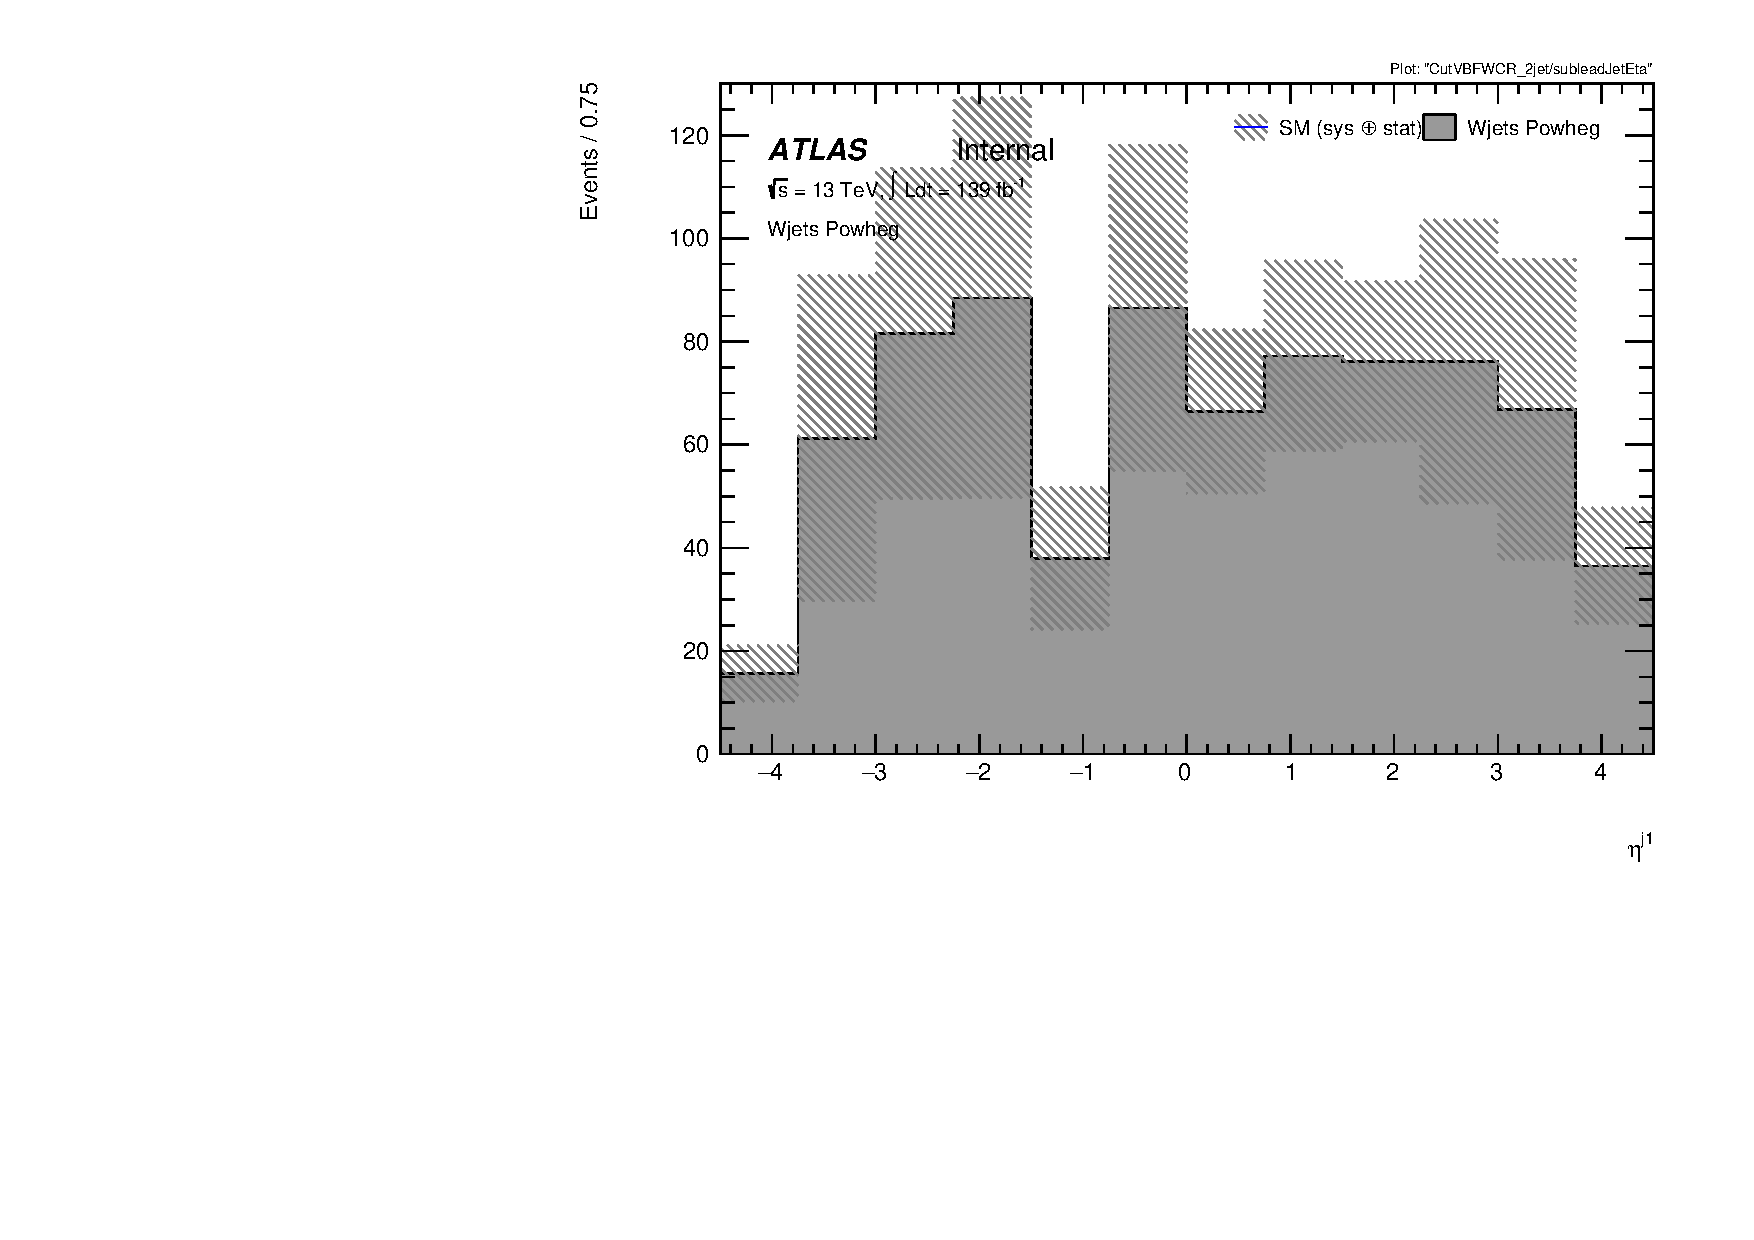
\includegraphics[width=0.23\textwidth]{FakeClosure/run2-emme-CutVBFWCR_2jet-subleadJetEta-lin.pdf}
  }%\hfill
{\caption{Distributions after preselection, FF and 2-jets cuts for $W+$jets MC samples in the $W+$jets control region (id-anti-id).
\label{fig:WCR2jet}}}
\end{figure}

\begin{figure}[!h]
\centering
  \subfloat[$m_{jj}$]{
      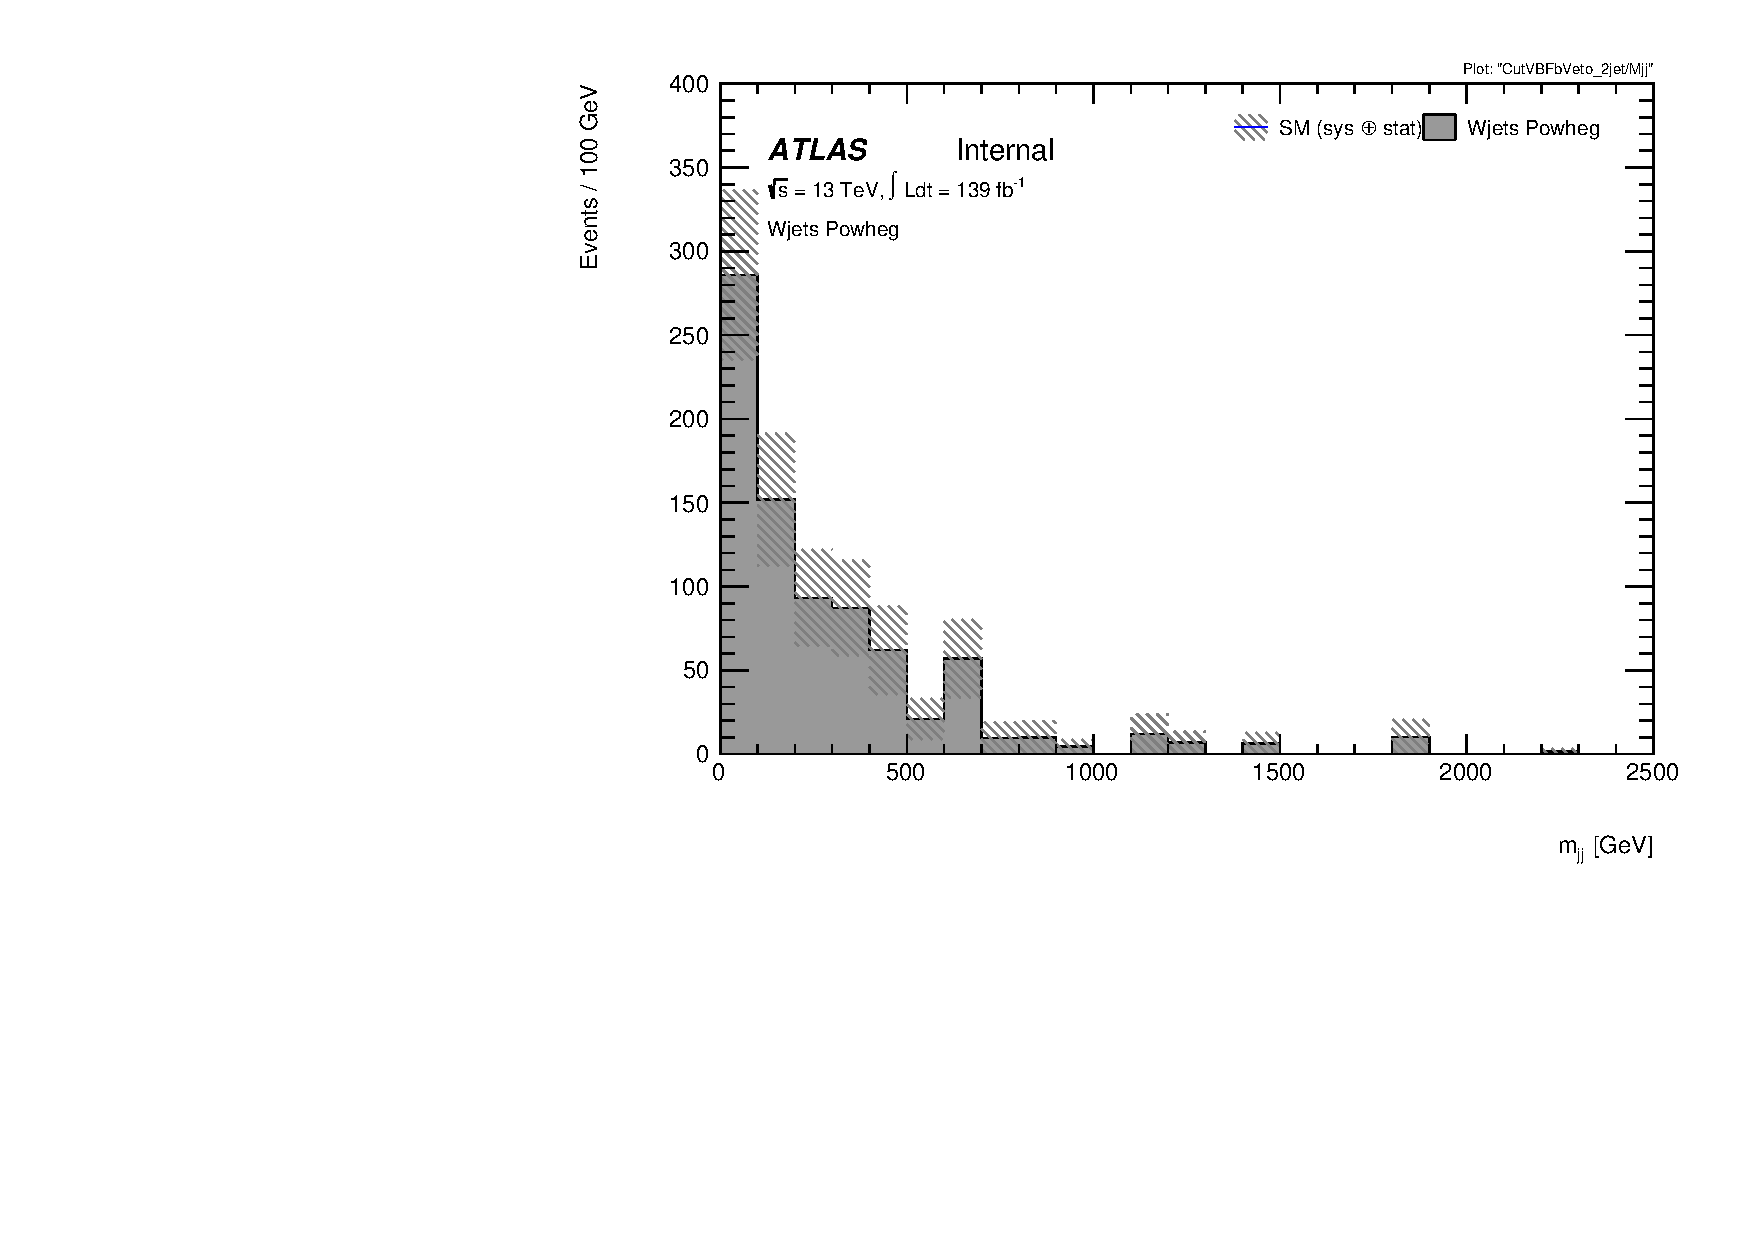
\includegraphics[width=0.3\textwidth]{FakeClosure/run2-emme-CutVBFbVeto_2jet-Mjj-lin.pdf}
  }\hfill
  \subfloat[$p^H_{T}$]{
      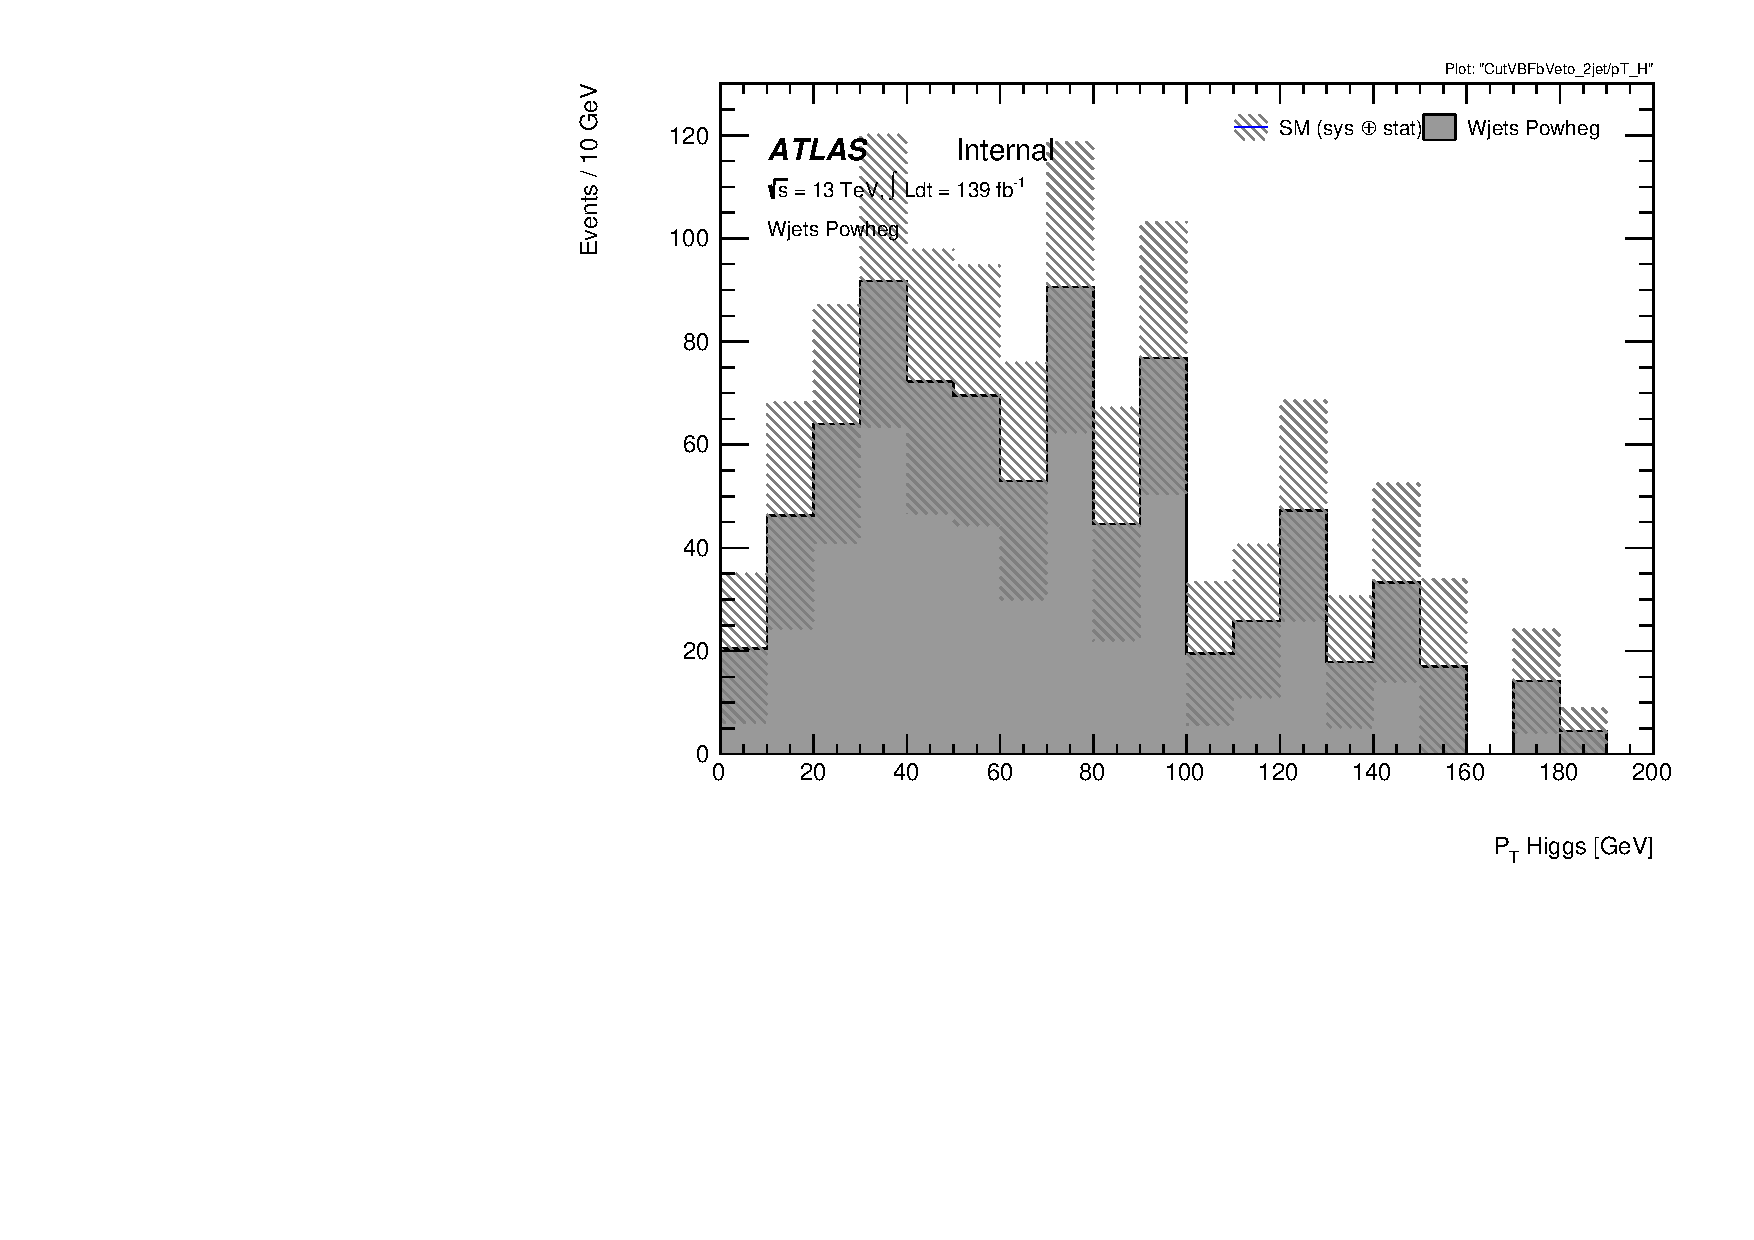
\includegraphics[width=0.3\textwidth]{FakeClosure/run2-emme-CutVBFbVeto_2jet-pT_H-lin.pdf}
  }\hfill
  \subfloat[$p_T^{l0}$]{
      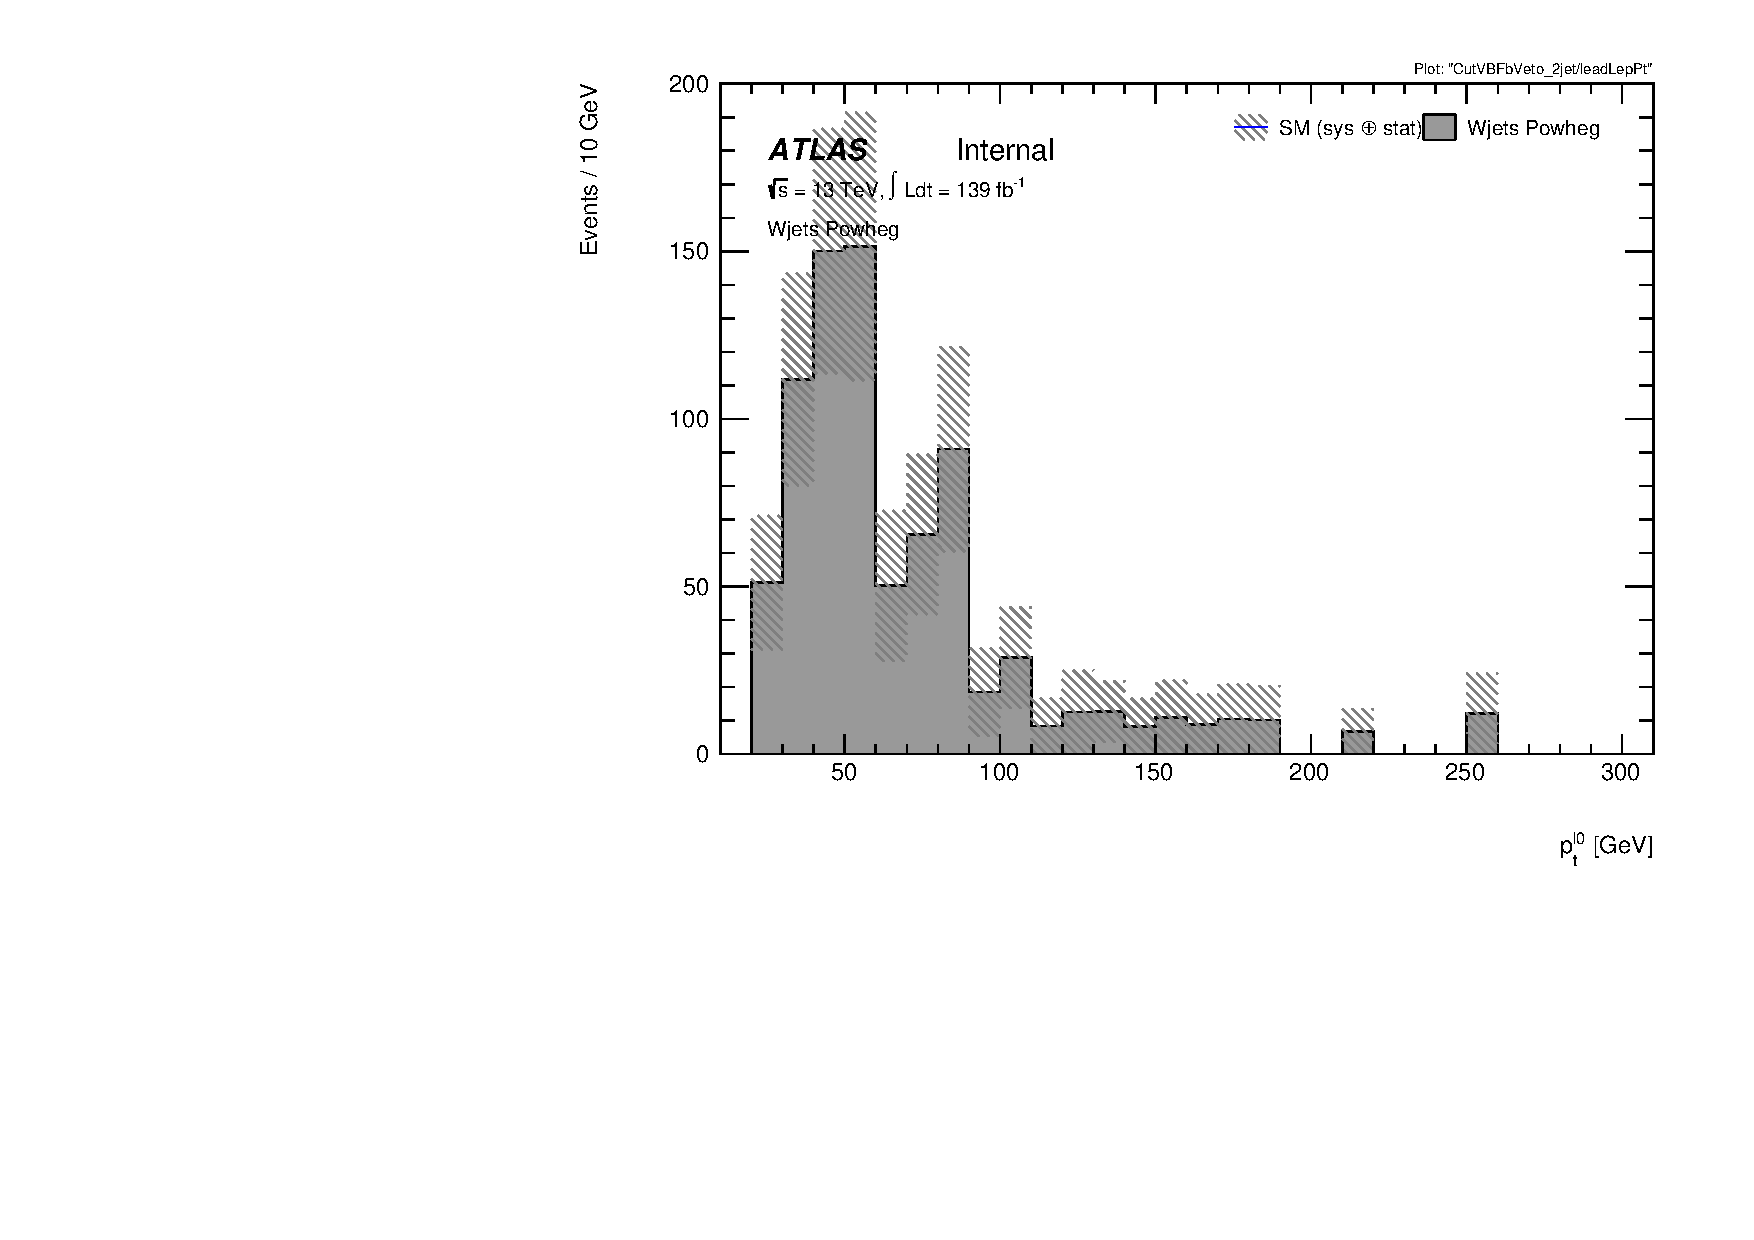
\includegraphics[width=0.3\textwidth]{FakeClosure/run2-emme-CutVBFbVeto_2jet-leadLepPt-lin.pdf}
  }\hfill
  \subfloat[$p_T^{l1}$]{
      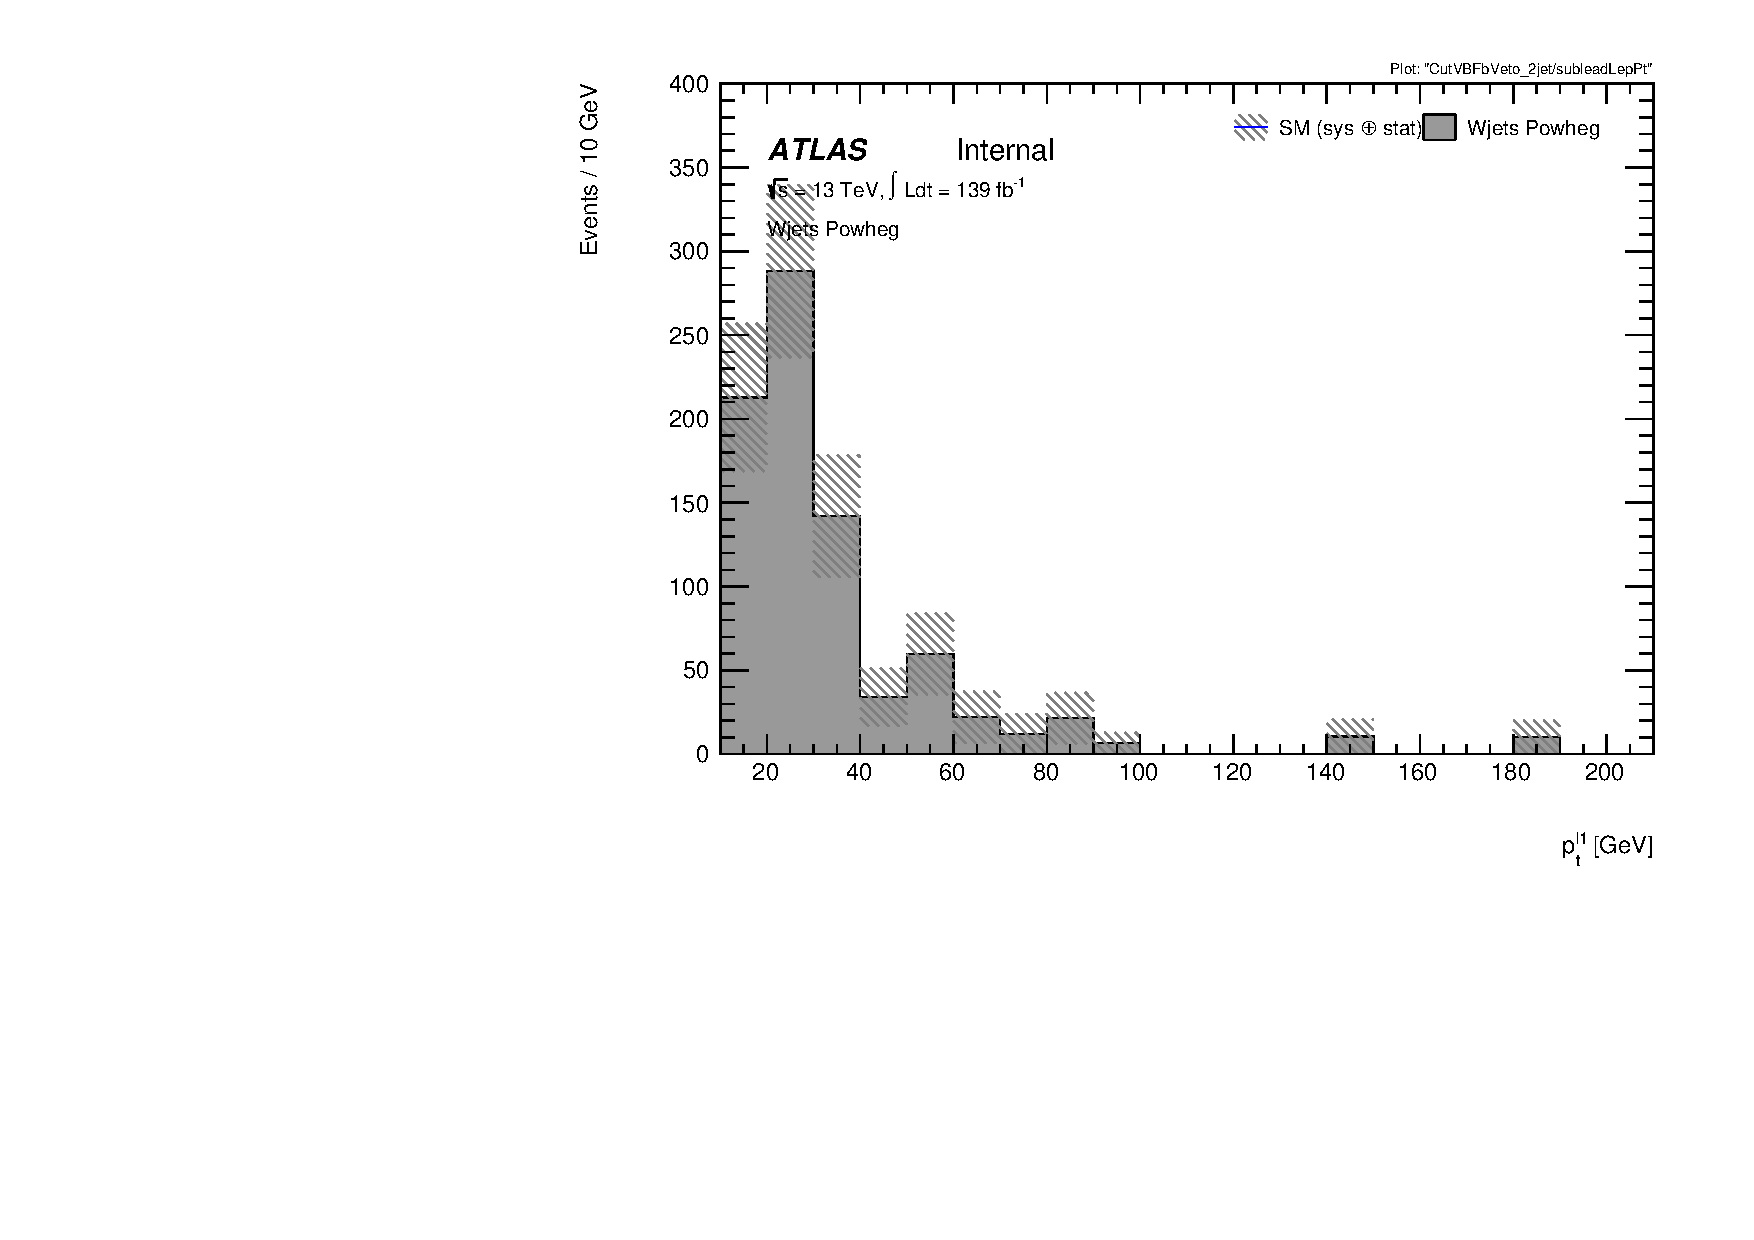
\includegraphics[width=0.3\textwidth]{FakeClosure/run2-emme-CutVBFbVeto_2jet-subleadLepPt-lin.pdf}
  }\hfill
  \subfloat[$p_T^{j0}$]{
      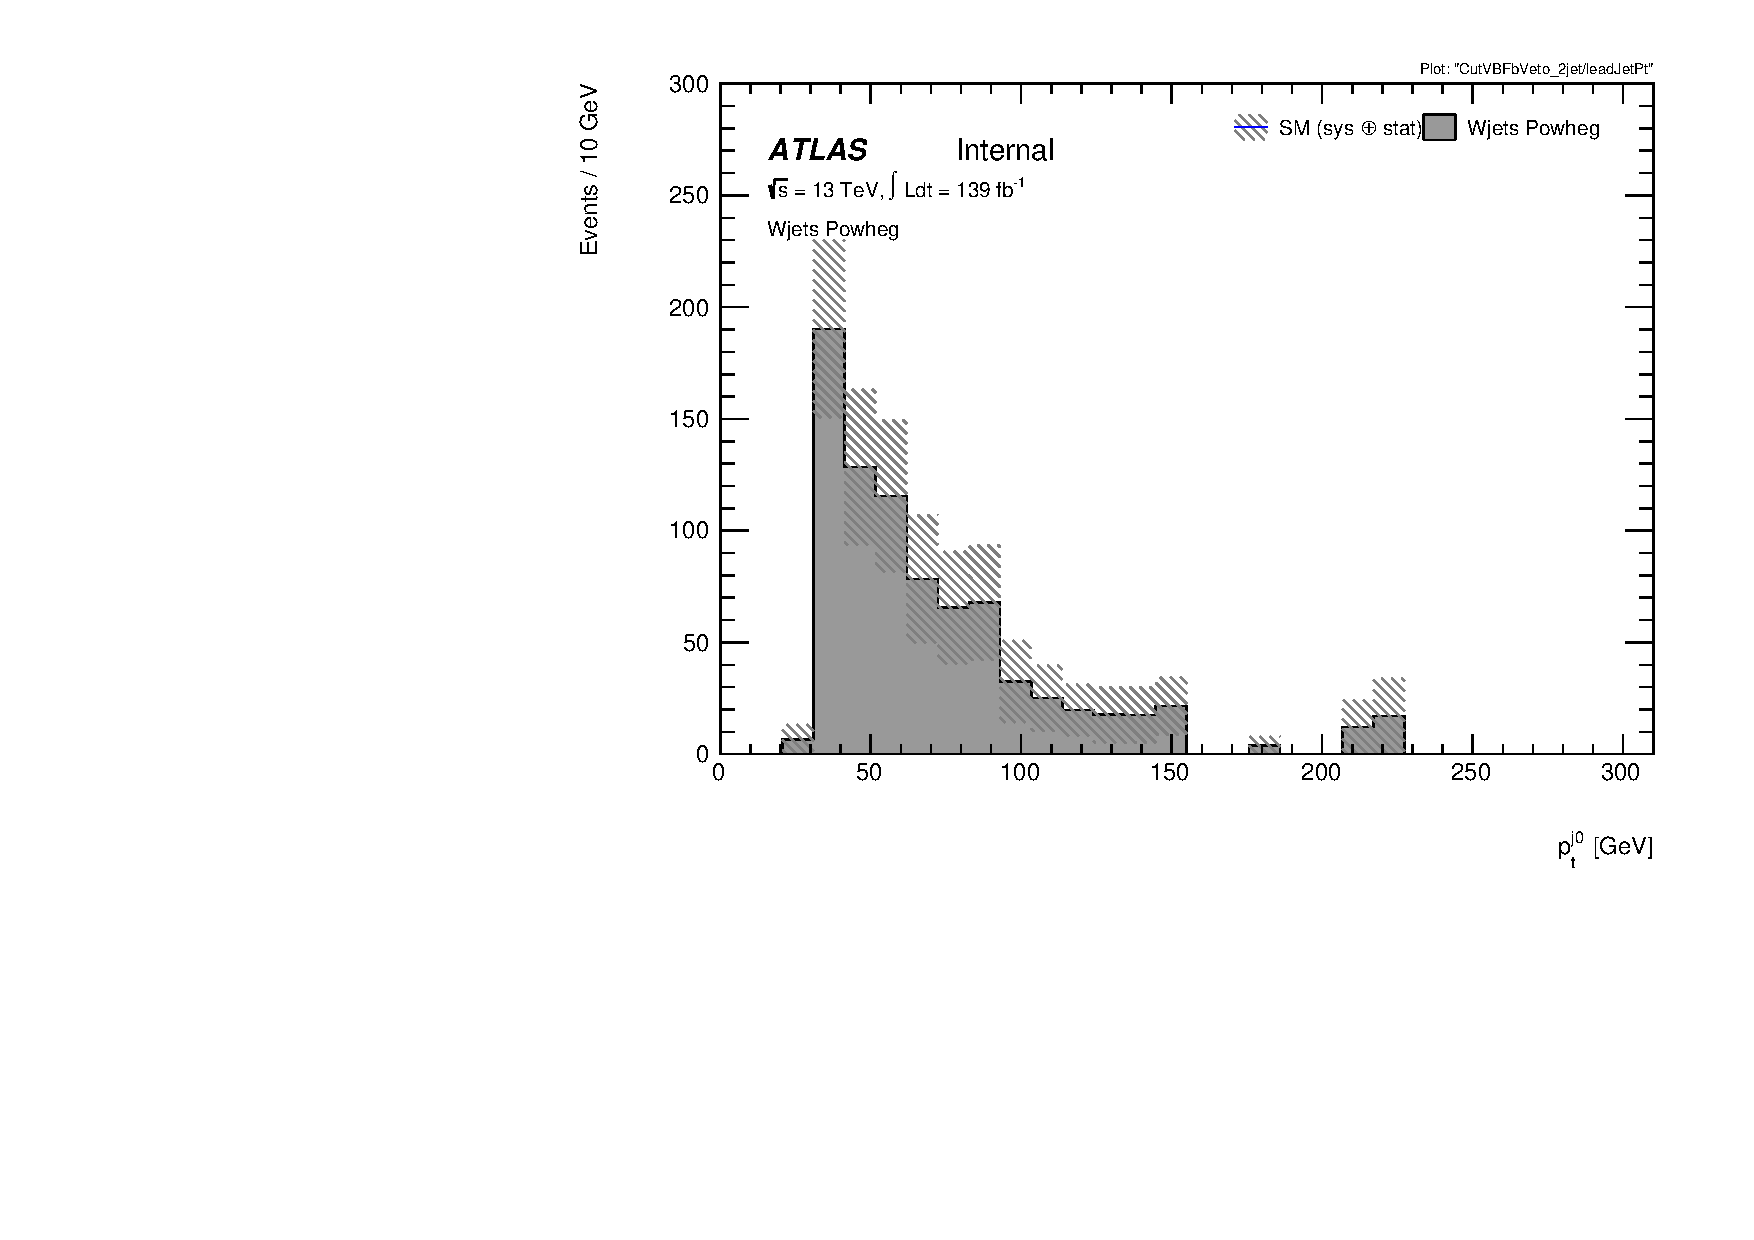
\includegraphics[width=0.3\textwidth]{FakeClosure/run2-emme-CutVBFbVeto_2jet-leadJetPt-lin.pdf}
  }\hfill
  \subfloat[$p_T^{j1}$]{
      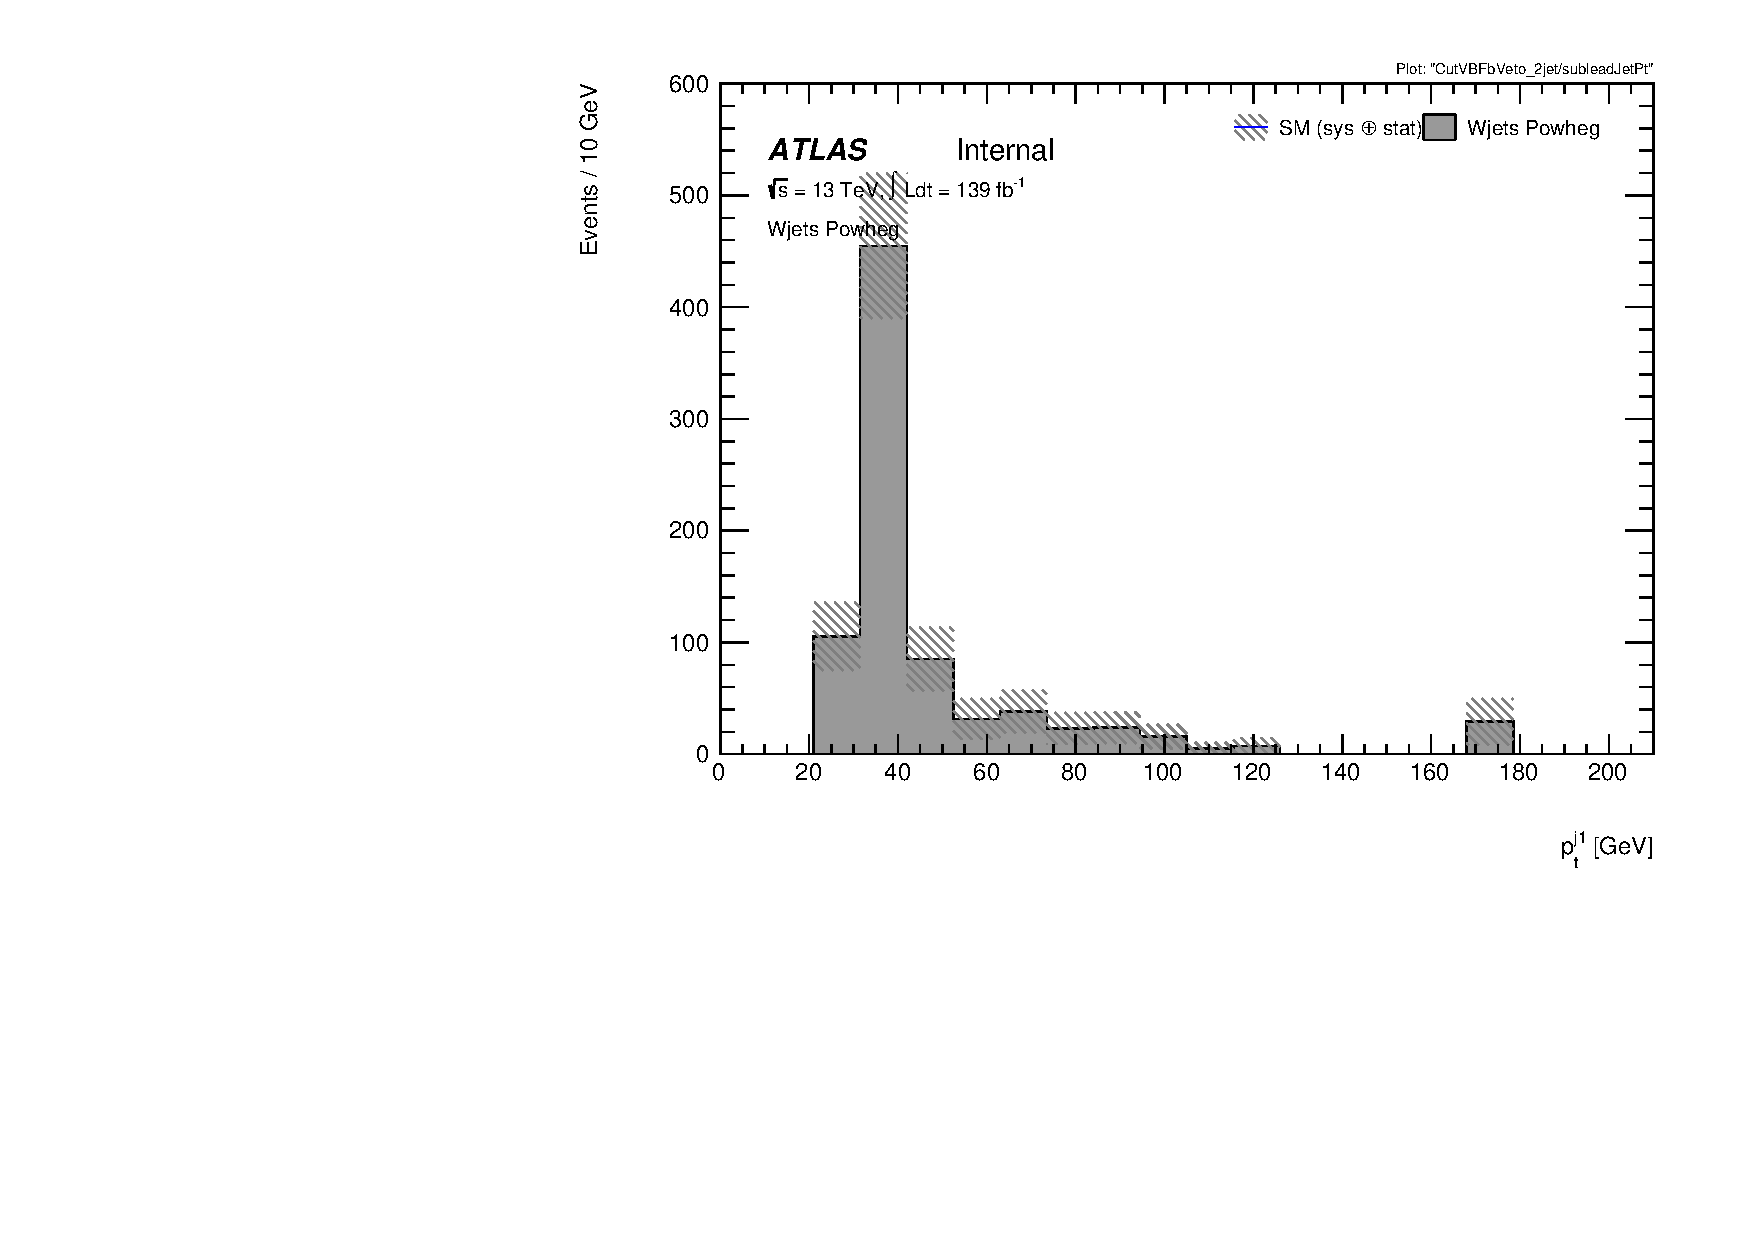
\includegraphics[width=0.3\textwidth]{FakeClosure/run2-emme-CutVBFbVeto_2jet-subleadJetPt-lin.pdf}
  }\hfill
  \subfloat[$\eta^{l0}$]{
      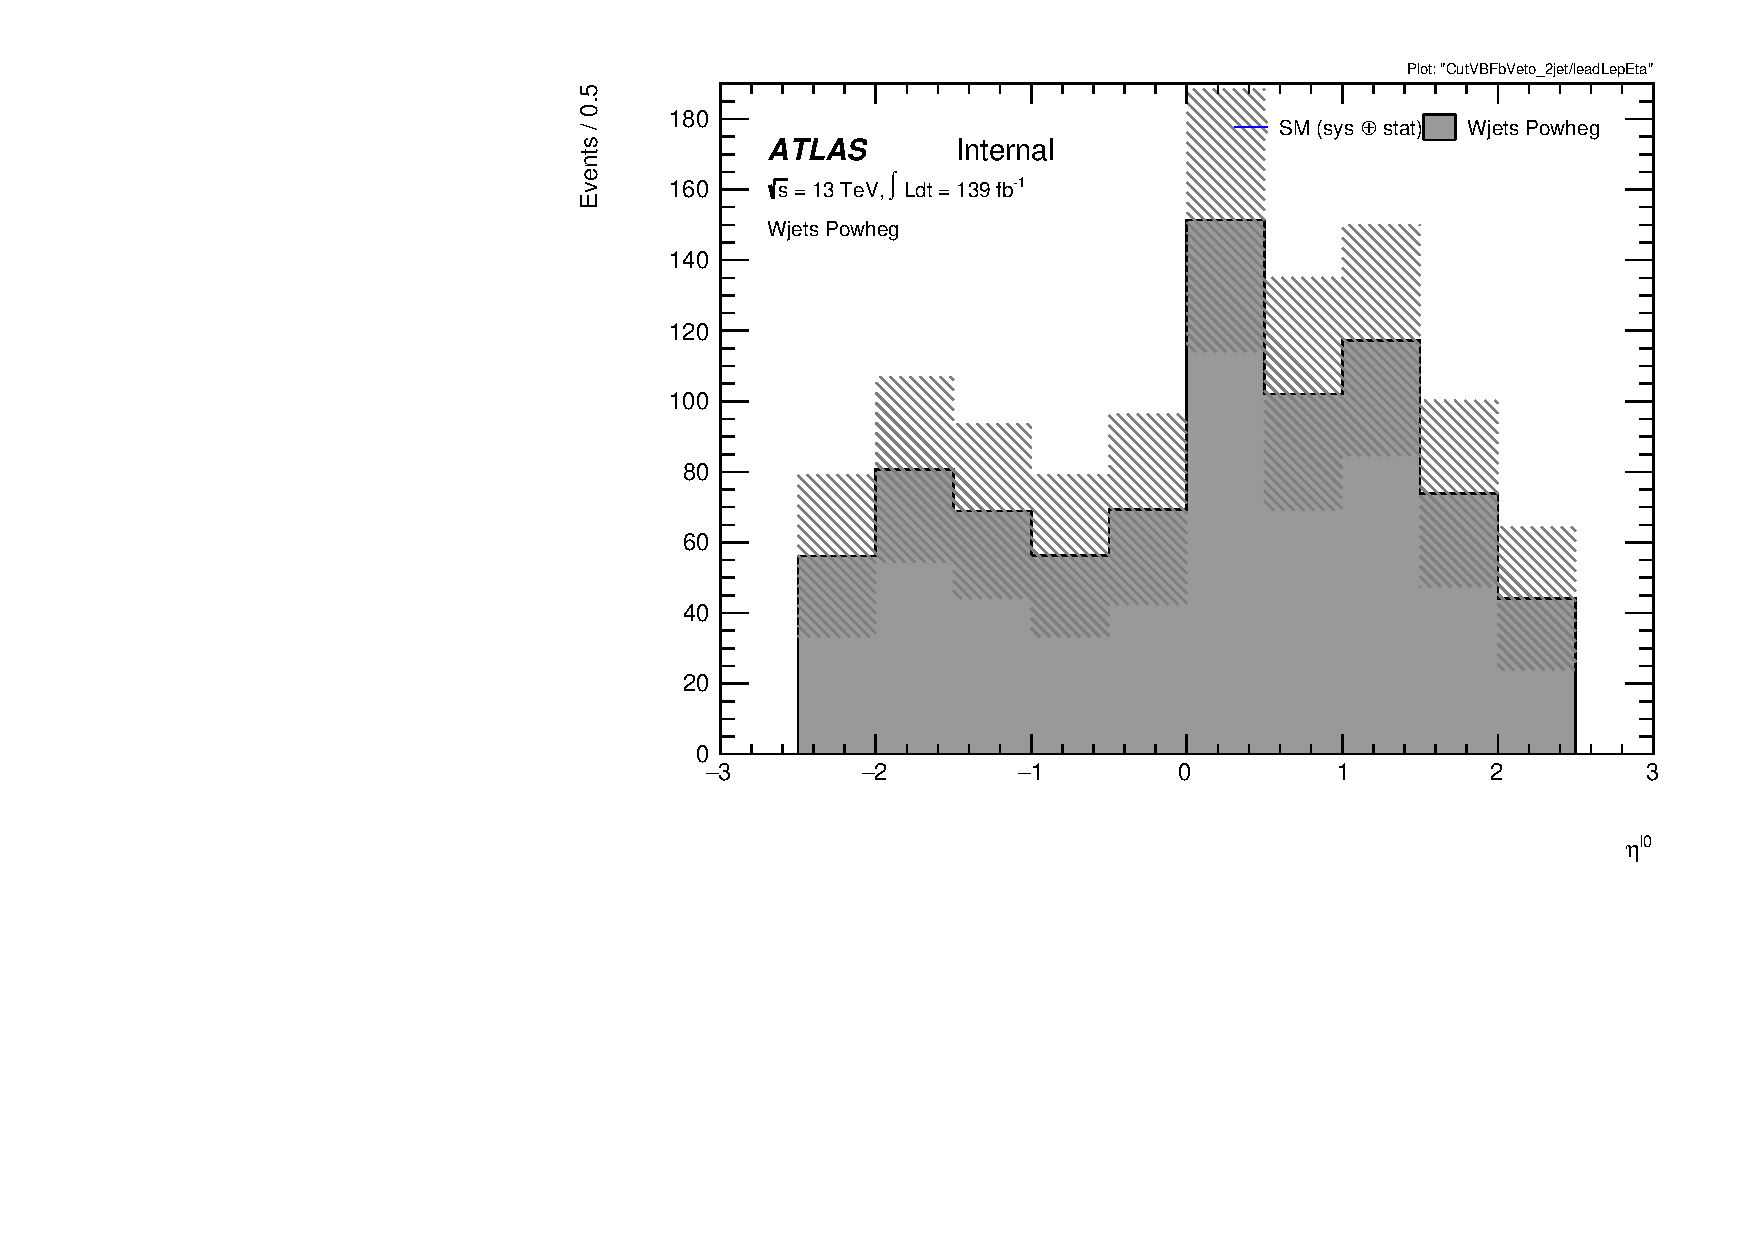
\includegraphics[width=0.23\textwidth]{FakeClosure/run2-emme-CutVBFbVeto_2jet-leadLepEta-lin.pdf}
  }\hfill
  \subfloat[$\eta^{l1}$]{
      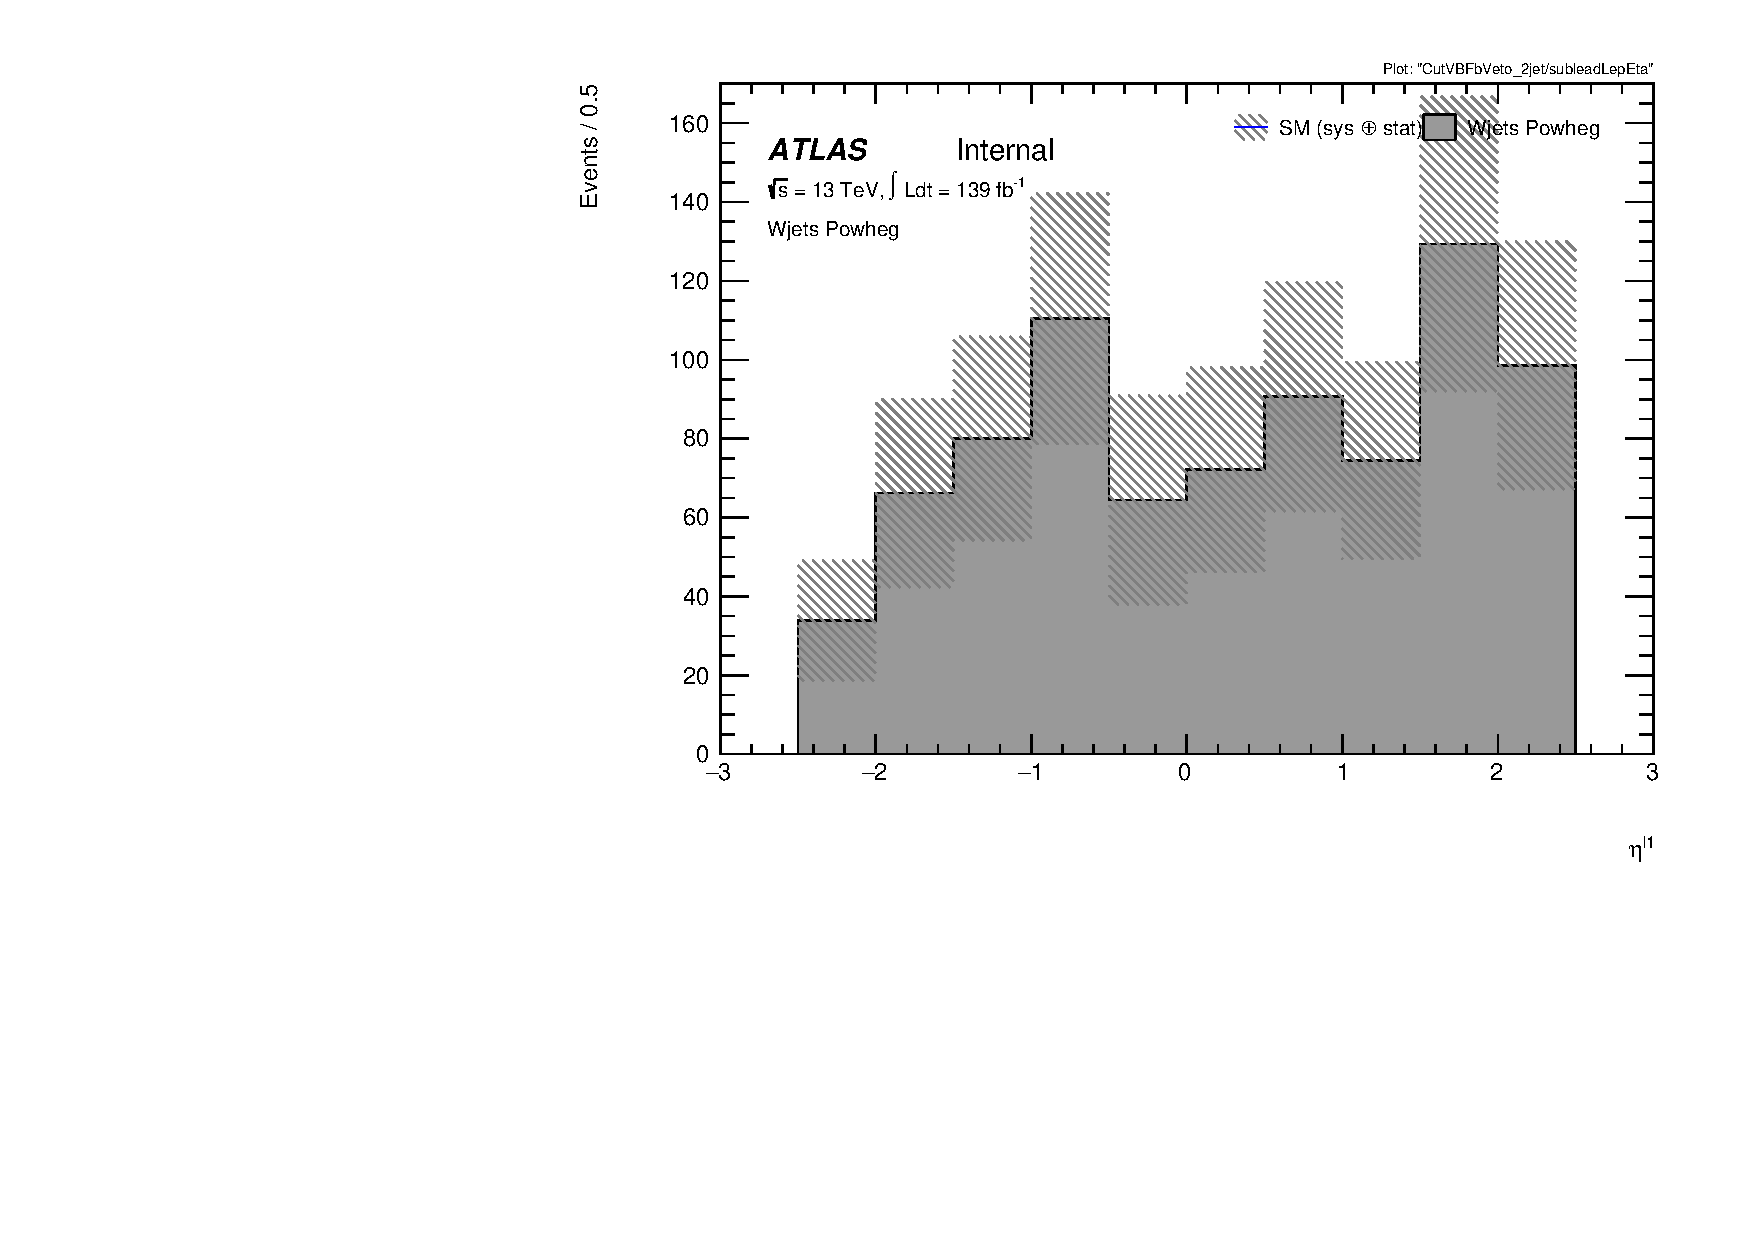
\includegraphics[width=0.23\textwidth]{FakeClosure/run2-emme-CutVBFbVeto_2jet-subleadLepEta-lin.pdf}
  }\hfill
  \subfloat[$\eta^{j0}$]{
      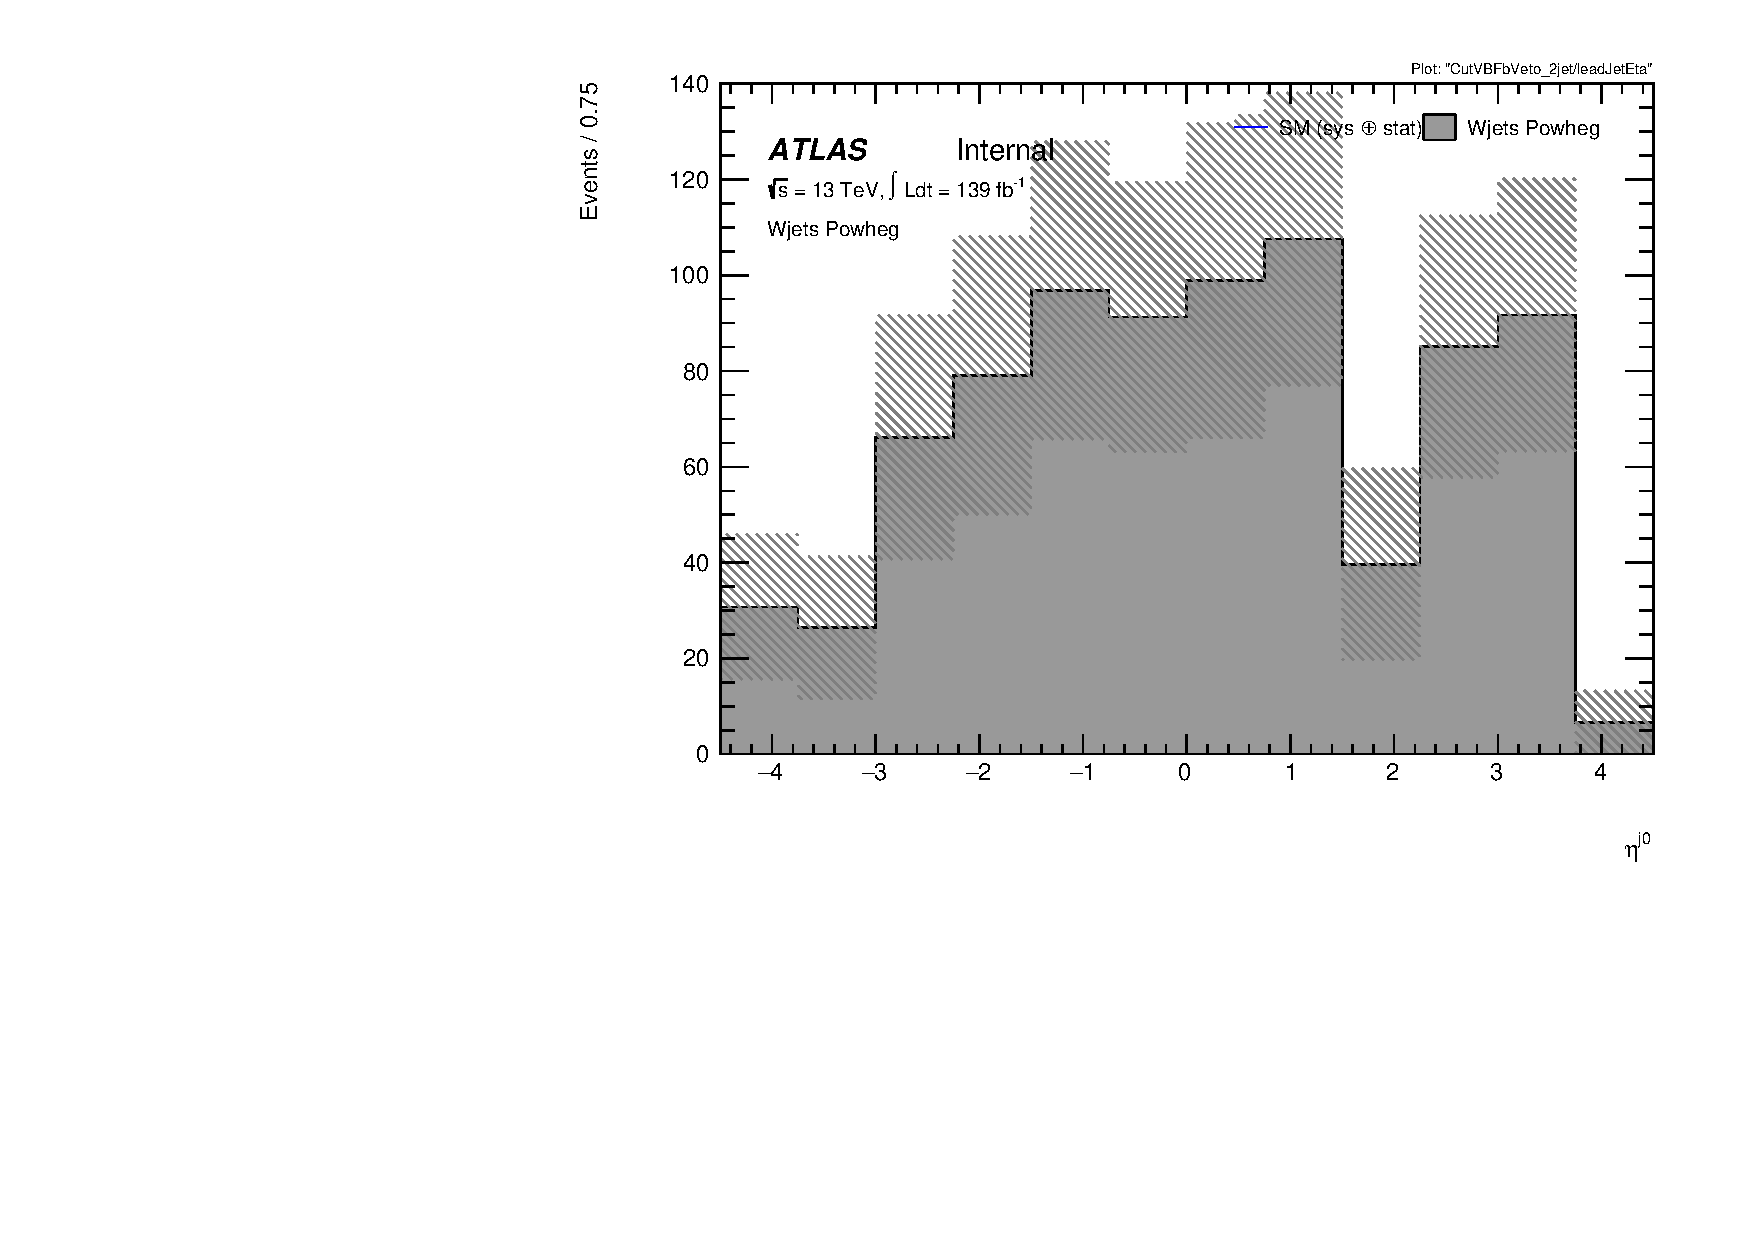
\includegraphics[width=0.23\textwidth]{FakeClosure/run2-emme-CutVBFbVeto_2jet-leadJetEta-lin.pdf}
  }\hfill
  \subfloat[$\eta^{j1}$]{
      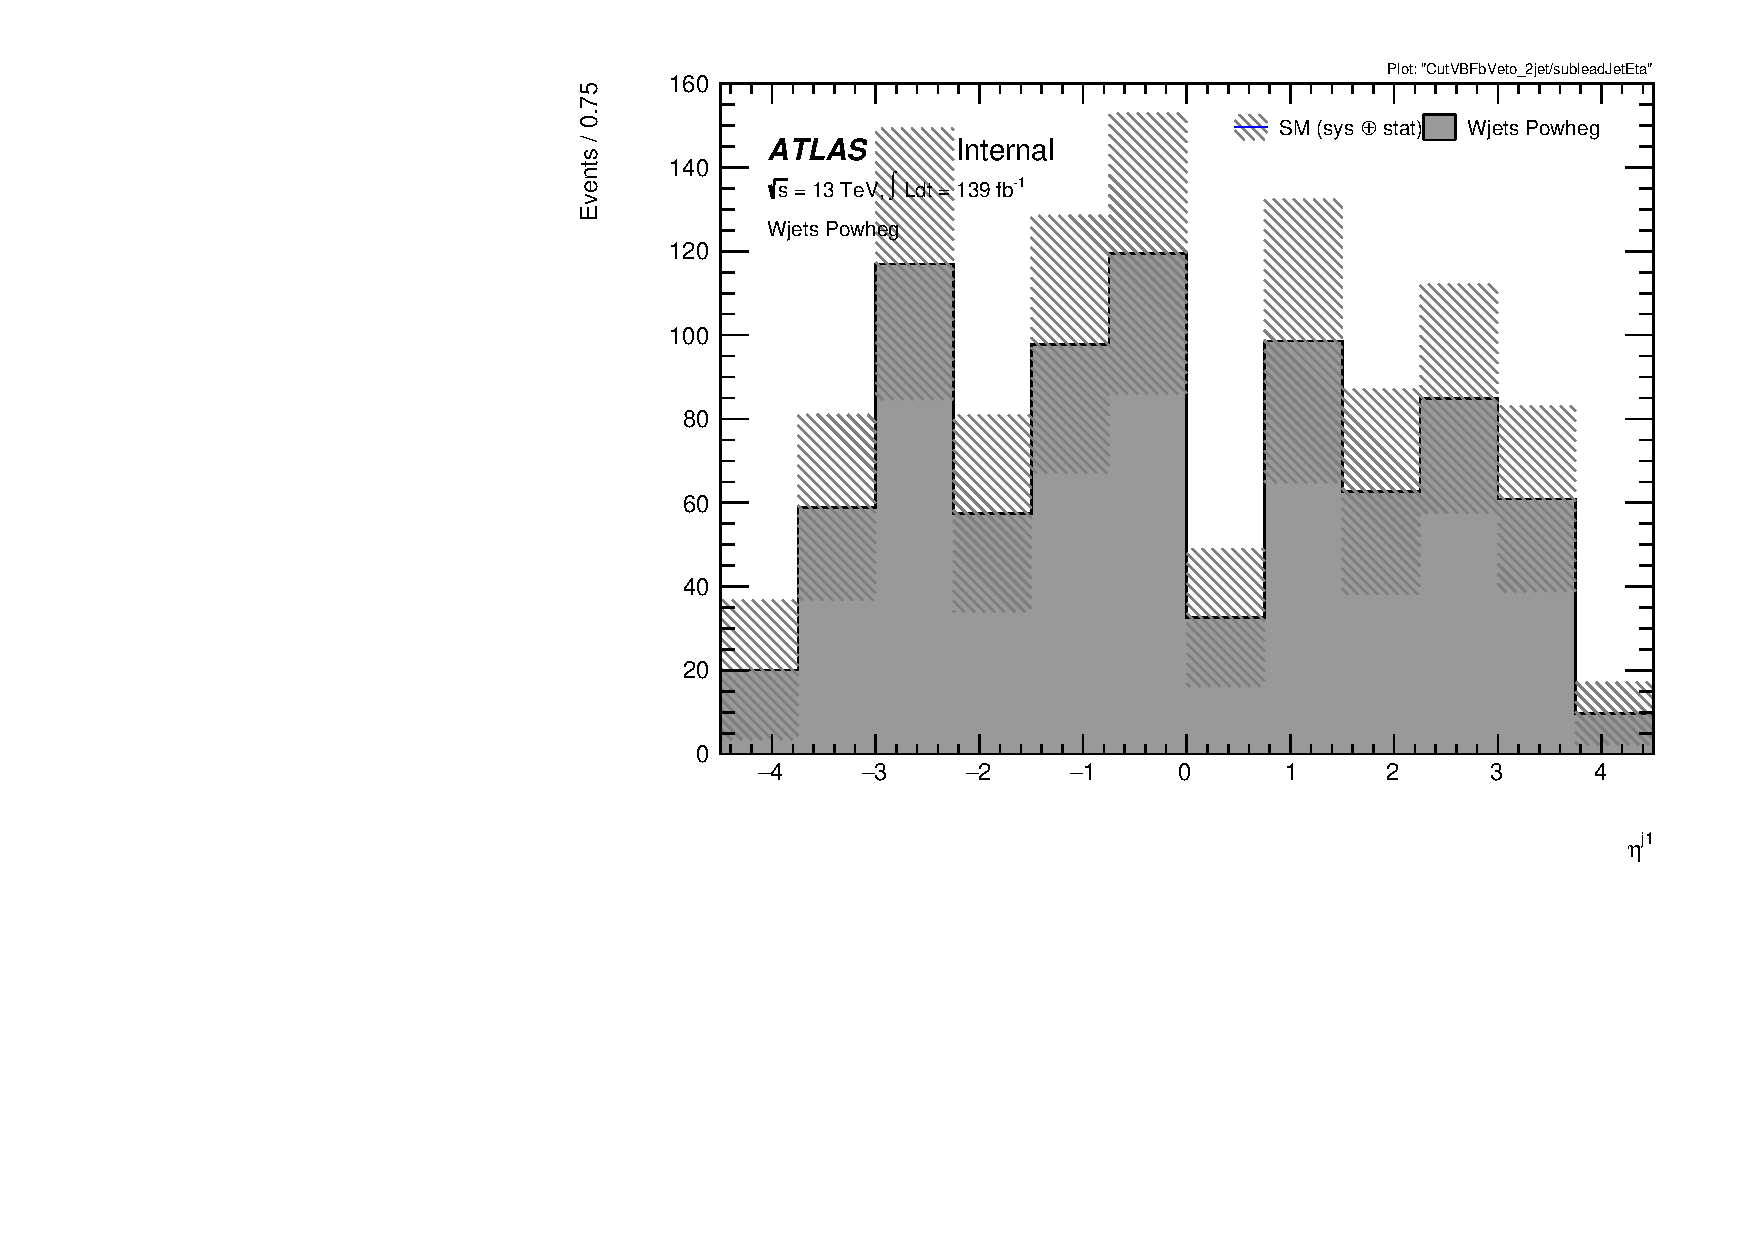
\includegraphics[width=0.23\textwidth]{FakeClosure/run2-emme-CutVBFbVeto_2jet-subleadJetEta-lin.pdf}
  }%\hfill
{\caption{Distributions after preselection, 2-jets and b-veto cuts for $W+$jets MC samples in the signal region (id-id).
\label{fig:SR2jet}}}
\end{figure}


\begin{figure}[!h]
\centering
  \subfloat[$m_{jj}$]{
      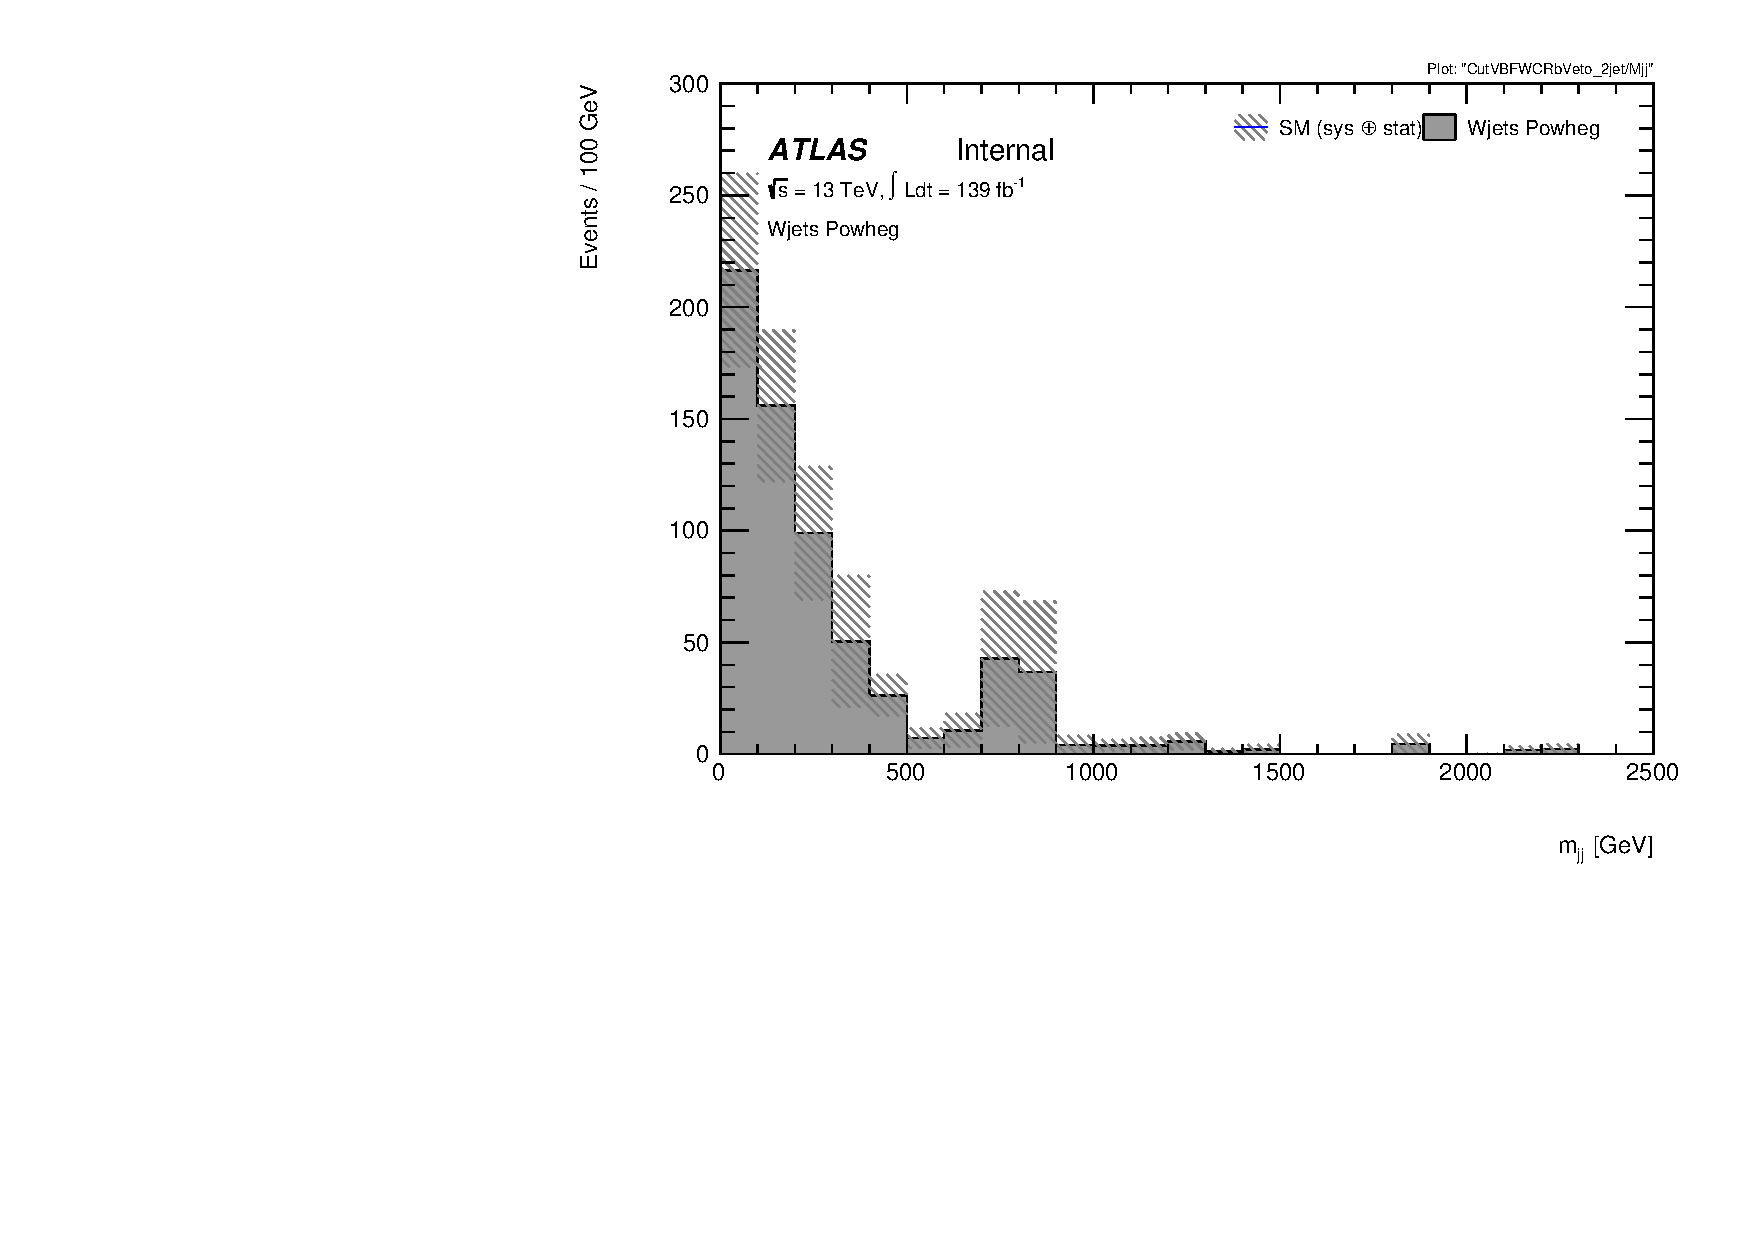
\includegraphics[width=0.3\textwidth]{FakeClosure/run2-emme-CutVBFWCRbVeto_2jet-Mjj-lin.pdf}
  }\hfill
  \subfloat[$p^H_{T}$]{
      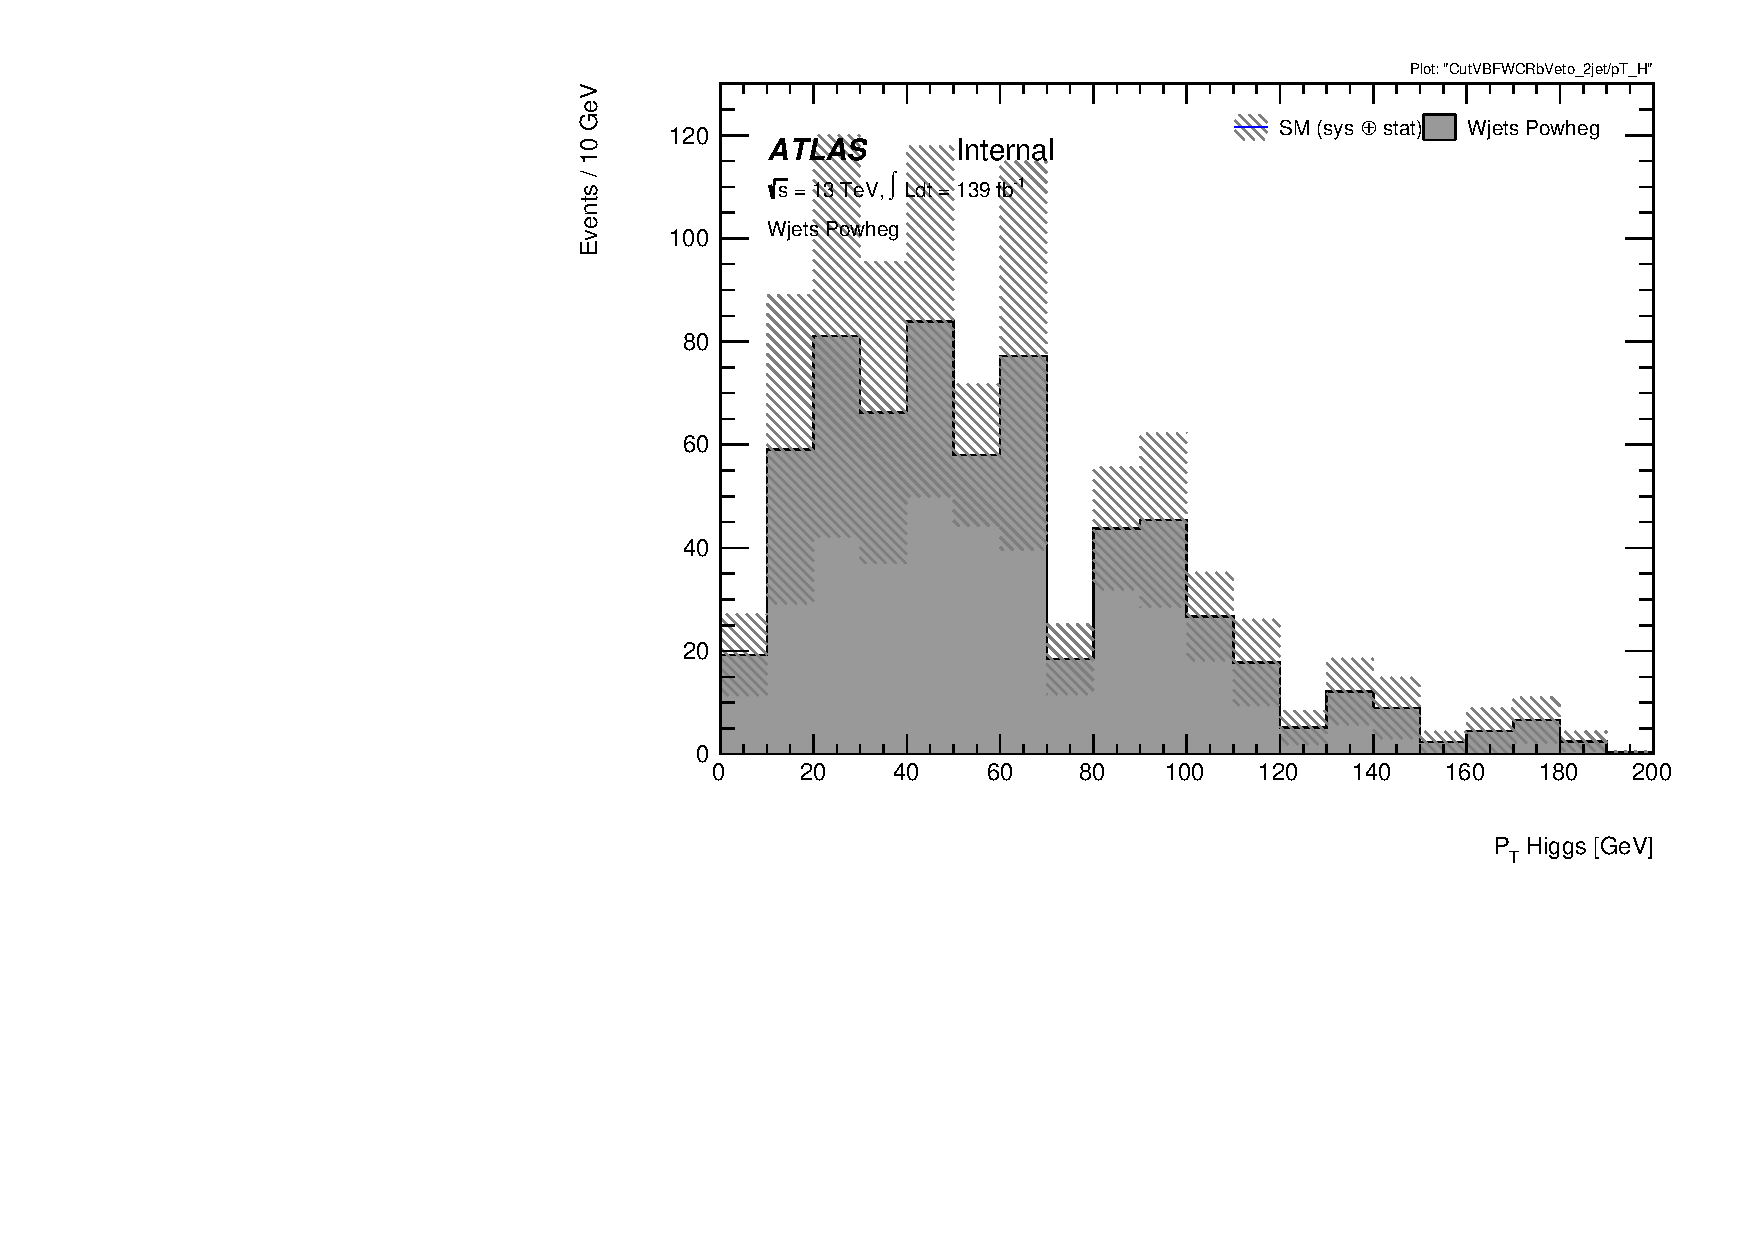
\includegraphics[width=0.3\textwidth]{FakeClosure/run2-emme-CutVBFWCRbVeto_2jet-pT_H-lin.pdf}
  }\hfill
  \subfloat[$p_T^{l0}$]{
      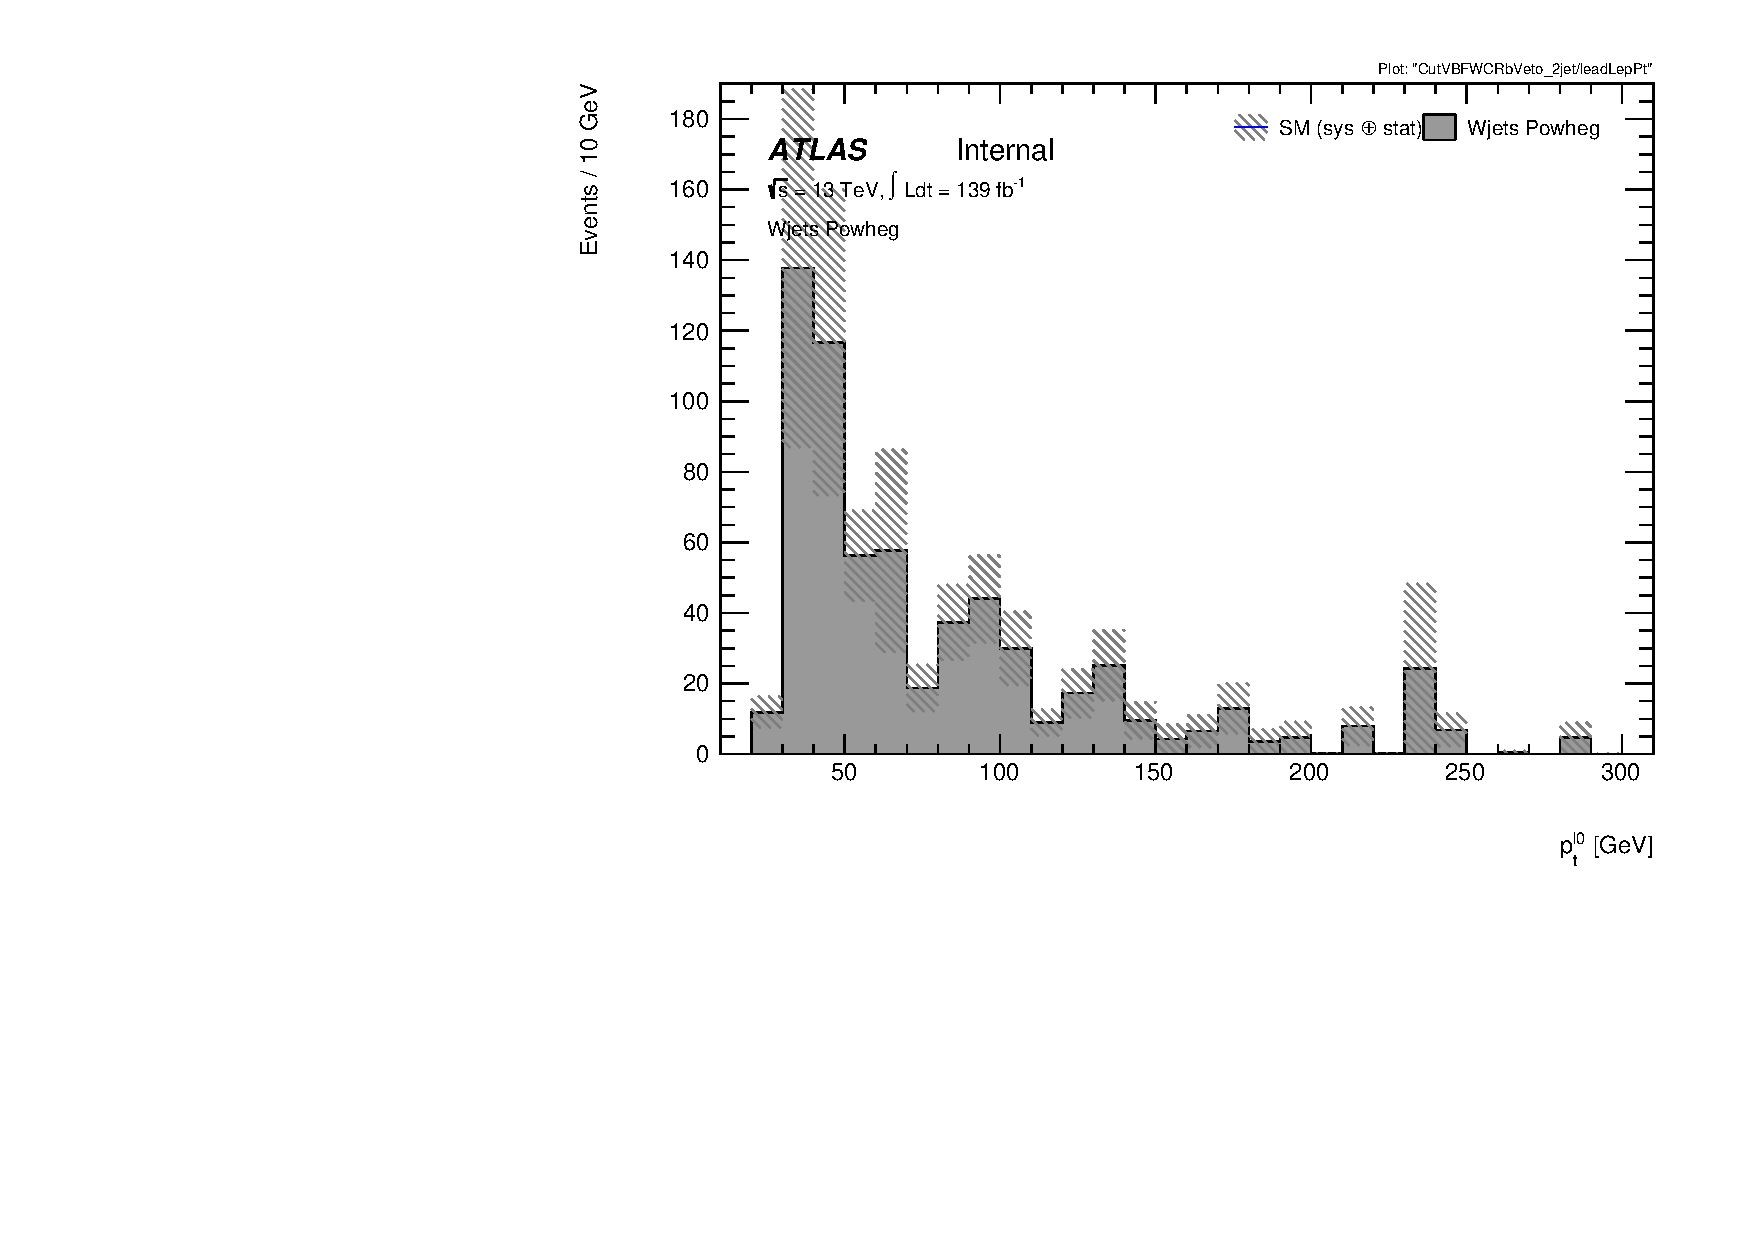
\includegraphics[width=0.3\textwidth]{FakeClosure/run2-emme-CutVBFWCRbVeto_2jet-leadLepPt-lin.pdf}
  }\hfill
  \subfloat[$p_T^{l1}$]{
      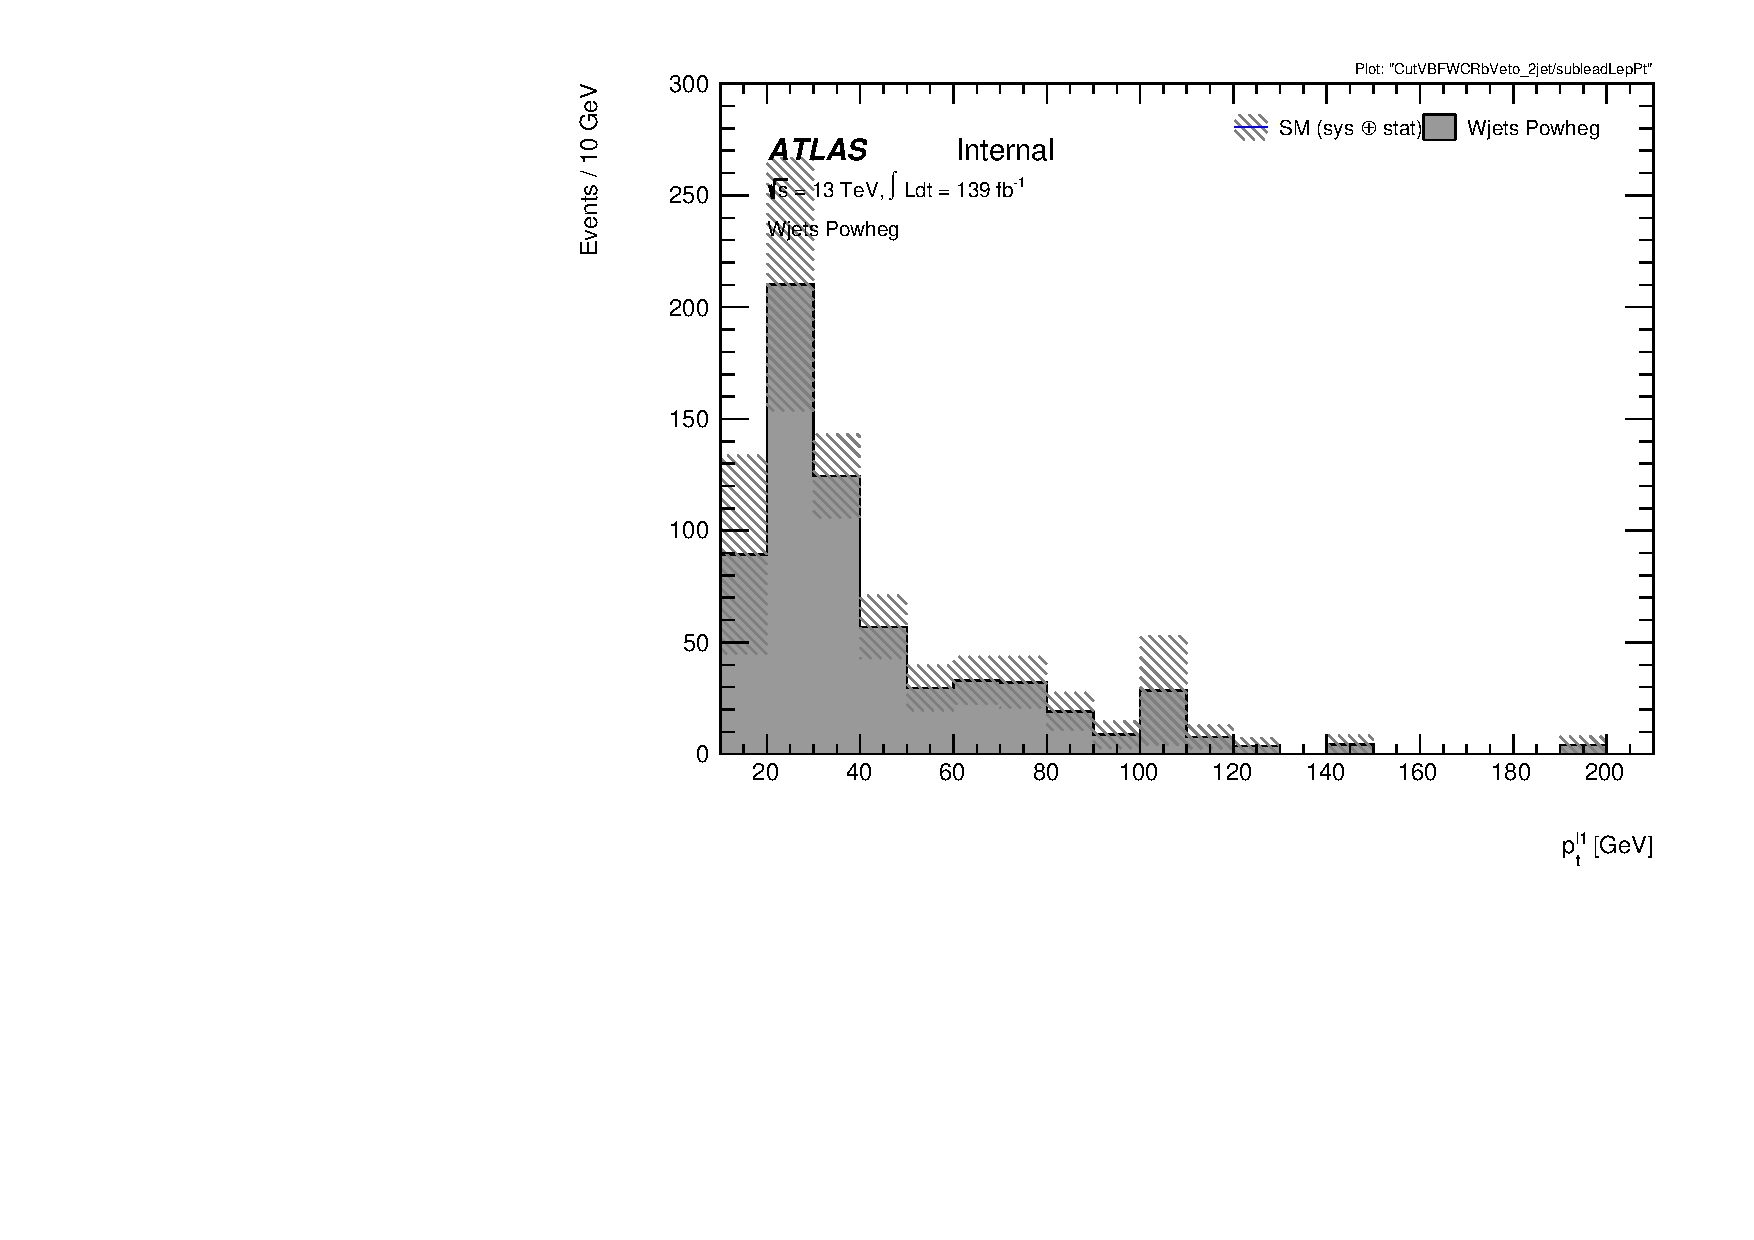
\includegraphics[width=0.3\textwidth]{FakeClosure/run2-emme-CutVBFWCRbVeto_2jet-subleadLepPt-lin.pdf}
  }\hfill
  \subfloat[$p_T^{j0}$]{
      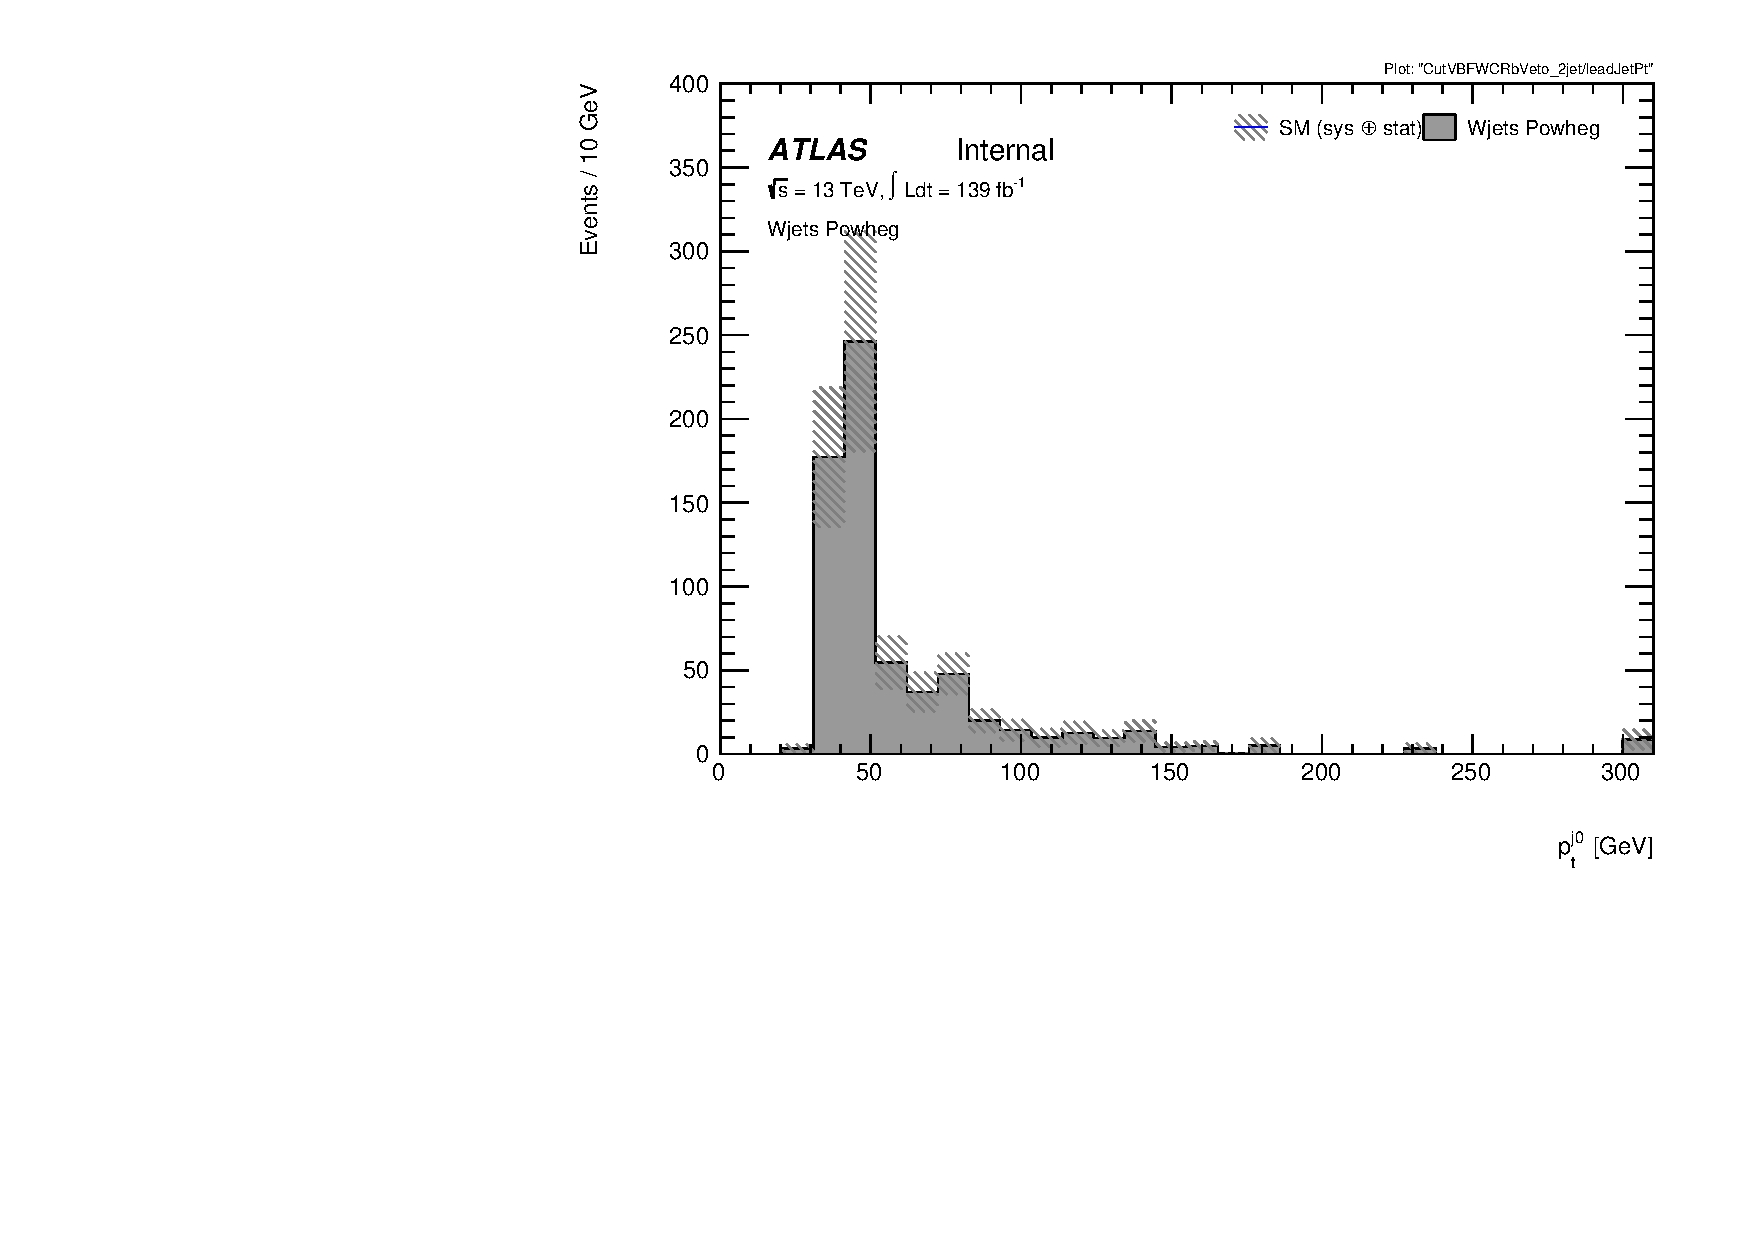
\includegraphics[width=0.3\textwidth]{FakeClosure/run2-emme-CutVBFWCRbVeto_2jet-leadJetPt-lin.pdf}
  }\hfill
  \subfloat[$p_T^{j1}$]{
      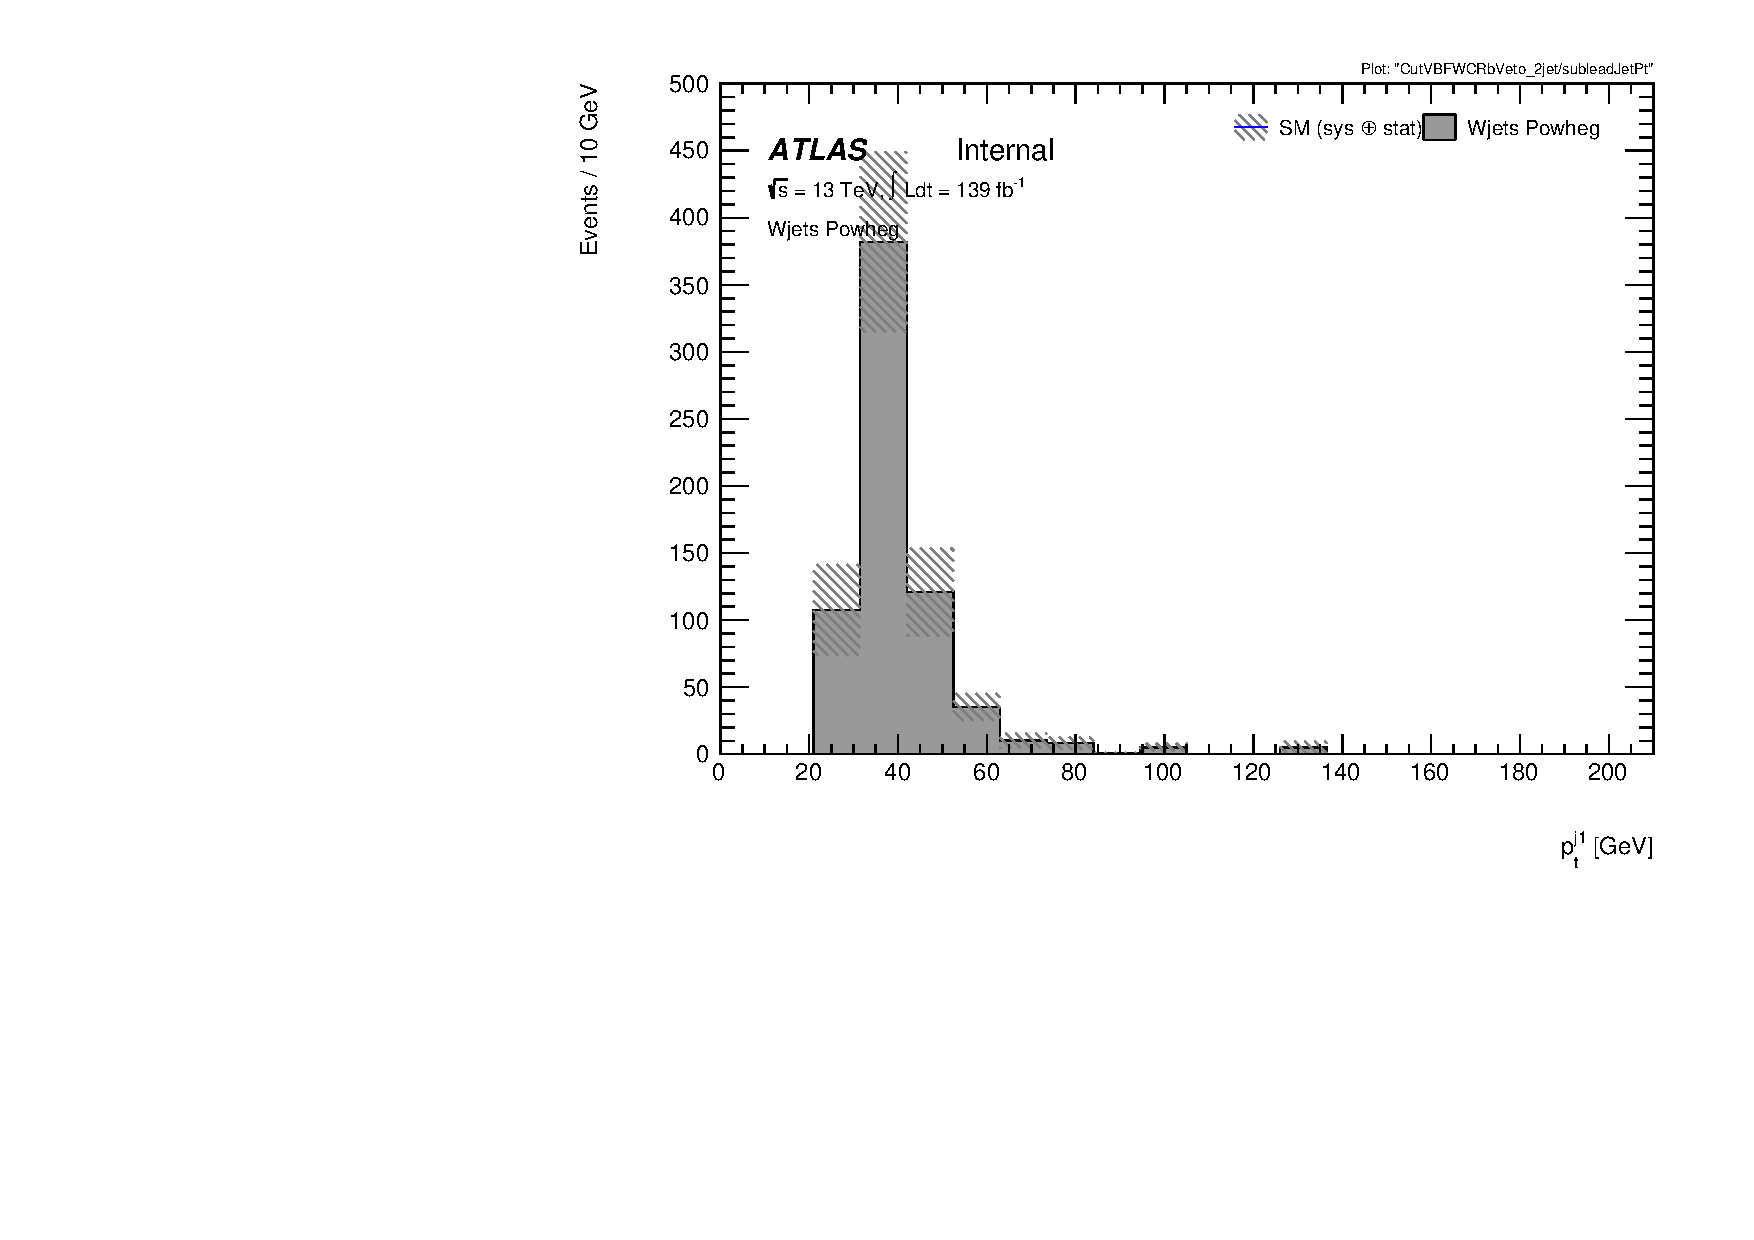
\includegraphics[width=0.3\textwidth]{FakeClosure/run2-emme-CutVBFWCRbVeto_2jet-subleadJetPt-lin.pdf}
  }\hfill
  \subfloat[$\eta^{l0}$]{
      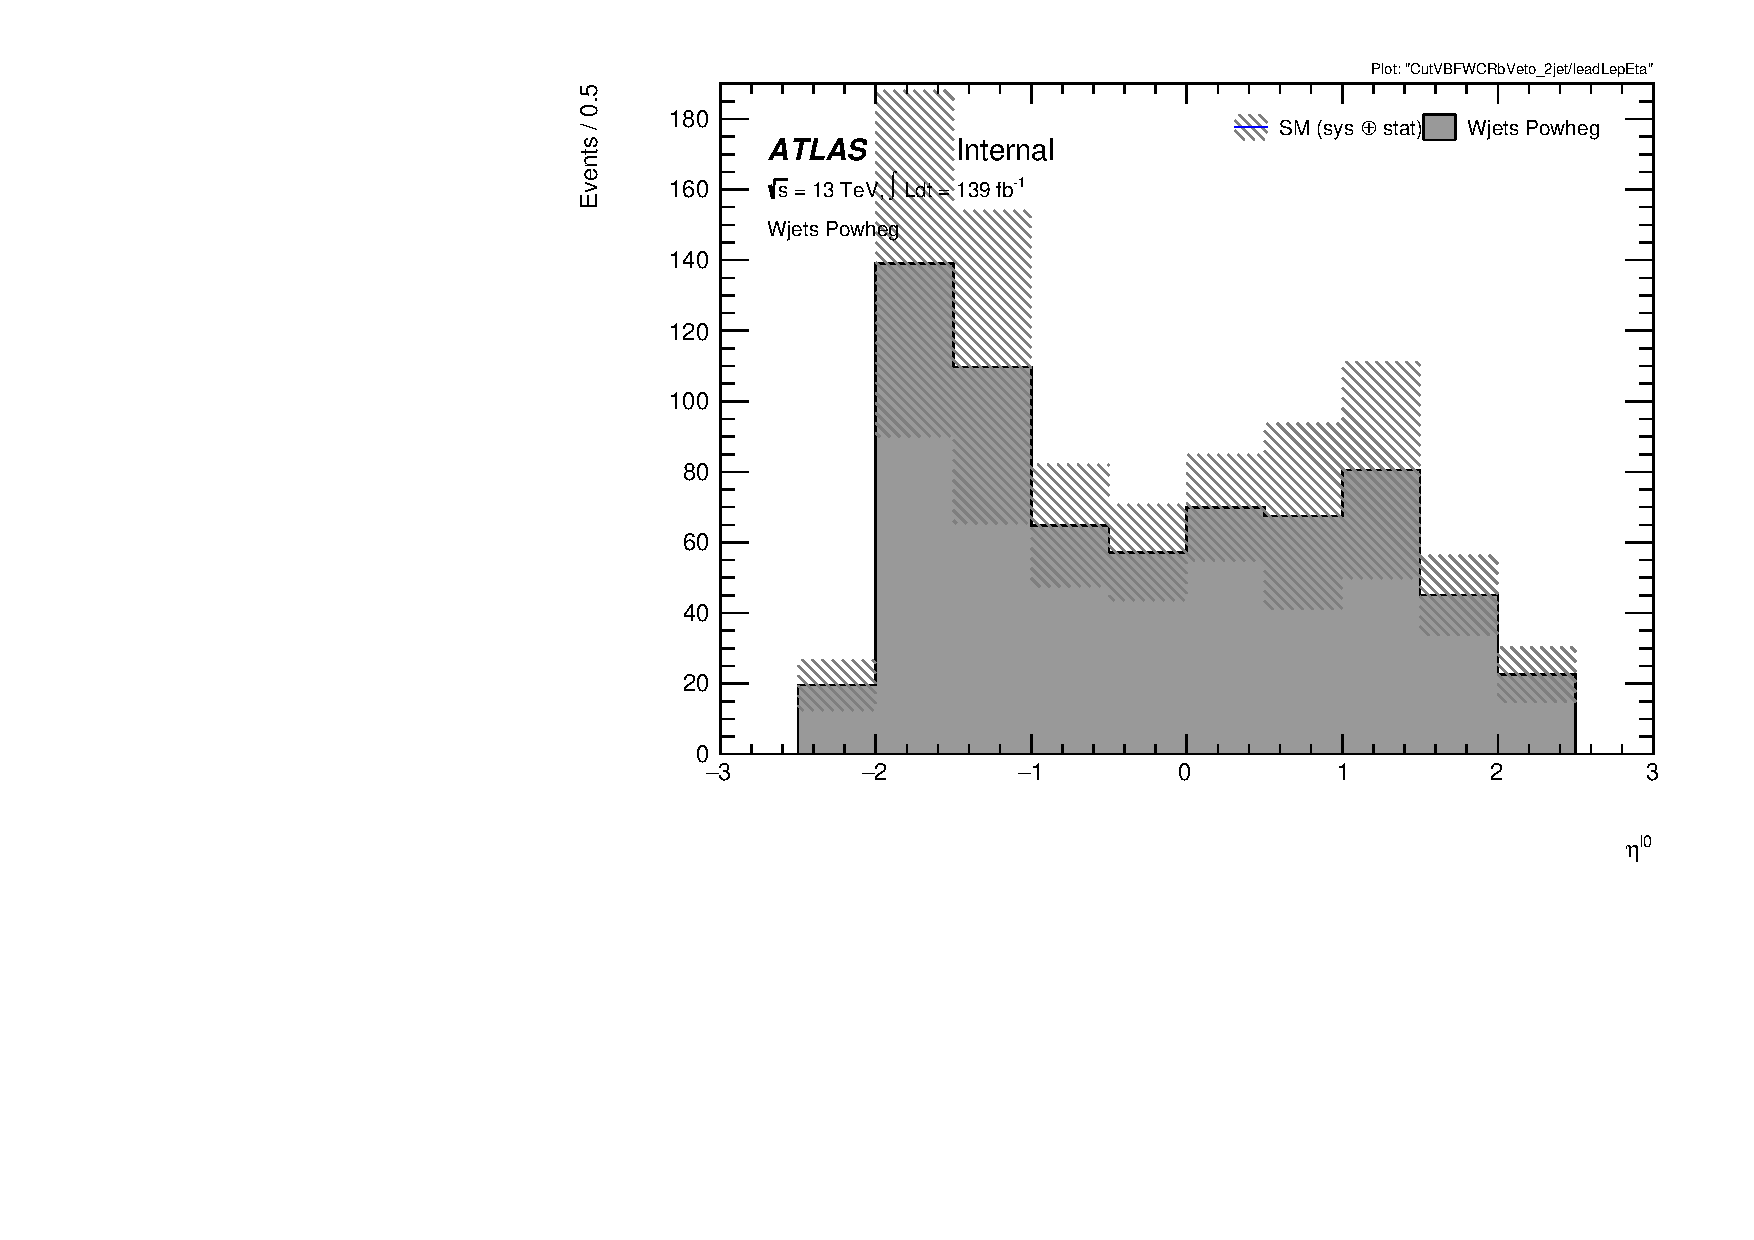
\includegraphics[width=0.23\textwidth]{FakeClosure/run2-emme-CutVBFWCRbVeto_2jet-leadLepEta-lin.pdf}
  }\hfill
  \subfloat[$\eta^{l1}$]{
      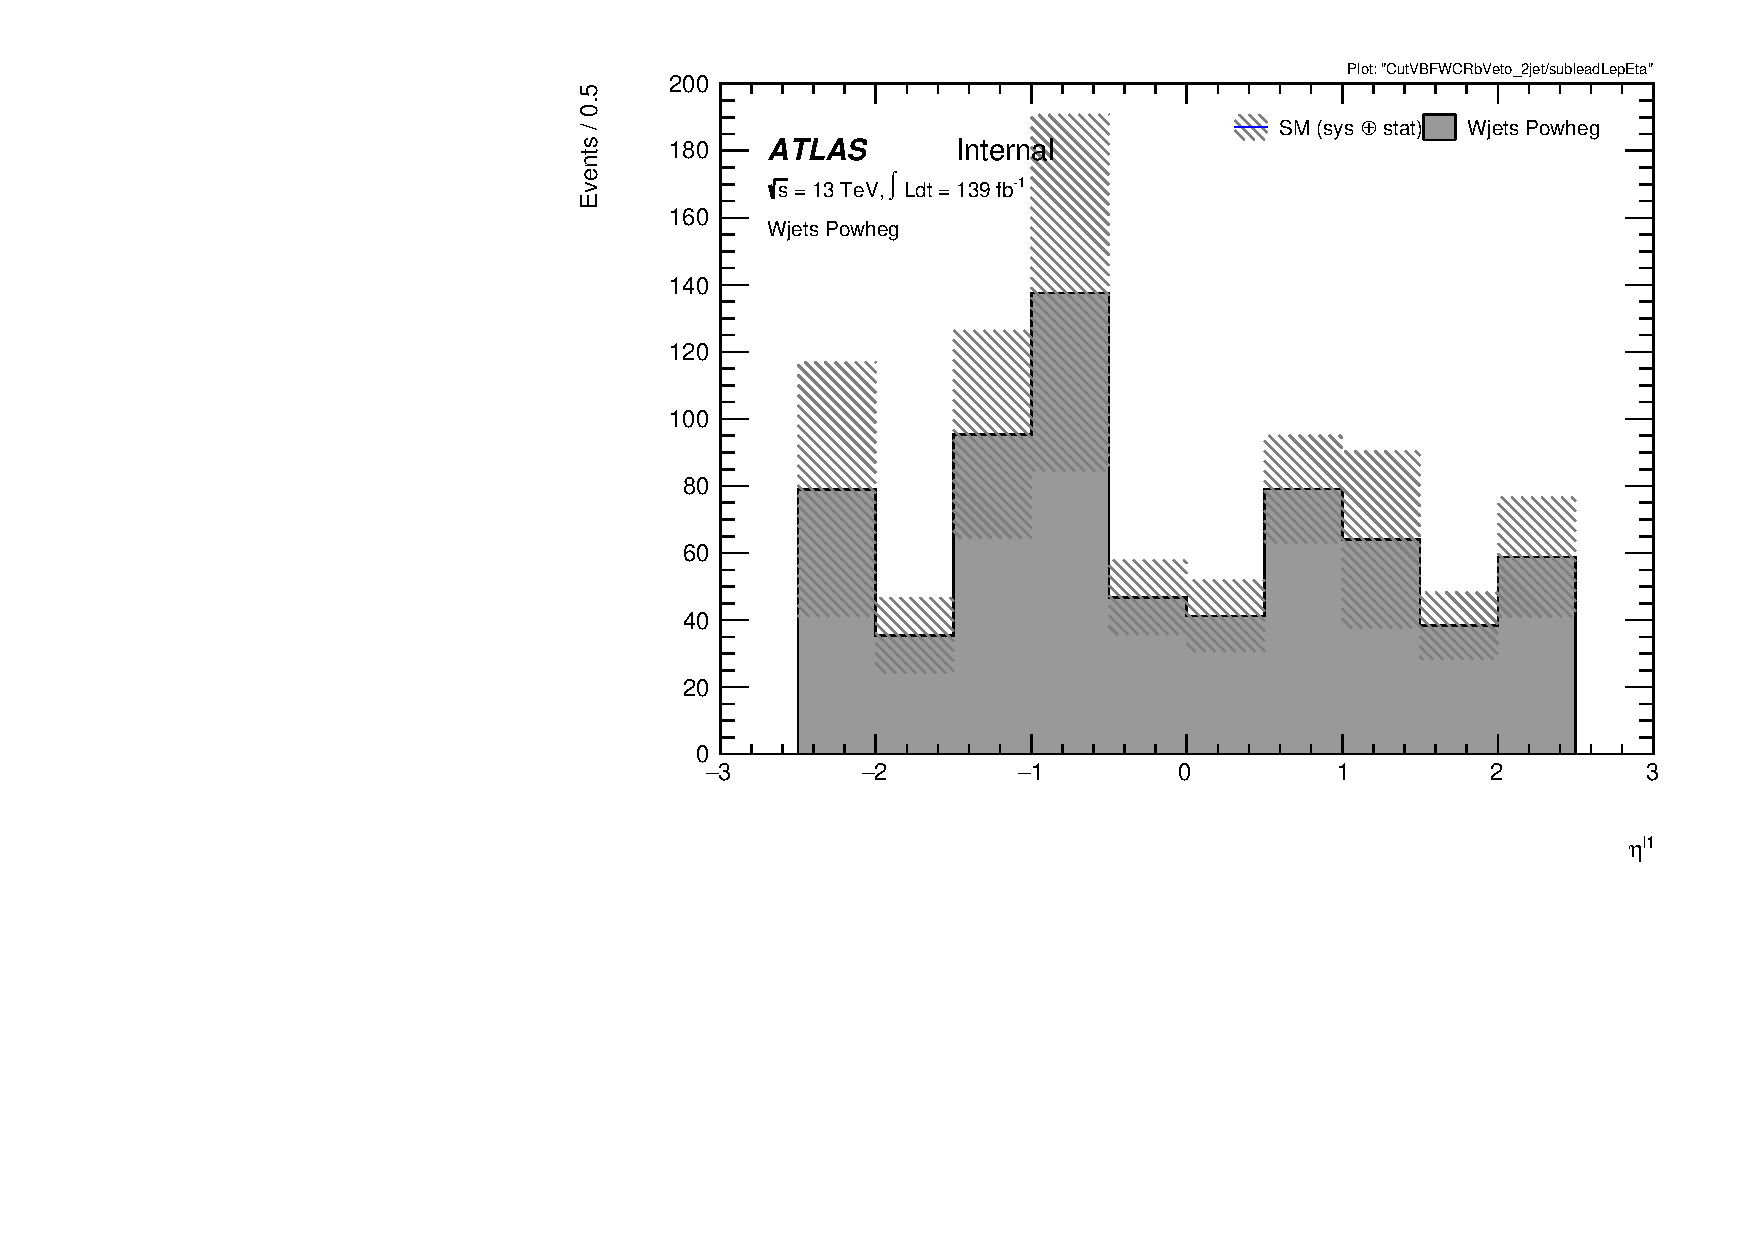
\includegraphics[width=0.23\textwidth]{FakeClosure/run2-emme-CutVBFWCRbVeto_2jet-subleadLepEta-lin.pdf}
  }\hfill
  \subfloat[$\eta^{j0}$]{
      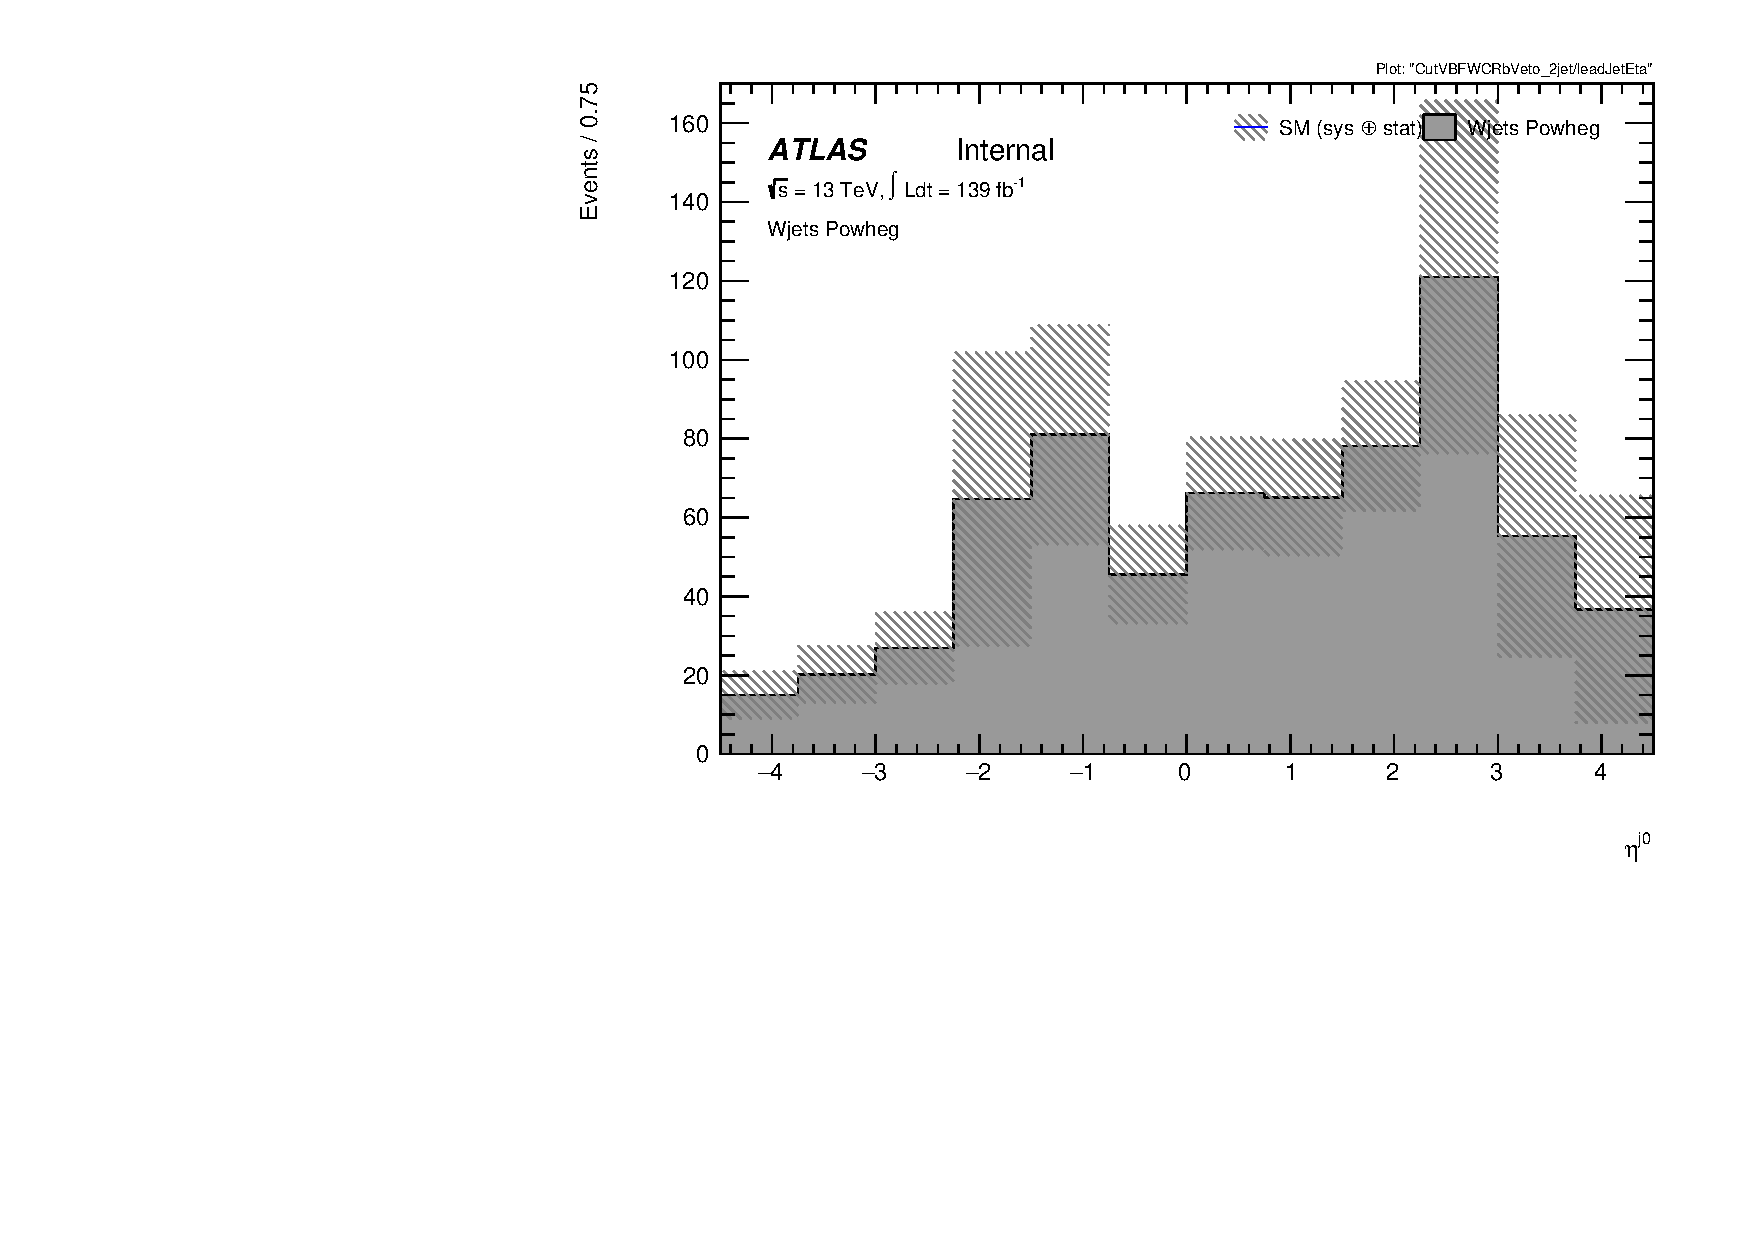
\includegraphics[width=0.23\textwidth]{FakeClosure/run2-emme-CutVBFWCRbVeto_2jet-leadJetEta-lin.pdf}
  }\hfill
  \subfloat[$\eta^{j1}$]{
      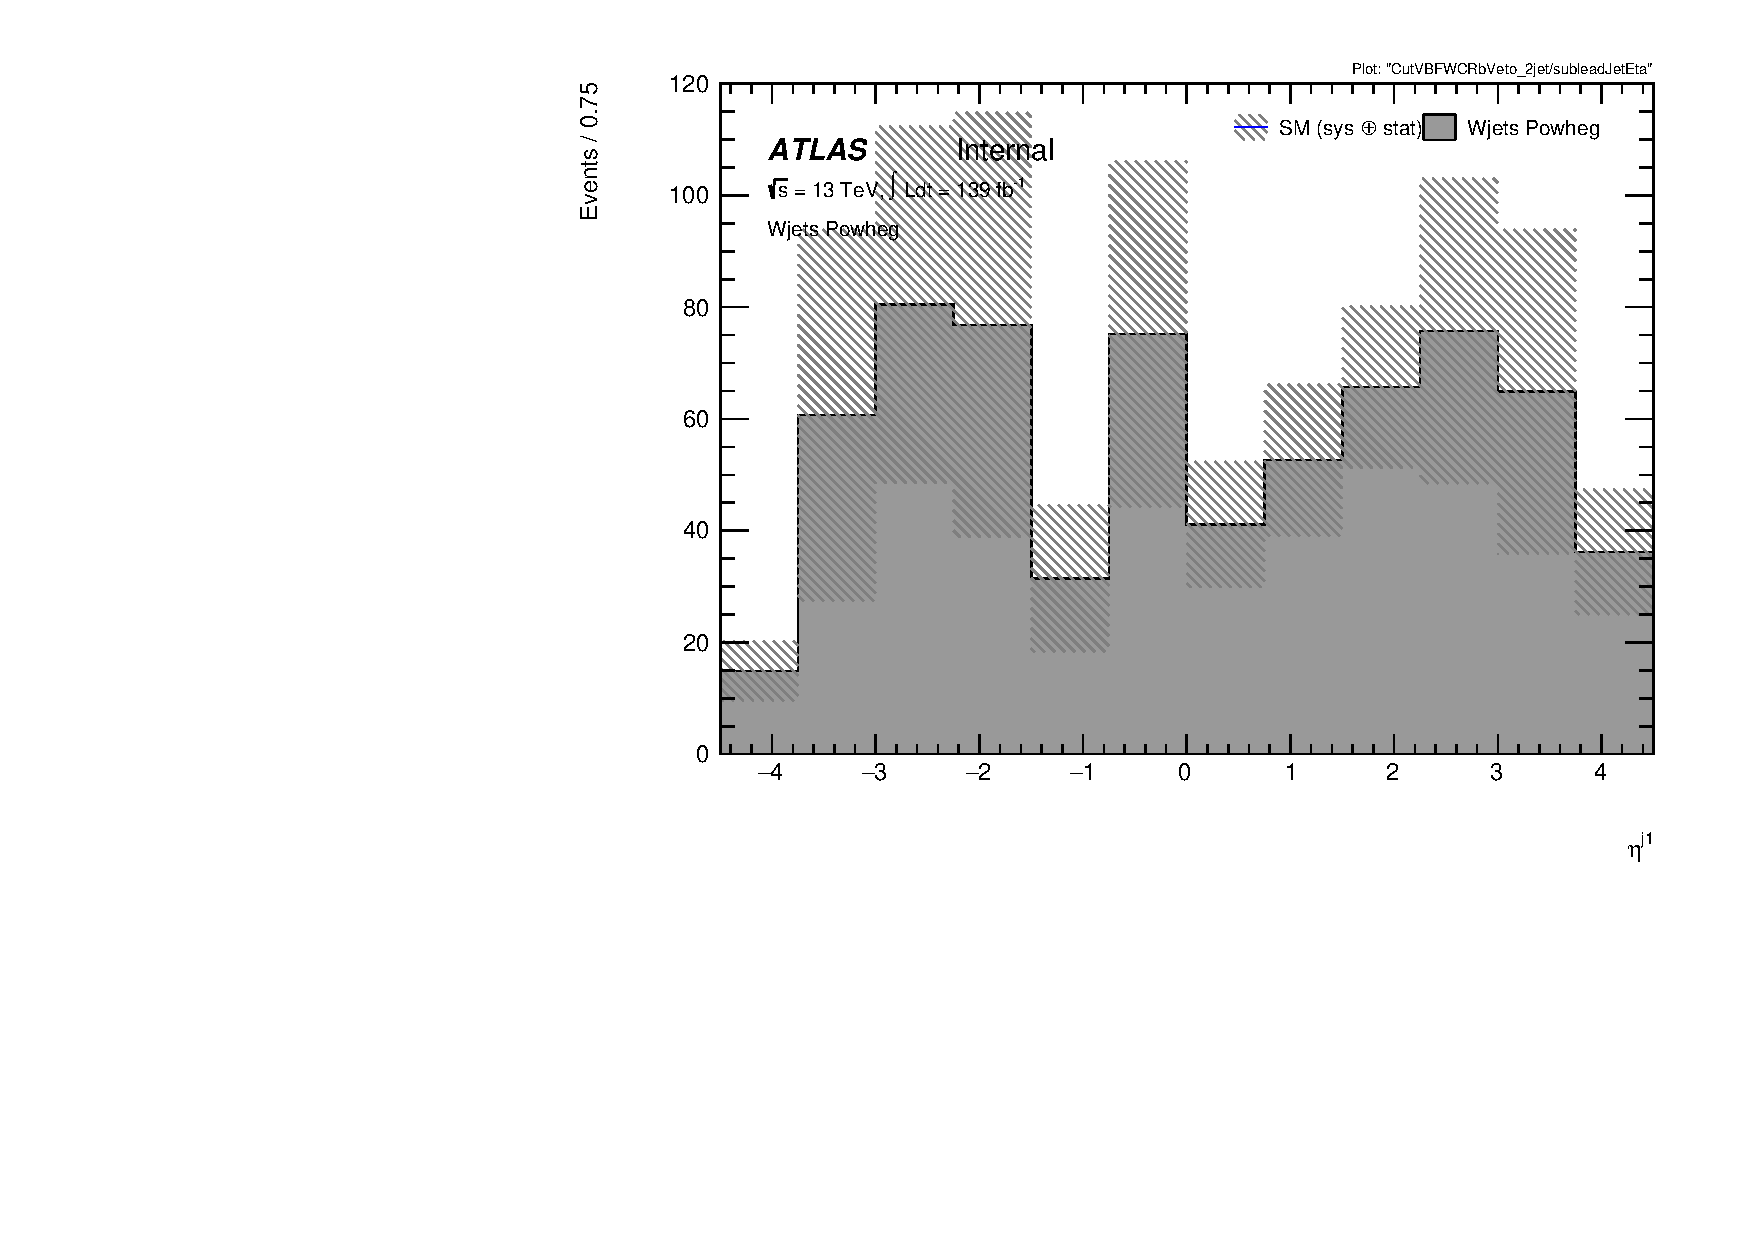
\includegraphics[width=0.23\textwidth]{FakeClosure/run2-emme-CutVBFWCRbVeto_2jet-subleadJetEta-lin.pdf}
  }%\hfill
{\caption{Distributions after preselection, FFs, 2-jets, and b-veto cuts for $W+$jets MC samples in the $W+$jets control region (id-anti-id).
\label{fig:WCR2jet}}}
\end{figure}

\begin{figure}[!h]
\centering
  \subfloat[$m_{jj}$]{
      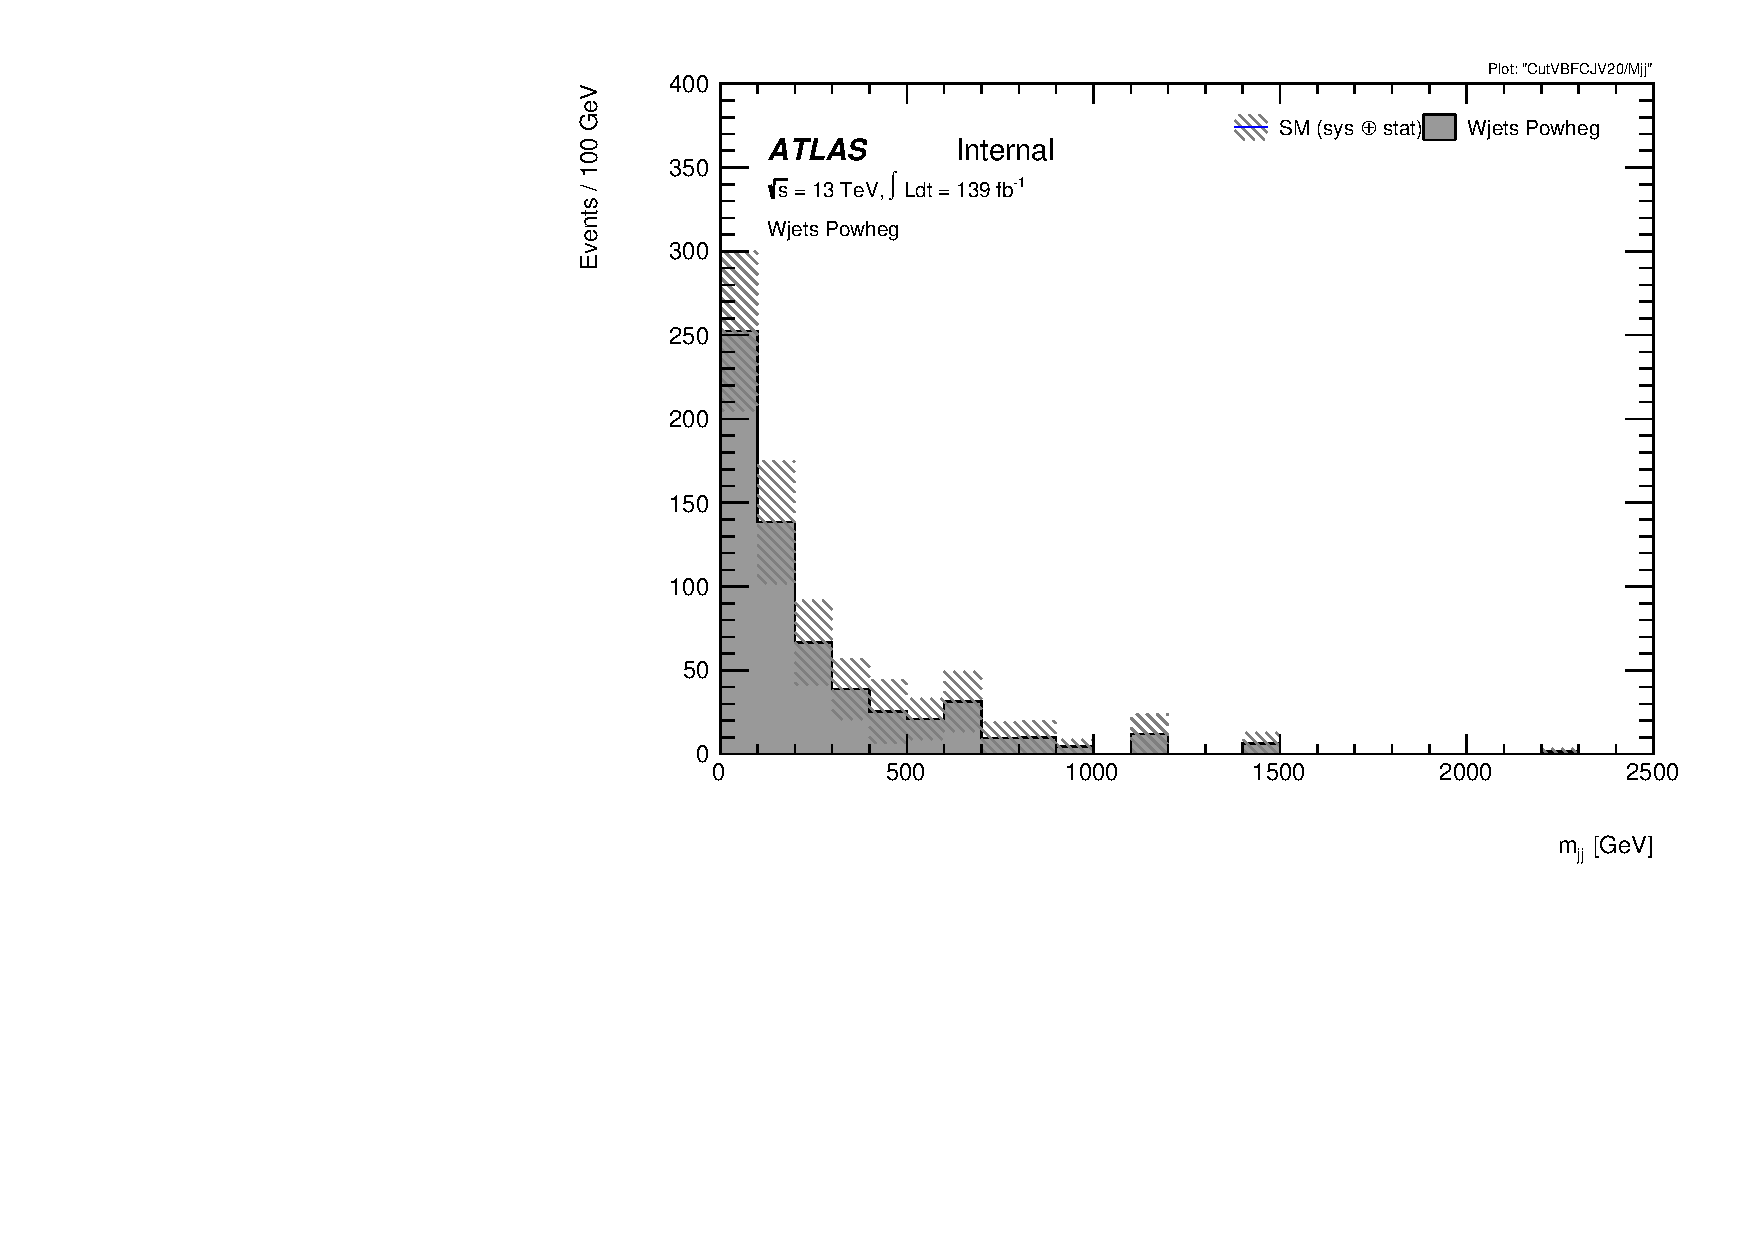
\includegraphics[width=0.3\textwidth]{FakeClosure/run2-emme-CutVBFCJV20-Mjj-lin.pdf}
  }\hfill
  \subfloat[$p^H_{T}$]{
      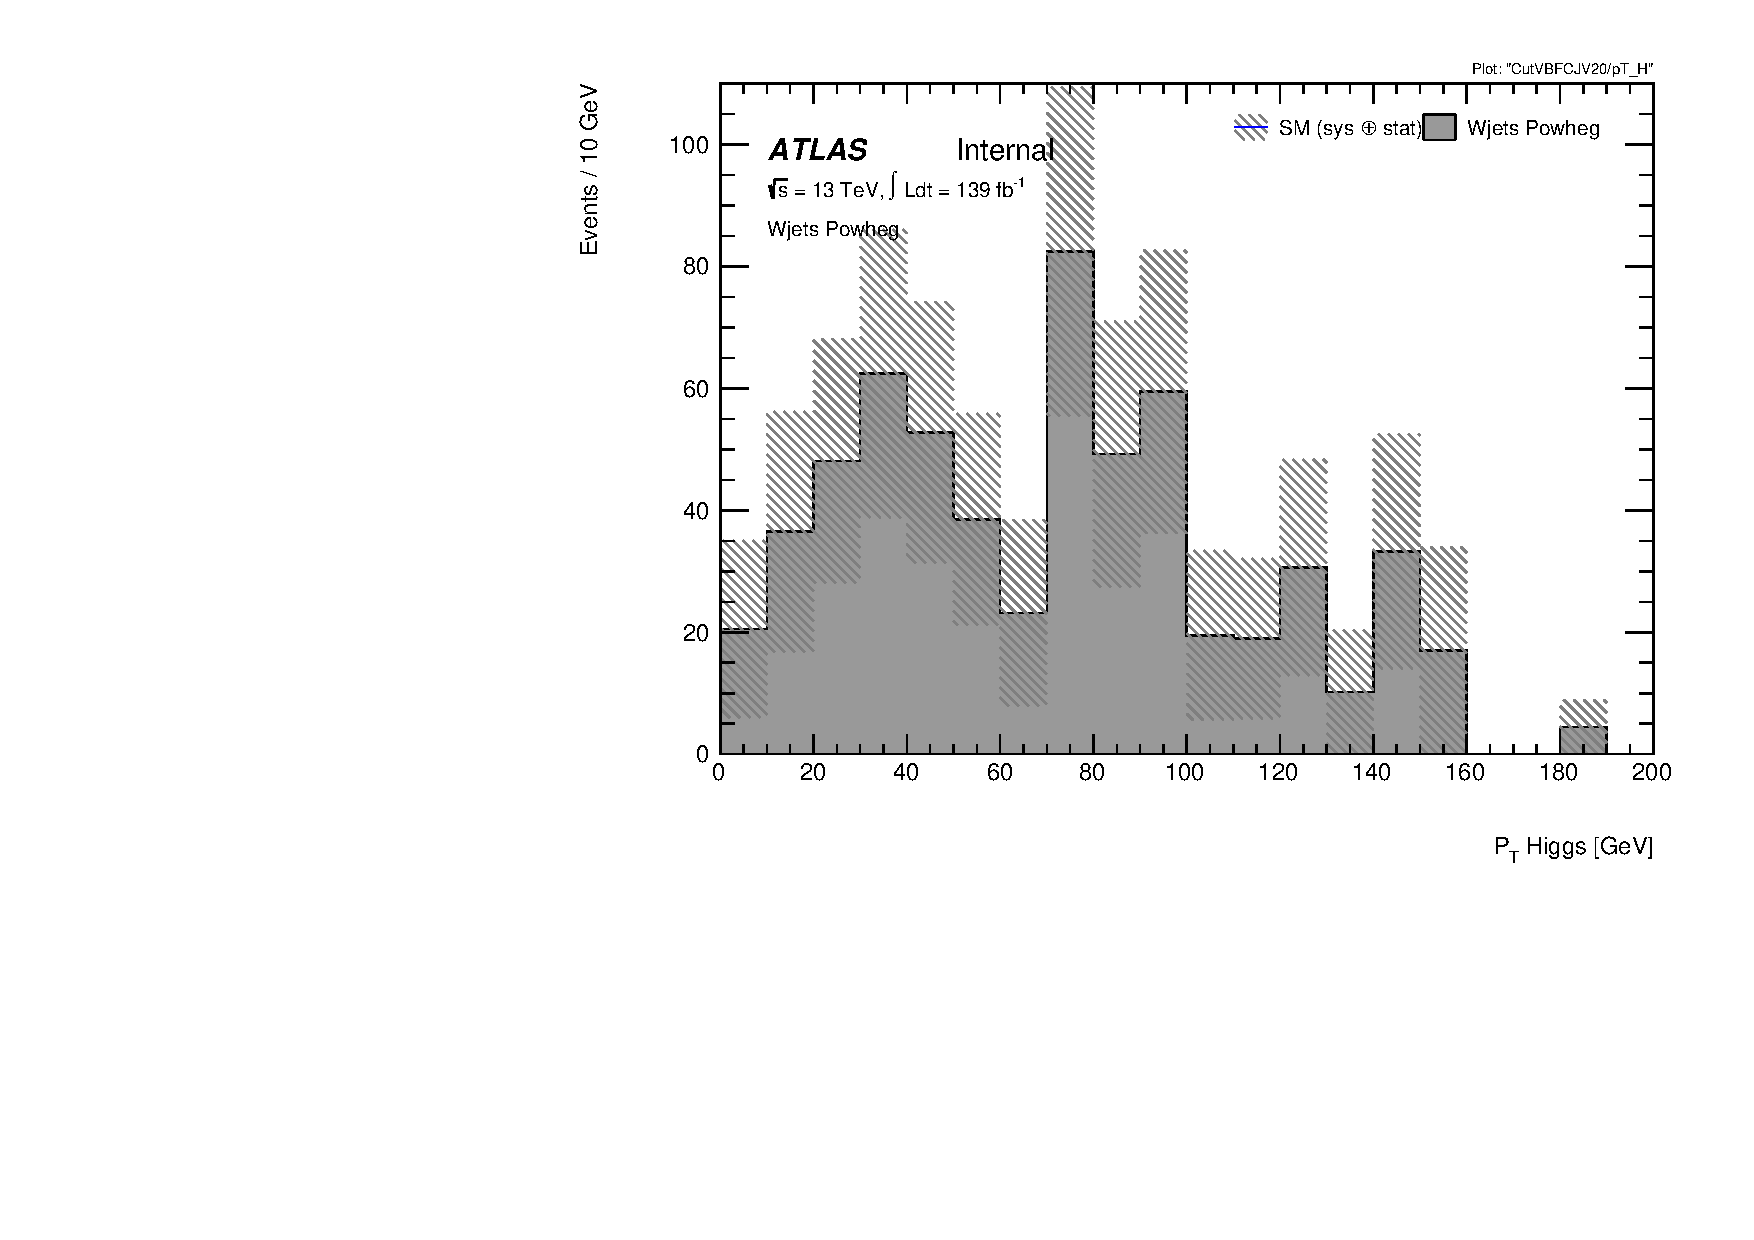
\includegraphics[width=0.3\textwidth]{FakeClosure/run2-emme-CutVBFCJV20-pT_H-lin.pdf}
  }\hfill
  \subfloat[$p_T^{l0}$]{
      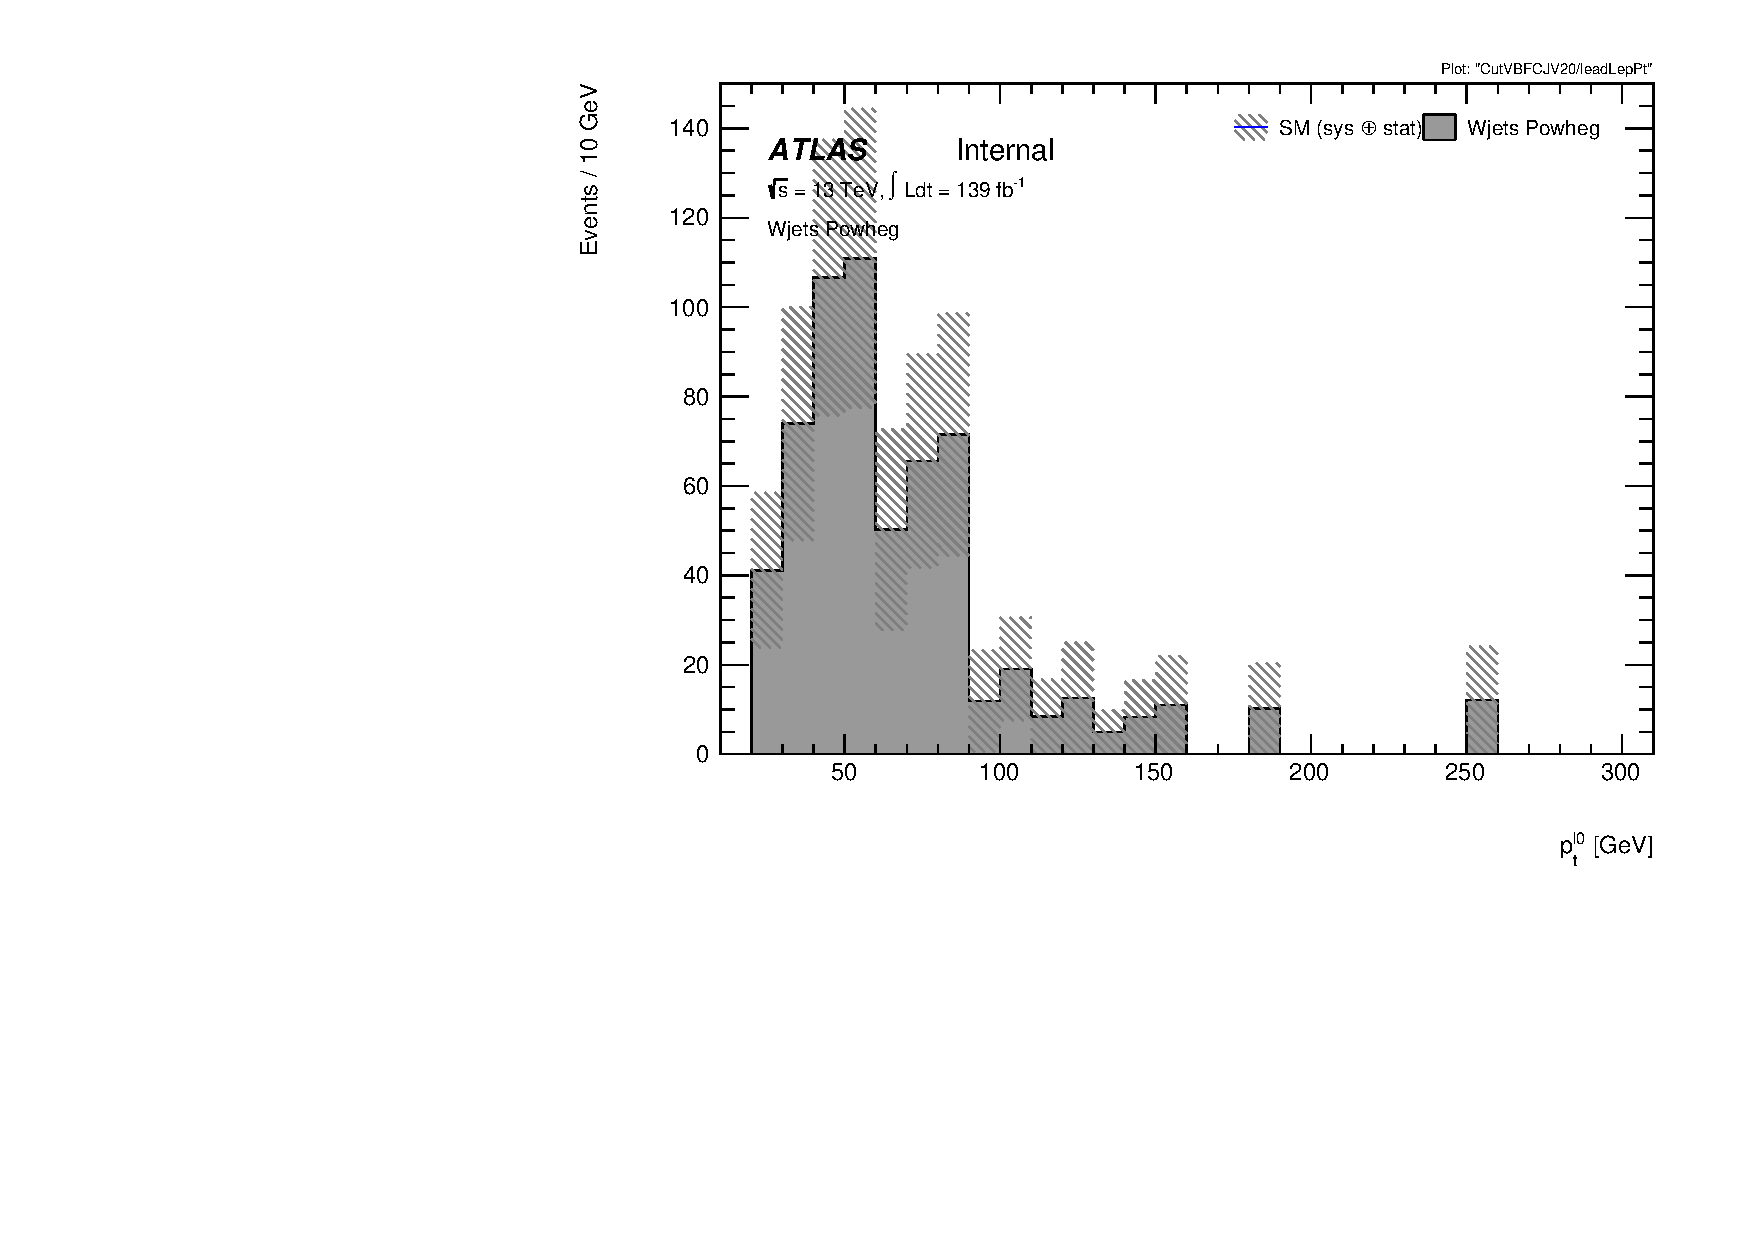
\includegraphics[width=0.3\textwidth]{FakeClosure/run2-emme-CutVBFCJV20-leadLepPt-lin.pdf}
  }\hfill
  \subfloat[$p_T^{l1}$]{
      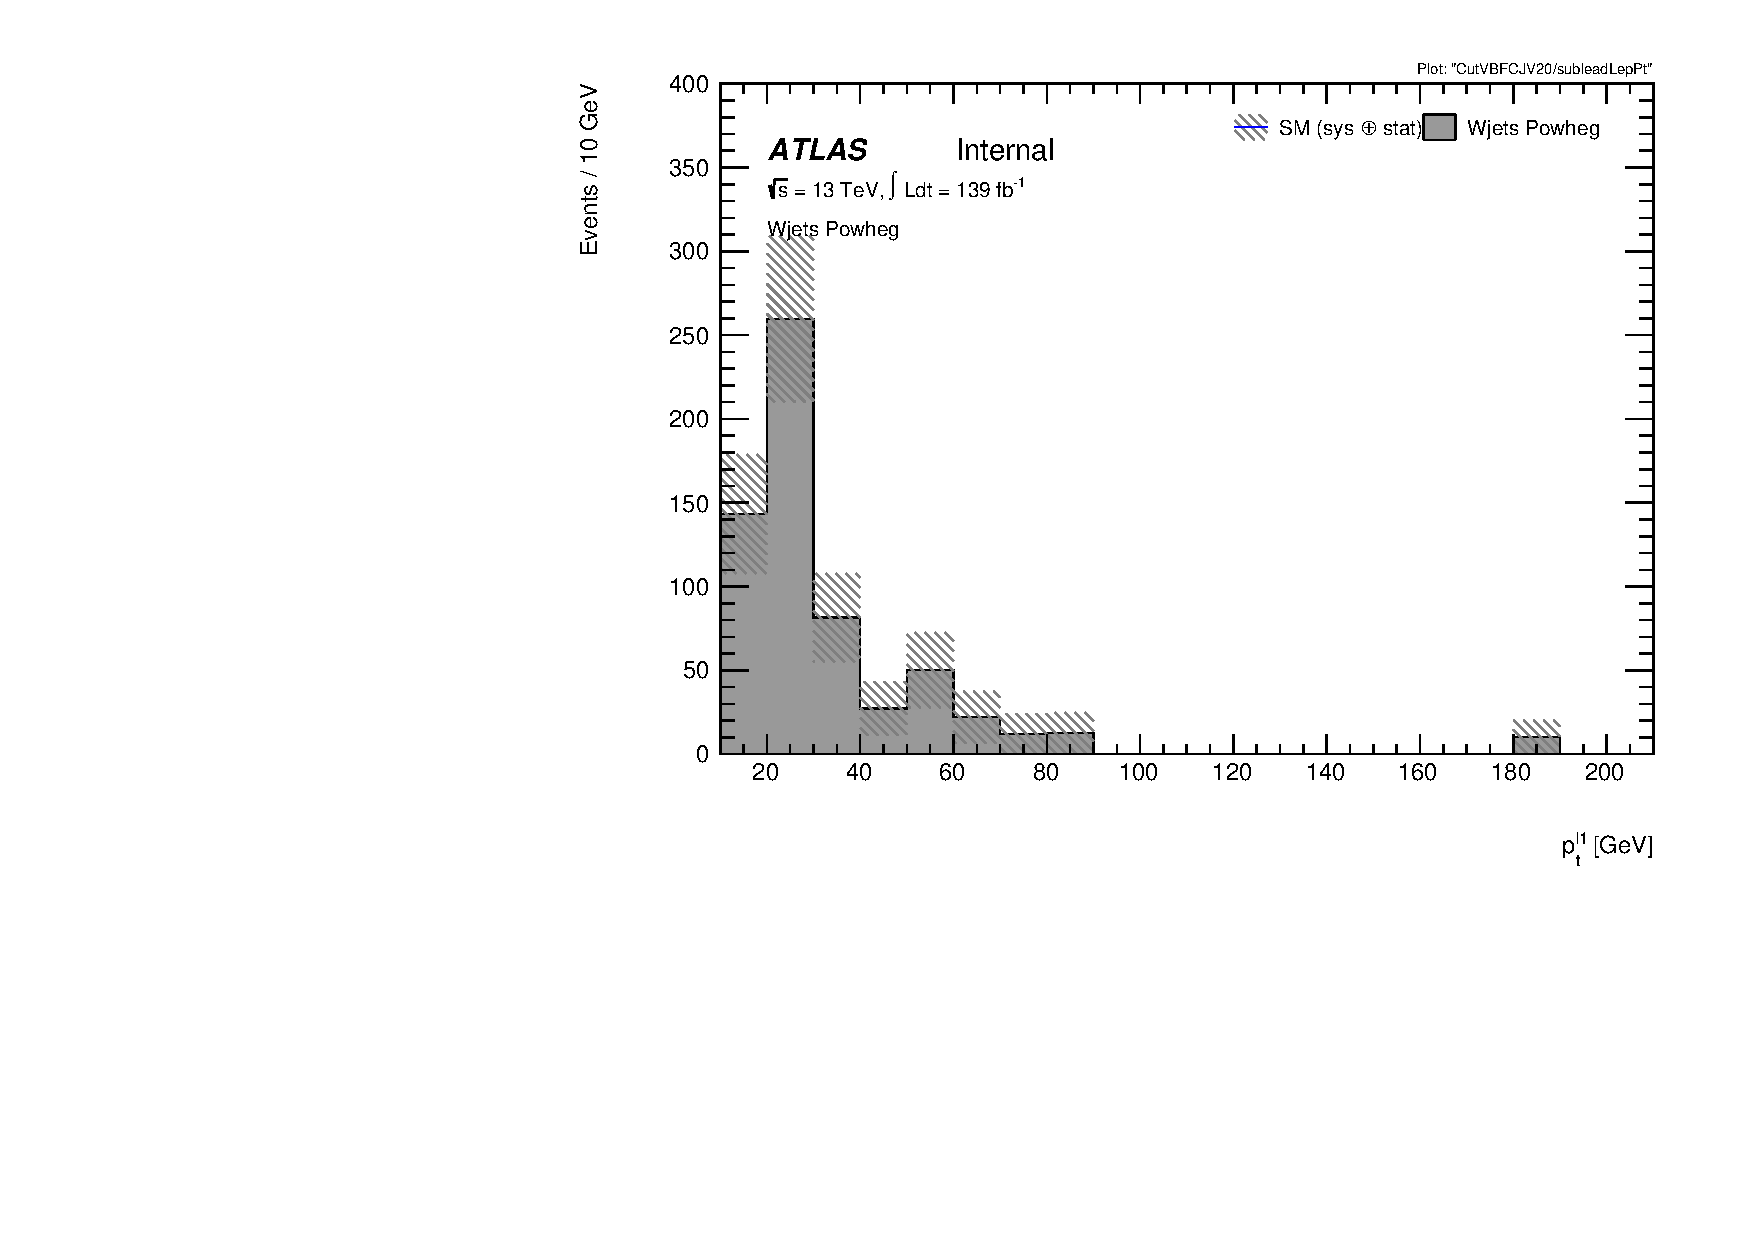
\includegraphics[width=0.3\textwidth]{FakeClosure/run2-emme-CutVBFCJV20-subleadLepPt-lin.pdf}
  }\hfill
  \subfloat[$p_T^{j0}$]{
      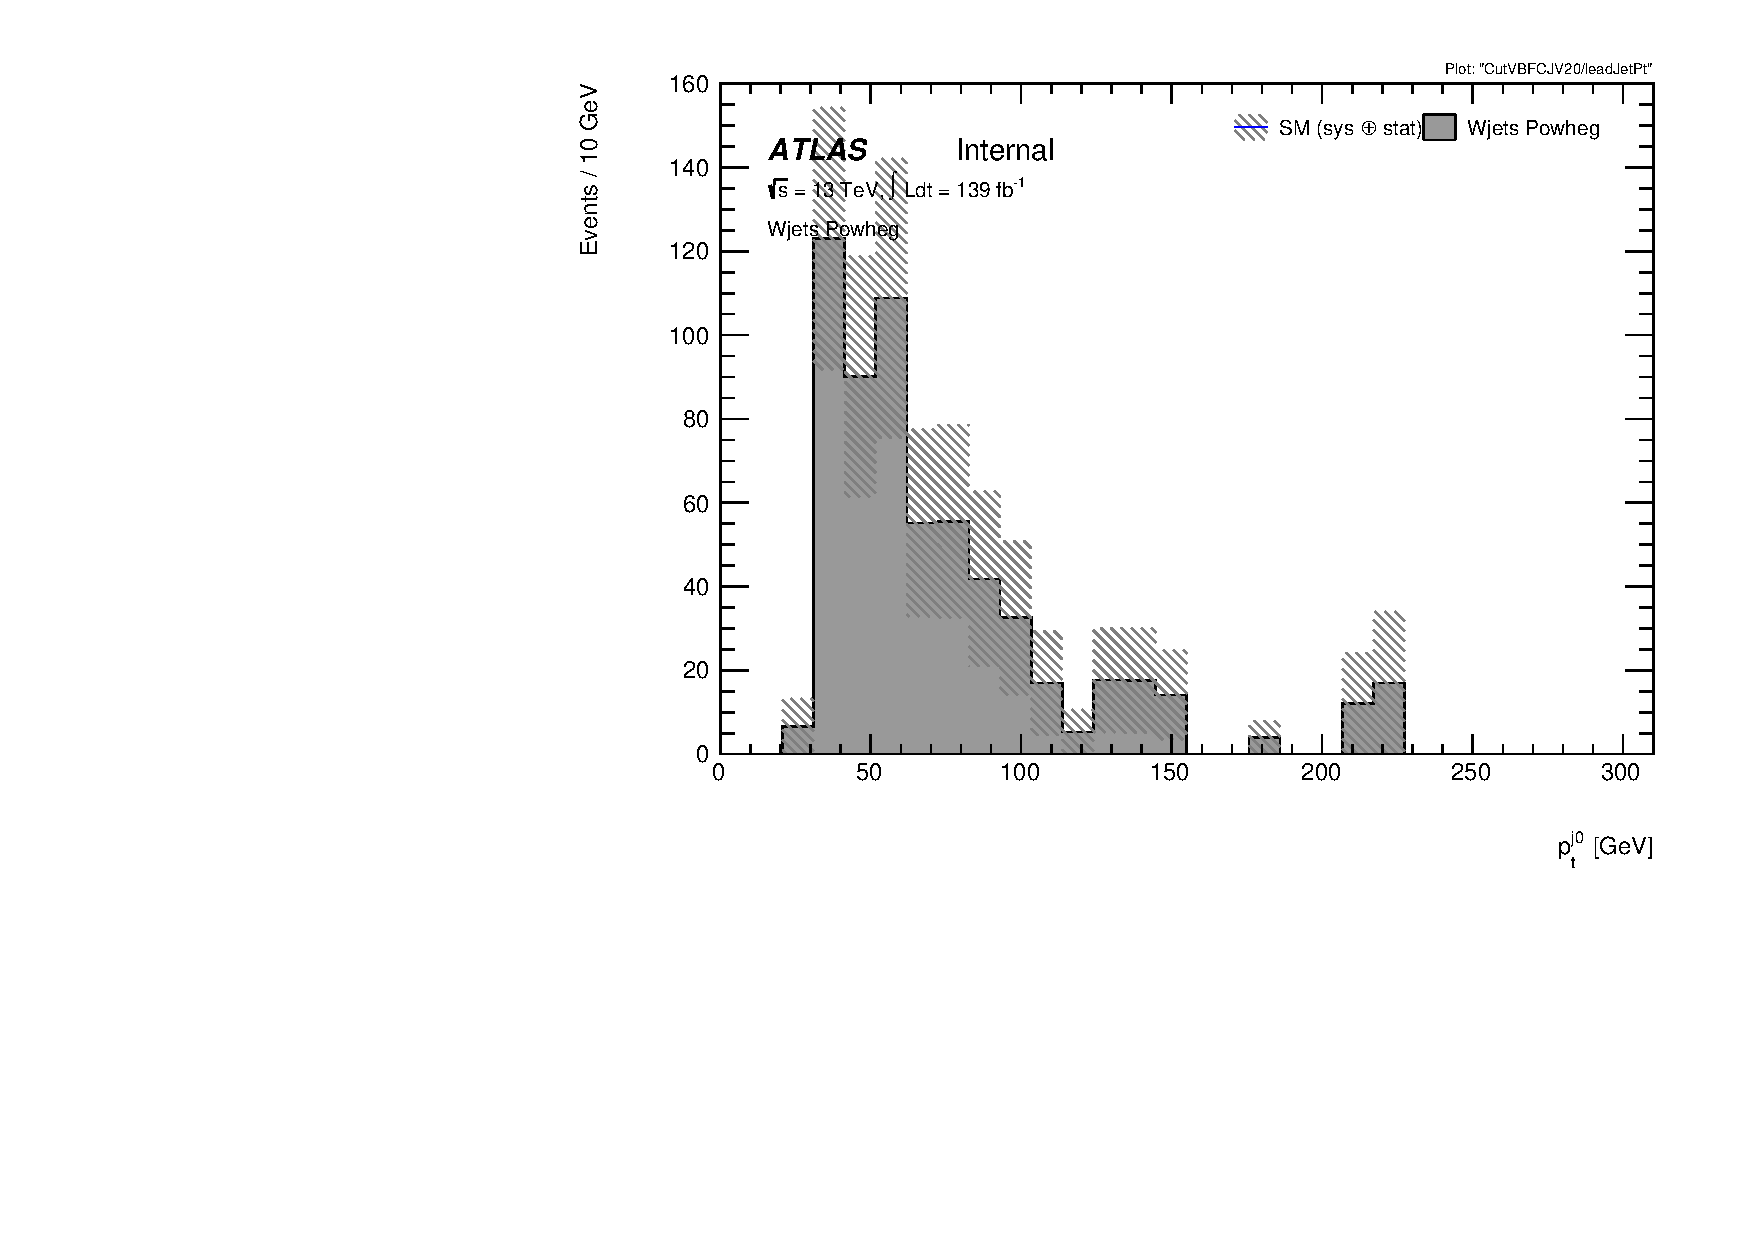
\includegraphics[width=0.3\textwidth]{FakeClosure/run2-emme-CutVBFCJV20-leadJetPt-lin.pdf}
  }\hfill
  \subfloat[$p_T^{j1}$]{
      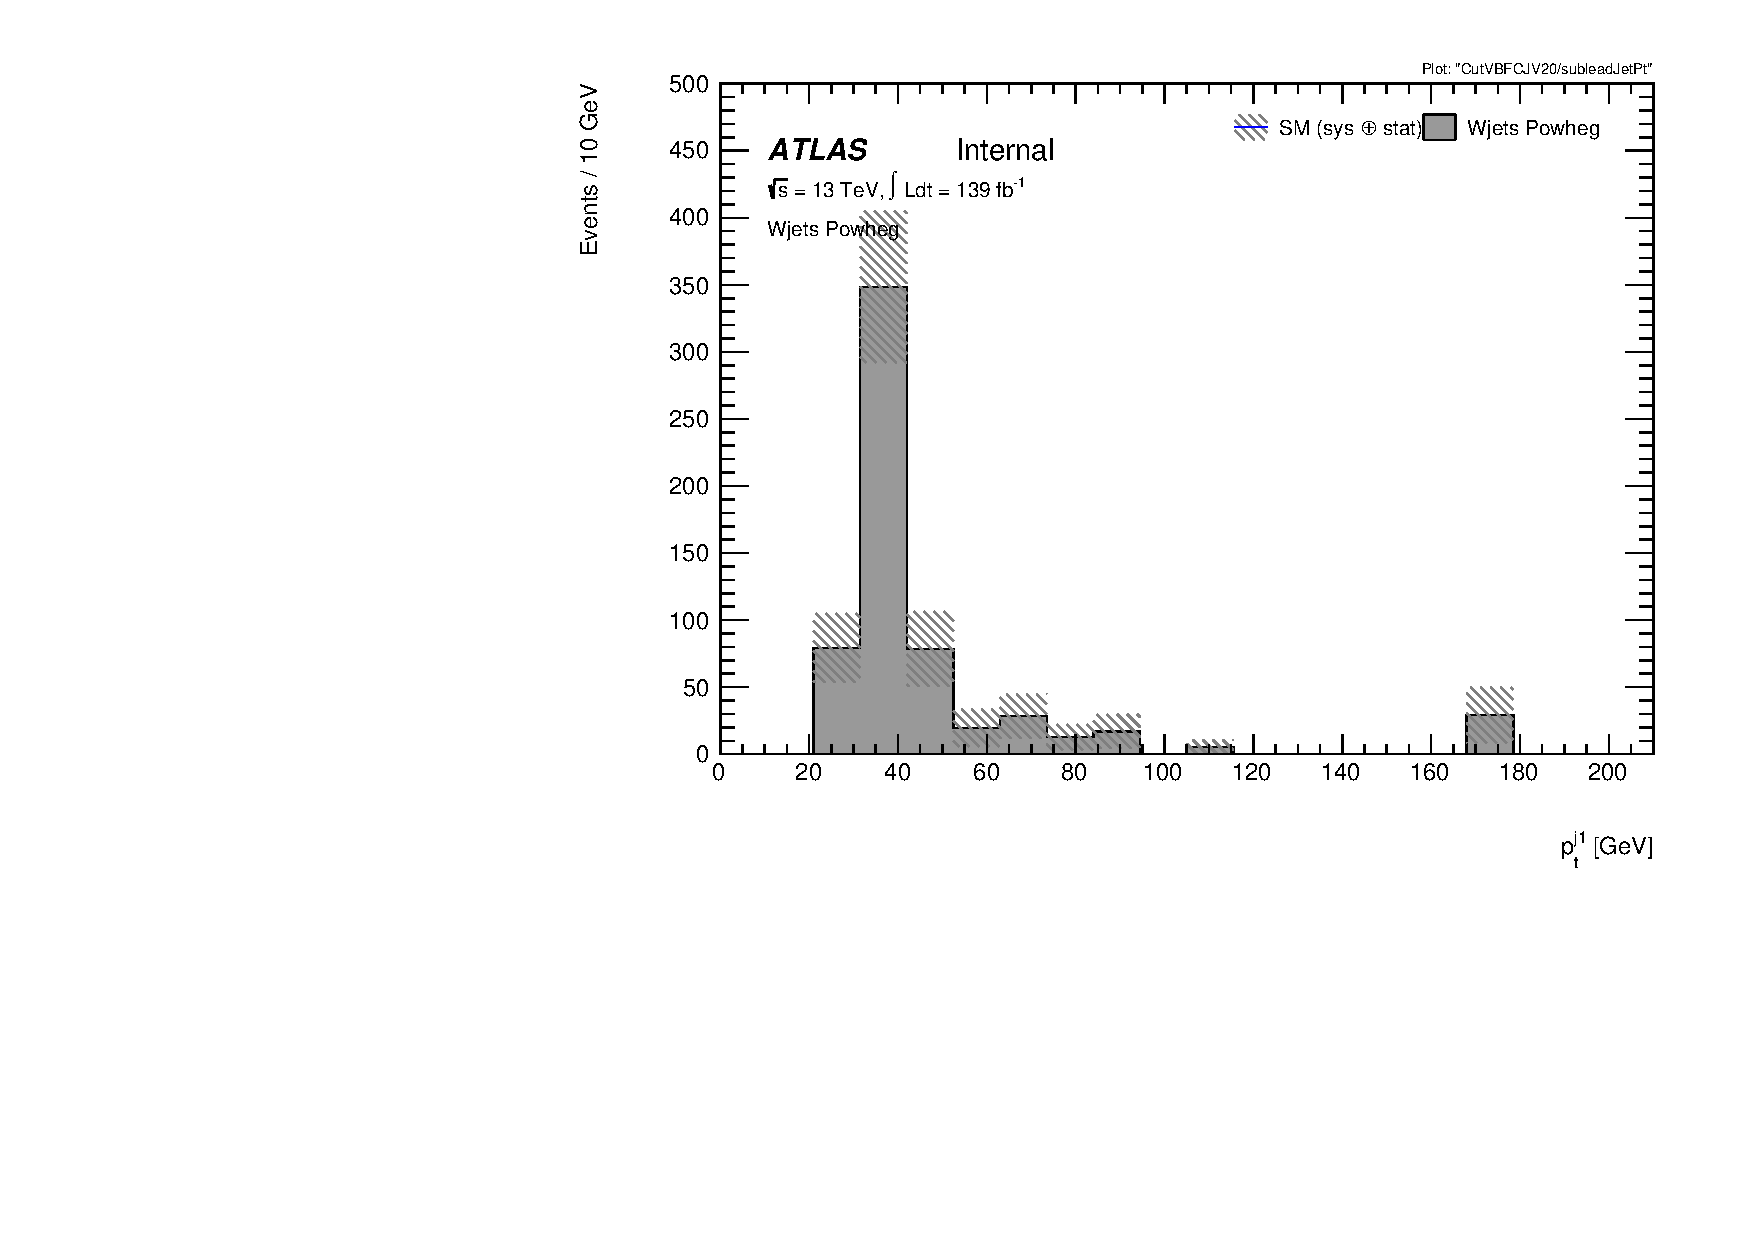
\includegraphics[width=0.3\textwidth]{FakeClosure/run2-emme-CutVBFCJV20-subleadJetPt-lin.pdf}
  }\hfill
  \subfloat[$\eta^{l0}$]{
      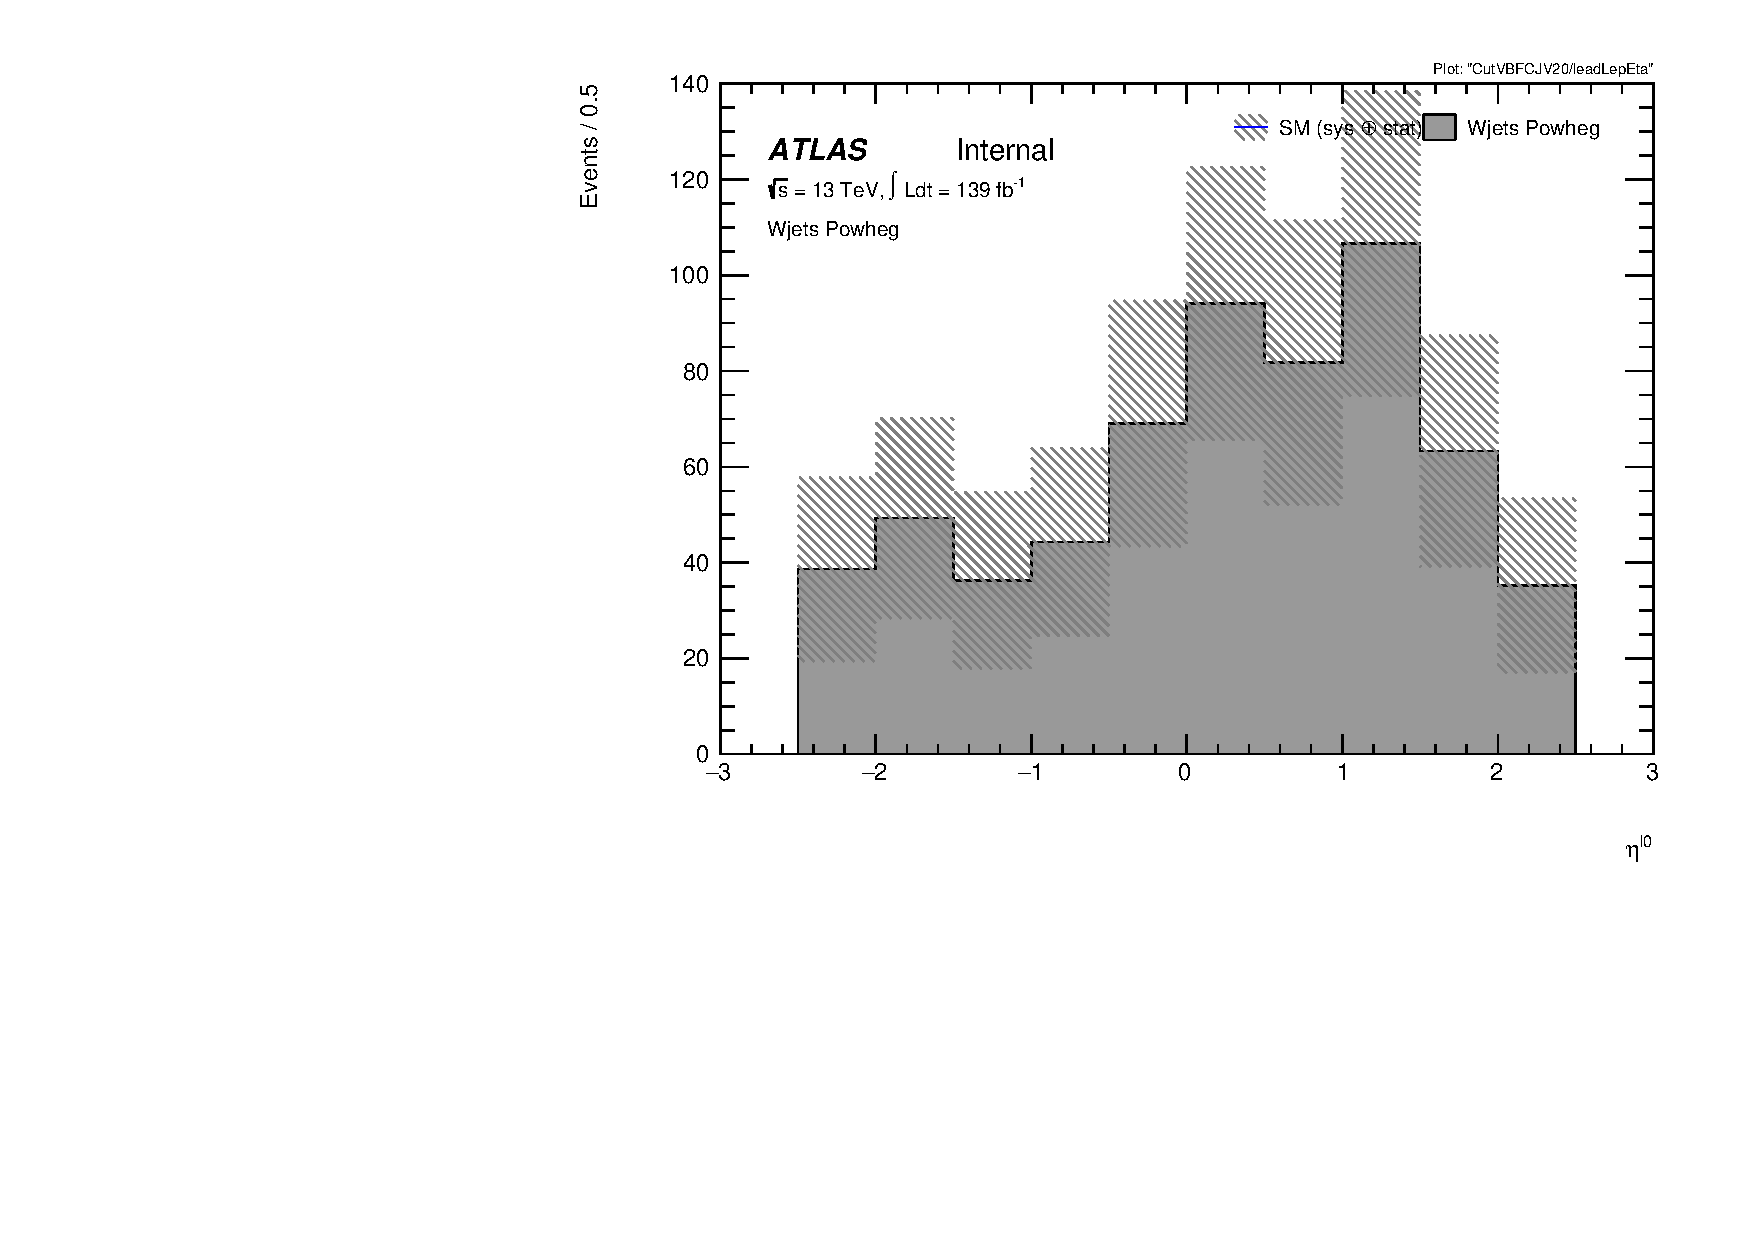
\includegraphics[width=0.23\textwidth]{FakeClosure/run2-emme-CutVBFCJV20-leadLepEta-lin.pdf}
  }\hfill
  \subfloat[$\eta^{l1}$]{
      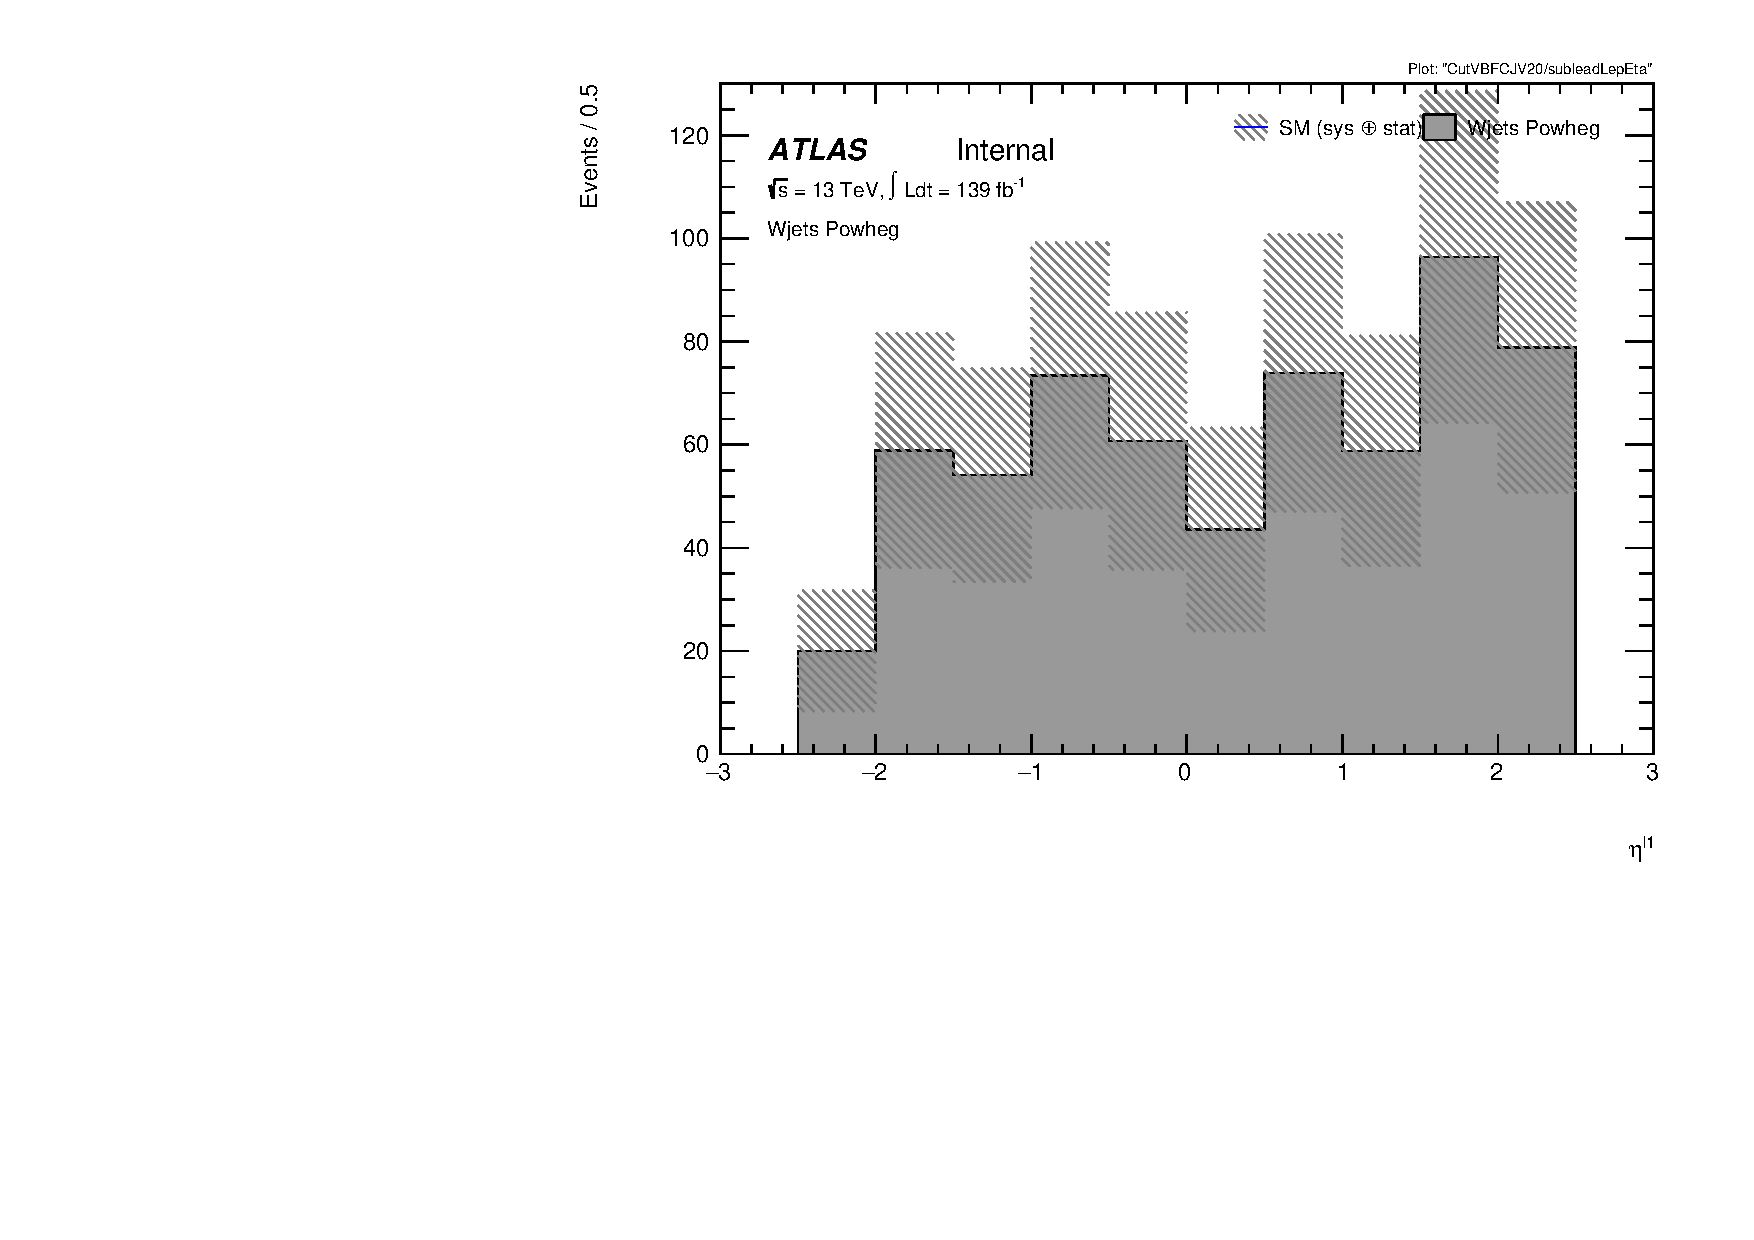
\includegraphics[width=0.23\textwidth]{FakeClosure/run2-emme-CutVBFCJV20-subleadLepEta-lin.pdf}
  }\hfill
  \subfloat[$\eta^{j0}$]{
      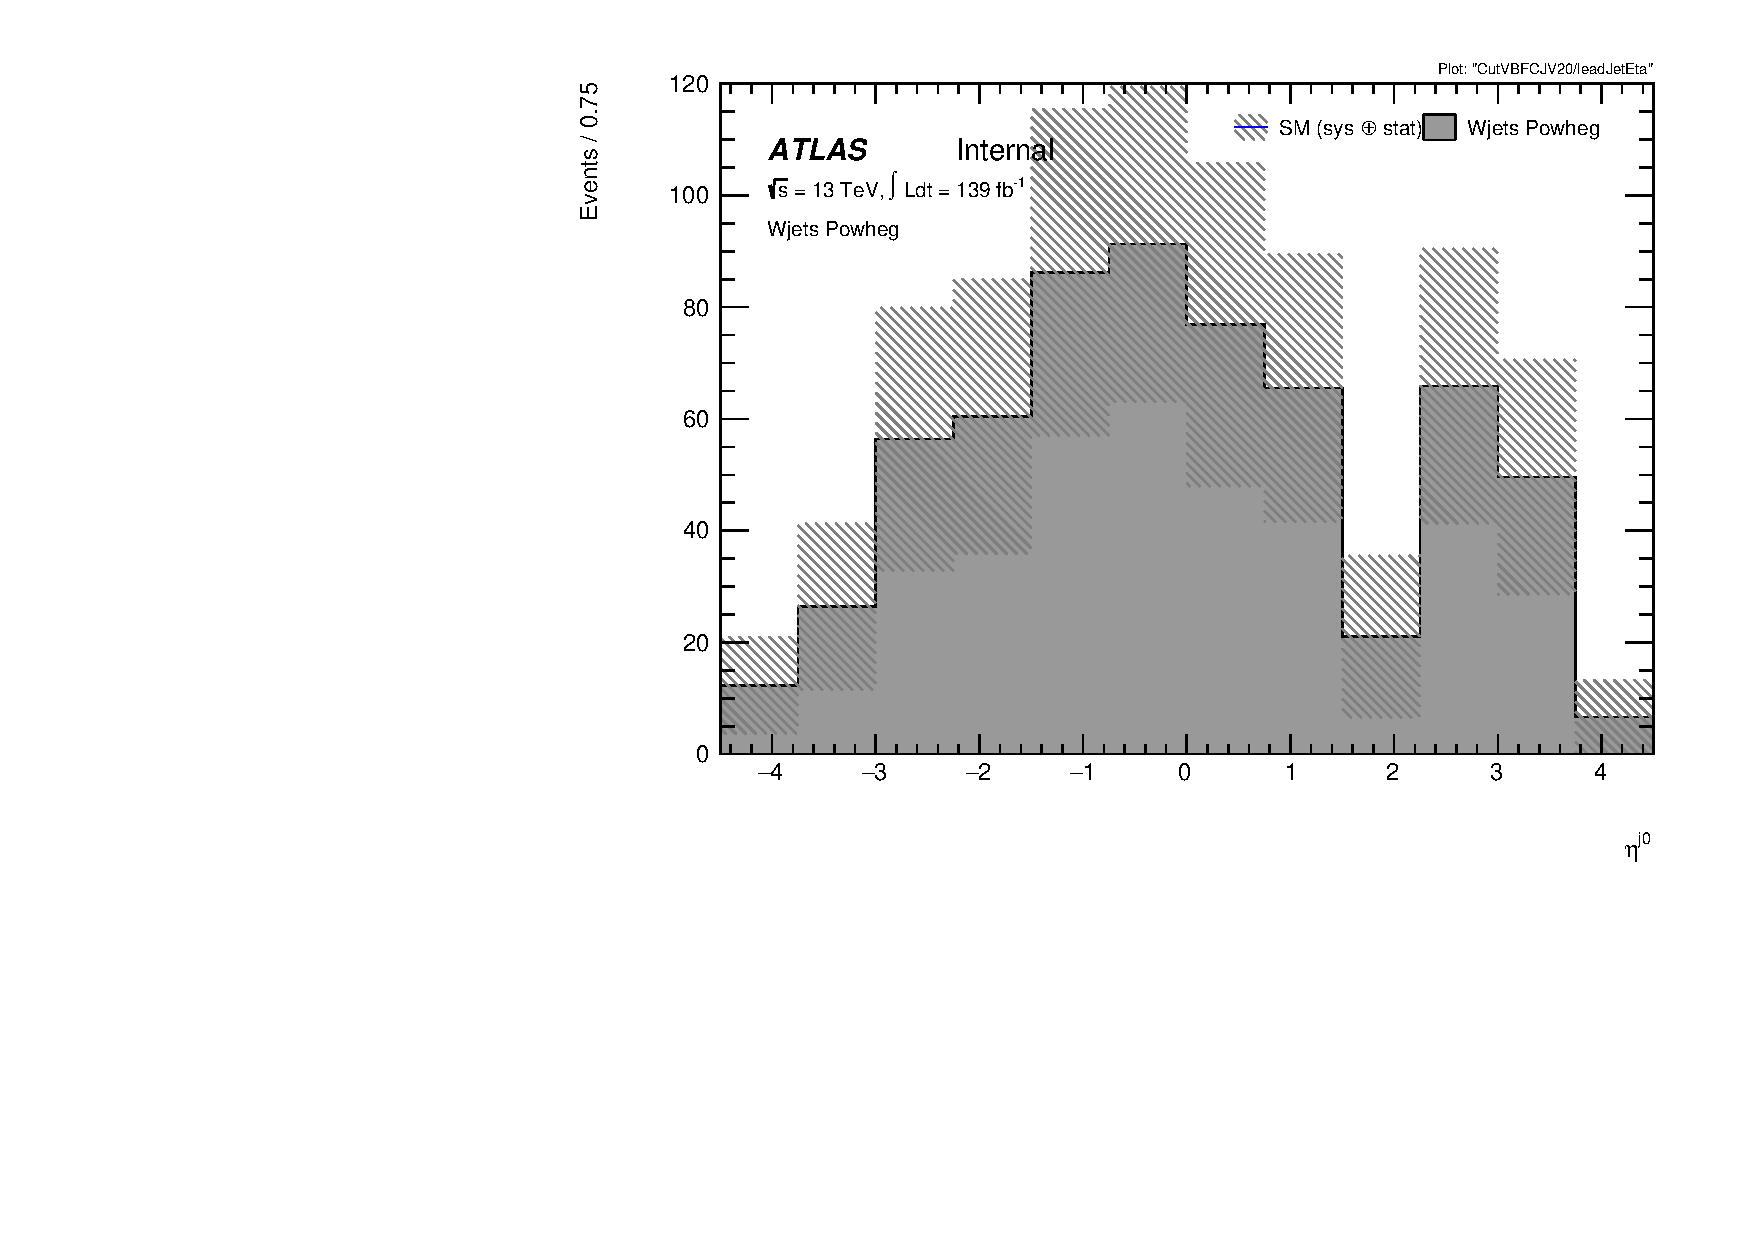
\includegraphics[width=0.23\textwidth]{FakeClosure/run2-emme-CutVBFCJV20-leadJetEta-lin.pdf}
  }\hfill
  \subfloat[$\eta^{j1}$]{
      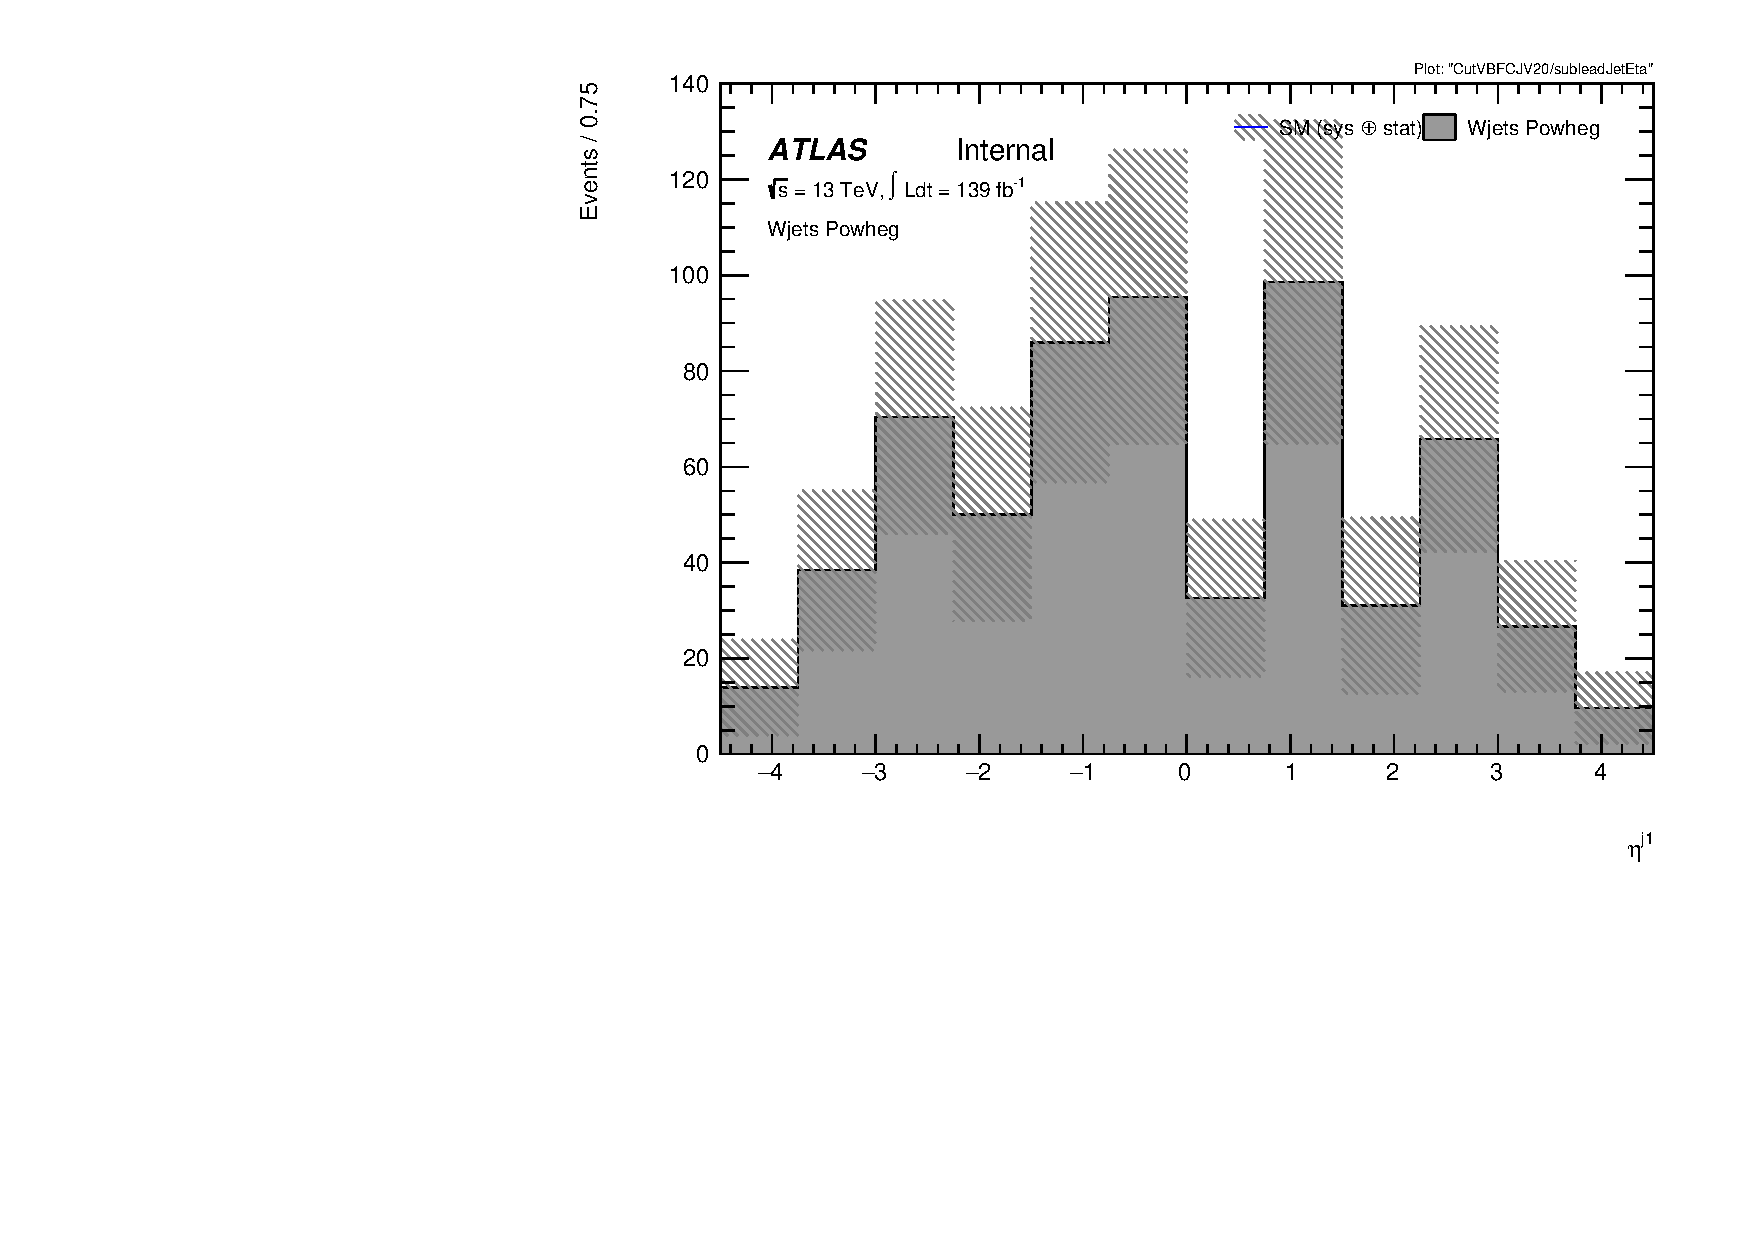
\includegraphics[width=0.23\textwidth]{FakeClosure/run2-emme-CutVBFCJV20-subleadJetEta-lin.pdf}
  }%\hfill
{\caption{Distributions after preselection, 2-jets, b-veto and CJV cuts for $W+$jets MC samples in the signal region (id-id).
\label{fig:SR2jet}}}
\end{figure}


\begin{figure}[!h]
\centering
  \subfloat[$m_{jj}$]{
      \includegraphics[width=0.3\textwidth]{FakeClosure/run2-emme-CutVBFWCRCJV20-Mjj-lin.pdf}
  }\hfill
  \subfloat[$p^H_{T}$]{
      \includegraphics[width=0.3\textwidth]{FakeClosure/run2-emme-CutVBFWCRCJV20-pT_H-lin.pdf}
  }\hfill
  \subfloat[$p_T^{l0}$]{
      \includegraphics[width=0.3\textwidth]{FakeClosure/run2-emme-CutVBFWCRCJV20-leadLepPt-lin.pdf}
  }\hfill
  \subfloat[$p_T^{l1}$]{
      \includegraphics[width=0.3\textwidth]{FakeClosure/run2-emme-CutVBFWCRCJV20-subleadLepPt-lin.pdf}
  }\hfill
  \subfloat[$p_T^{j0}$]{
      \includegraphics[width=0.3\textwidth]{FakeClosure/run2-emme-CutVBFWCRCJV20-leadJetPt-lin.pdf}
  }\hfill
  \subfloat[$p_T^{j1}$]{
      \includegraphics[width=0.3\textwidth]{FakeClosure/run2-emme-CutVBFWCRCJV20-subleadJetPt-lin.pdf}
  }\hfill
  \subfloat[$\eta^{l0}$]{
      \includegraphics[width=0.23\textwidth]{FakeClosure/run2-emme-CutVBFWCRCJV20-leadLepEta-lin.pdf}
  }\hfill
  \subfloat[$\eta^{l1}$]{
      \includegraphics[width=0.23\textwidth]{FakeClosure/run2-emme-CutVBFWCRCJV20-subleadLepEta-lin.pdf}
  }\hfill
  \subfloat[$\eta^{j0}$]{
      \includegraphics[width=0.23\textwidth]{FakeClosure/run2-emme-CutVBFWCRCJV20-leadJetEta-lin.pdf}
  }\hfill
  \subfloat[$\eta^{j1}$]{
      \includegraphics[width=0.23\textwidth]{FakeClosure/run2-emme-CutVBFWCRCJV20-subleadJetEta-lin.pdf}
  }%\hfill
{\caption{Distributions after preselection, FFs, 2-jets, b-veto and CJV cuts for $W+$jets MC samples in the $W+$jets control region (id-anti-id).
\label{fig:WCR2jet}}}
\end{figure}
 
\begin{figure}[!h]
\centering
  \subfloat[$m_{jj}$]{
      \includegraphics[width=0.3\textwidth]{FakeClosure/run2-emme-CutVBFOLV1-Mjj-lin.pdf}
  }\hfill
  \subfloat[$p^H_{T}$]{
      \includegraphics[width=0.3\textwidth]{FakeClosure/run2-emme-CutVBFOLV1-pT_H-lin.pdf}
  }\hfill
  \subfloat[$p_T^{l0}$]{
      \includegraphics[width=0.3\textwidth]{FakeClosure/run2-emme-CutVBFOLV1-leadLepPt-lin.pdf}
  }\hfill
  \subfloat[$p_T^{l1}$]{
      \includegraphics[width=0.3\textwidth]{FakeClosure/run2-emme-CutVBFOLV1-subleadLepPt-lin.pdf}
  }\hfill
  \subfloat[$p_T^{j0}$]{
      \includegraphics[width=0.3\textwidth]{FakeClosure/run2-emme-CutVBFOLV1-leadJetPt-lin.pdf}
  }\hfill
  \subfloat[$p_T^{j1}$]{
      \includegraphics[width=0.3\textwidth]{FakeClosure/run2-emme-CutVBFOLV1-subleadJetPt-lin.pdf}
  }\hfill
  \subfloat[$\eta^{l0}$]{
      \includegraphics[width=0.23\textwidth]{FakeClosure/run2-emme-CutVBFOLV1-leadLepEta-lin.pdf}
  }\hfill
  \subfloat[$\eta^{l1}$]{
      \includegraphics[width=0.23\textwidth]{FakeClosure/run2-emme-CutVBFOLV1-subleadLepEta-lin.pdf}
  }\hfill
  \subfloat[$\eta^{j0}$]{
      \includegraphics[width=0.23\textwidth]{FakeClosure/run2-emme-CutVBFOLV1-leadJetEta-lin.pdf}
  }\hfill
  \subfloat[$\eta^{j1}$]{
      \includegraphics[width=0.23\textwidth]{FakeClosure/run2-emme-CutVBFOLV1-subleadJetEta-lin.pdf}
  }%\hfill
{\caption{Distributions after preselection, 2-jets, b-veto, CJV and OLV cuts for $W+$jets MC samples in the signal region (id-id).
\label{fig:SR2jet}}}
\end{figure}


\begin{figure}[!h]
\centering
  \subfloat[$m_{jj}$]{
      \includegraphics[width=0.3\textwidth]{FakeClosure/run2-emme-CutVBFWCROLV1-Mjj-lin.pdf}
  }\hfill
  \subfloat[$p^H_{T}$]{
      \includegraphics[width=0.3\textwidth]{FakeClosure/run2-emme-CutVBFWCROLV1-pT_H-lin.pdf}
  }\hfill
  \subfloat[$p_T^{l0}$]{
      \includegraphics[width=0.3\textwidth]{FakeClosure/run2-emme-CutVBFWCROLV1-leadLepPt-lin.pdf}
  }\hfill
  \subfloat[$p_T^{l1}$]{
      \includegraphics[width=0.3\textwidth]{FakeClosure/run2-emme-CutVBFWCROLV1-subleadLepPt-lin.pdf}
  }\hfill
  \subfloat[$p_T^{j0}$]{
      \includegraphics[width=0.3\textwidth]{FakeClosure/run2-emme-CutVBFWCROLV1-leadJetPt-lin.pdf}
  }\hfill
  \subfloat[$p_T^{j1}$]{
      \includegraphics[width=0.3\textwidth]{FakeClosure/run2-emme-CutVBFWCROLV1-subleadJetPt-lin.pdf}
  }\hfill
  \subfloat[$\eta^{l0}$]{
      \includegraphics[width=0.23\textwidth]{FakeClosure/run2-emme-CutVBFWCROLV1-leadLepEta-lin.pdf}
  }\hfill
  \subfloat[$\eta^{l1}$]{
      \includegraphics[width=0.23\textwidth]{FakeClosure/run2-emme-CutVBFWCROLV1-subleadLepEta-lin.pdf}
  }\hfill
  \subfloat[$\eta^{j0}$]{
      \includegraphics[width=0.23\textwidth]{FakeClosure/run2-emme-CutVBFWCROLV1-leadJetEta-lin.pdf}
  }\hfill
  \subfloat[$\eta^{j1}$]{
      \includegraphics[width=0.23\textwidth]{FakeClosure/run2-emme-CutVBFWCROLV1-subleadJetEta-lin.pdf}
  }%\hfill
{\caption{Distributions after preselection, FFs, 2-jets, b-veto, CJV and OLV cuts for $W+$jets MC samples in the $W+$jets control region (id-anti-id).
\label{fig:WCR2jet}}}
\end{figure}


\begin{figure}[!h]
\centering
  \subfloat[$m_{jj}$]{
      \includegraphics[width=0.3\textwidth]{FakeClosure/run2-emme-CutVBFZttVeto_2jet-Mjj-lin.pdf}
  }\hfill
  \subfloat[$p^H_{T}$]{
      \includegraphics[width=0.3\textwidth]{FakeClosure/run2-emme-CutVBFZttVeto_2jet-pT_H-lin.pdf}
  }\hfill
  \subfloat[$p_T^{l0}$]{
      \includegraphics[width=0.3\textwidth]{FakeClosure/run2-emme-CutVBFZttVeto_2jet-leadLepPt-lin.pdf}
  }\hfill
  \subfloat[$p_T^{l1}$]{
      \includegraphics[width=0.3\textwidth]{FakeClosure/run2-emme-CutVBFZttVeto_2jet-subleadLepPt-lin.pdf}
  }\hfill
  \subfloat[$p_T^{j0}$]{
      \includegraphics[width=0.3\textwidth]{FakeClosure/run2-emme-CutVBFZttVeto_2jet-leadJetPt-lin.pdf}
  }\hfill
  \subfloat[$p_T^{j1}$]{
      \includegraphics[width=0.3\textwidth]{FakeClosure/run2-emme-CutVBFZttVeto_2jet-subleadJetPt-lin.pdf}
  }\hfill
  \subfloat[$\eta^{l0}$]{
      \includegraphics[width=0.23\textwidth]{FakeClosure/run2-emme-CutVBFZttVeto_2jet-leadLepEta-lin.pdf}
  }\hfill
  \subfloat[$\eta^{l1}$]{
      \includegraphics[width=0.23\textwidth]{FakeClosure/run2-emme-CutVBFZttVeto_2jet-subleadLepEta-lin.pdf}
  }\hfill
  \subfloat[$\eta^{j0}$]{
      \includegraphics[width=0.23\textwidth]{FakeClosure/run2-emme-CutVBFZttVeto_2jet-leadJetEta-lin.pdf}
  }\hfill
  \subfloat[$\eta^{j1}$]{
      \includegraphics[width=0.23\textwidth]{FakeClosure/run2-emme-CutVBFZttVeto_2jet-subleadJetEta-lin.pdf}
  }%\hfill
{\caption{Distributions after preselection, 2-jets, b-veto, CJV, OLV and Z-veto cuts for $W+$jets MC samples in the signal region (id-id).
\label{fig:SR2jet}}}
\end{figure}


\begin{figure}[!h]
\centering
  \subfloat[$m_{jj}$]{
      \includegraphics[width=0.3\textwidth]{FakeClosure/run2-emme-CutVBFWCRZttVeto_2jet-Mjj-lin.pdf}
  }\hfill
  \subfloat[$p^H_{T}$]{
      \includegraphics[width=0.3\textwidth]{FakeClosure/run2-emme-CutVBFWCRZttVeto_2jet-pT_H-lin.pdf}
  }\hfill
  \subfloat[$p_T^{l0}$]{
      \includegraphics[width=0.3\textwidth]{FakeClosure/run2-emme-CutVBFWCRZttVeto_2jet-leadLepPt-lin.pdf}
  }\hfill
  \subfloat[$p_T^{l1}$]{
      \includegraphics[width=0.3\textwidth]{FakeClosure/run2-emme-CutVBFWCRZttVeto_2jet-subleadLepPt-lin.pdf}
  }\hfill
  \subfloat[$p_T^{j0}$]{
      \includegraphics[width=0.3\textwidth]{FakeClosure/run2-emme-CutVBFWCRZttVeto_2jet-leadJetPt-lin.pdf}
  }\hfill
  \subfloat[$p_T^{j1}$]{
      \includegraphics[width=0.3\textwidth]{FakeClosure/run2-emme-CutVBFWCRZttVeto_2jet-subleadJetPt-lin.pdf}
  }\hfill
  \subfloat[$\eta^{l0}$]{
      \includegraphics[width=0.23\textwidth]{FakeClosure/run2-emme-CutVBFWCRZttVeto_2jet-leadLepEta-lin.pdf}
  }\hfill
  \subfloat[$\eta^{l1}$]{
      \includegraphics[width=0.23\textwidth]{FakeClosure/run2-emme-CutVBFWCRZttVeto_2jet-subleadLepEta-lin.pdf}
  }\hfill
  \subfloat[$\eta^{j0}$]{
      \includegraphics[width=0.23\textwidth]{FakeClosure/run2-emme-CutVBFWCRZttVeto_2jet-leadJetEta-lin.pdf}
  }\hfill
  \subfloat[$\eta^{j1}$]{
      \includegraphics[width=0.23\textwidth]{FakeClosure/run2-emme-CutVBFWCRZttVeto_2jet-subleadJetEta-lin.pdf}
  }%\hfill
{\caption{Distributions after preselection, FFs, 2-jets, b-veto, CJV, OLV, and Z-veto cuts for $W+$jets MC samples in the $W+$jets control region (id-anti-id).
\label{fig:WCR2jet}}}
\end{figure}

\begin{figure}[!h]
\centering
  \subfloat[$m_{jj}$]{
      \includegraphics[width=0.3\textwidth]{FakeClosure/run2-emme-CutVBFMjjMin-Mjj-lin.pdf}
  }\hfill
  \subfloat[$p^H_{T}$]{
      \includegraphics[width=0.3\textwidth]{FakeClosure/run2-emme-CutVBFMjjMin-pT_H-lin.pdf}
  }\hfill
  \subfloat[$p_T^{l0}$]{
      \includegraphics[width=0.3\textwidth]{FakeClosure/run2-emme-CutVBFMjjMin-leadLepPt-lin.pdf}
  }\hfill
  \subfloat[$p_T^{l1}$]{
      \includegraphics[width=0.3\textwidth]{FakeClosure/run2-emme-CutVBFMjjMin-subleadLepPt-lin.pdf}
  }\hfill
  \subfloat[$p_T^{j0}$]{
      \includegraphics[width=0.3\textwidth]{FakeClosure/run2-emme-CutVBFMjjMin-leadJetPt-lin.pdf}
  }\hfill
  \subfloat[$p_T^{j1}$]{
      \includegraphics[width=0.3\textwidth]{FakeClosure/run2-emme-CutVBFMjjMin-subleadJetPt-lin.pdf}
  }\hfill
  \subfloat[$\eta^{l0}$]{
      \includegraphics[width=0.23\textwidth]{FakeClosure/run2-emme-CutVBFMjjMin-leadLepEta-lin.pdf}
  }\hfill
  \subfloat[$\eta^{l1}$]{
      \includegraphics[width=0.23\textwidth]{FakeClosure/run2-emme-CutVBFMjjMin-subleadLepEta-lin.pdf}
  }\hfill
  \subfloat[$\eta^{j0}$]{
      \includegraphics[width=0.23\textwidth]{FakeClosure/run2-emme-CutVBFMjjMin-leadJetEta-lin.pdf}
  }\hfill
  \subfloat[$\eta^{j1}$]{
      \includegraphics[width=0.23\textwidth]{FakeClosure/run2-emme-CutVBFMjjMin-subleadJetEta-lin.pdf}
  }%\hfill
{\caption{Distributions after preselection, 2-jets, b-veto, CJV, OLV, Z-veto and $m_{jj}$ cuts for $W+$jets MC samples in the signal region (id-id).
\label{fig:SR2jet}}}
\end{figure}


\begin{figure}[!h]
\centering
  \subfloat[$m_{jj}$]{
      \includegraphics[width=0.3\textwidth]{FakeClosure/run2-emme-CutVBFWCRMjjMin-Mjj-lin.pdf}
  }\hfill
  \subfloat[$p^H_{T}$]{
      \includegraphics[width=0.3\textwidth]{FakeClosure/run2-emme-CutVBFWCRMjjMin-pT_H-lin.pdf}
  }\hfill
  \subfloat[$p_T^{l0}$]{
      \includegraphics[width=0.3\textwidth]{FakeClosure/run2-emme-CutVBFWCRMjjMin-leadLepPt-lin.pdf}
  }\hfill
  \subfloat[$p_T^{l1}$]{
      \includegraphics[width=0.3\textwidth]{FakeClosure/run2-emme-CutVBFWCRMjjMin-subleadLepPt-lin.pdf}
  }\hfill
  \subfloat[$p_T^{j0}$]{
      \includegraphics[width=0.3\textwidth]{FakeClosure/run2-emme-CutVBFWCRMjjMin-leadJetPt-lin.pdf}
  }\hfill
  \subfloat[$p_T^{j1}$]{
      \includegraphics[width=0.3\textwidth]{FakeClosure/run2-emme-CutVBFWCRMjjMin-subleadJetPt-lin.pdf}
  }\hfill
  \subfloat[$\eta^{l0}$]{
      \includegraphics[width=0.23\textwidth]{FakeClosure/run2-emme-CutVBFWCRMjjMin-leadLepEta-lin.pdf}
  }\hfill
  \subfloat[$\eta^{l1}$]{
      \includegraphics[width=0.23\textwidth]{FakeClosure/run2-emme-CutVBFWCRMjjMin-subleadLepEta-lin.pdf}
  }\hfill
  \subfloat[$\eta^{j0}$]{
      \includegraphics[width=0.23\textwidth]{FakeClosure/run2-emme-CutVBFWCRMjjMin-leadJetEta-lin.pdf}
  }\hfill
  \subfloat[$\eta^{j1}$]{
      \includegraphics[width=0.23\textwidth]{FakeClosure/run2-emme-CutVBFWCRMjjMin-subleadJetEta-lin.pdf}
  }%\hfill
{\caption{Distributions after preselection, FFs, 2-jets, b-veto, CJV, OLV, Z-veto and $m_{jj}$ cuts for $W+$jets MC samples in the $W+$jets control region (id-anti-id).
\label{fig:WCR2jet}}}
\end{figure}

\begin{figure}[!h]
\centering
  \subfloat[$m_{jj}$]{
      \includegraphics[width=0.3\textwidth]{FakeClosure/run2-emme-CutVBFDYjjMin-Mjj-lin.pdf}
  }\hfill
  \subfloat[$p^H_{T}$]{
      \includegraphics[width=0.3\textwidth]{FakeClosure/run2-emme-CutVBFDYjjMin-pT_H-lin.pdf}
  }\hfill
  \subfloat[$p_T^{l0}$]{
      \includegraphics[width=0.3\textwidth]{FakeClosure/run2-emme-CutVBFDYjjMin-leadLepPt-lin.pdf}
  }\hfill
  \subfloat[$p_T^{l1}$]{
      \includegraphics[width=0.3\textwidth]{FakeClosure/run2-emme-CutVBFDYjjMin-subleadLepPt-lin.pdf}
  }\hfill
  \subfloat[$p_T^{j0}$]{
      \includegraphics[width=0.3\textwidth]{FakeClosure/run2-emme-CutVBFDYjjMin-leadJetPt-lin.pdf}
  }\hfill
  \subfloat[$p_T^{j1}$]{
      \includegraphics[width=0.3\textwidth]{FakeClosure/run2-emme-CutVBFDYjjMin-subleadJetPt-lin.pdf}
  }\hfill
  \subfloat[$\eta^{l0}$]{
      \includegraphics[width=0.23\textwidth]{FakeClosure/run2-emme-CutVBFDYjjMin-leadLepEta-lin.pdf}
  }\hfill
  \subfloat[$\eta^{l1}$]{
      \includegraphics[width=0.23\textwidth]{FakeClosure/run2-emme-CutVBFDYjjMin-subleadLepEta-lin.pdf}
  }\hfill
  \subfloat[$\eta^{j0}$]{
      \includegraphics[width=0.23\textwidth]{FakeClosure/run2-emme-CutVBFDYjjMin-leadJetEta-lin.pdf}
  }\hfill
  \subfloat[$\eta^{j1}$]{
      \includegraphics[width=0.23\textwidth]{FakeClosure/run2-emme-CutVBFDYjjMin-subleadJetEta-lin.pdf}
  }%\hfill
{\caption{Distributions after preselection, 2-jets, b-veto, CJV, OLV, Z-veto, $m_{jj}$ and $\Delta Y_{jj}$ cuts for $W+$jets MC samples in the signal region (id-id).
\label{fig:SR2jet}}}
\end{figure}


\begin{figure}[!h]
\centering
  \subfloat[$m_{jj}$]{
      \includegraphics[width=0.3\textwidth]{FakeClosure/run2-emme-CutVBFWCRDYjjMin-Mjj-lin.pdf}
  }\hfill
  \subfloat[$p^H_{T}$]{
      \includegraphics[width=0.3\textwidth]{FakeClosure/run2-emme-CutVBFWCRDYjjMin-pT_H-lin.pdf}
  }\hfill
  \subfloat[$p_T^{l0}$]{
      \includegraphics[width=0.3\textwidth]{FakeClosure/run2-emme-CutVBFWCRDYjjMin-leadLepPt-lin.pdf}
  }\hfill
  \subfloat[$p_T^{l1}$]{
      \includegraphics[width=0.3\textwidth]{FakeClosure/run2-emme-CutVBFWCRDYjjMin-subleadLepPt-lin.pdf}
  }\hfill
  \subfloat[$p_T^{j0}$]{
      \includegraphics[width=0.3\textwidth]{FakeClosure/run2-emme-CutVBFWCRDYjjMin-leadJetPt-lin.pdf}
  }\hfill
  \subfloat[$p_T^{j1}$]{
      \includegraphics[width=0.3\textwidth]{FakeClosure/run2-emme-CutVBFWCRDYjjMin-subleadJetPt-lin.pdf}
  }\hfill
  \subfloat[$\eta^{l0}$]{
      \includegraphics[width=0.23\textwidth]{FakeClosure/run2-emme-CutVBFWCRDYjjMin-leadLepEta-lin.pdf}
  }\hfill
  \subfloat[$\eta^{l1}$]{
      \includegraphics[width=0.23\textwidth]{FakeClosure/run2-emme-CutVBFWCRDYjjMin-subleadLepEta-lin.pdf}
  }\hfill
  \subfloat[$\eta^{j0}$]{
      \includegraphics[width=0.23\textwidth]{FakeClosure/run2-emme-CutVBFWCRDYjjMin-leadJetEta-lin.pdf}
  }\hfill
  \subfloat[$\eta^{j1}$]{
      \includegraphics[width=0.23\textwidth]{FakeClosure/run2-emme-CutVBFWCRDYjjMin-subleadJetEta-lin.pdf}
  }%\hfill
{\caption{Distributions after preselection, FFs, 2-jets, b-veto, CJV, OLV, Z-veto, $m_{jj}$ and $\Delta Y_{jj}$ cuts for $W+$jets MC samples in the $W+$jets control region (id-anti-id).
\label{fig:WCR2jet}}}
\end{figure}

\end{document}
